%!TeX spellcheck = en-US
%!TEX root = CAN.tex
\documentclass{JINST}
\let\ifpdf\relax

\usepackage{graphicx}
\usepackage[position=b]{subcaption}
\captionsetup[subfigure]{width=0.9\textwidth}

\usepackage{booktabs} % For professional looking tables
\usepackage{multirow}

\usepackage{amsfonts}
\usepackage{amsmath}
\usepackage{amssymb}
\usepackage[T1]{fontenc}
\usepackage{siunitx} % use this package module for SI units

\usepackage{lineno}
\linenumbers

\usepackage{xspace}
\newcommand\geant{\textsc{Geant\,4}\xspace}
\newcommand\mokka{\textsc{Mokka}\xspace}
\newcommand\ddhep{\textsc{DD4hep}\xspace}
\newcommand\ilcsoft{\textsc{ILCSoft}\xspace}
\newcommand\cpp{\textsc{C++}\xspace}
\newcommand\marlin{\textsc{Marlin}\xspace}
\newcommand\lcio{\textsc{LCIO}\xspace}
\newcommand\qt{\textsc{Qt}\xspace}

\preprint{CALICE Analysis Note CAN-0XX \\v1.0\\ \today}

\renewcommand{\thefootnote}{\fnsymbol{footnote}}
\renewcommand{\floatpagefraction}{0.95}

\title{Timing of hadron showers in the CALICE Analog Hadronic Calorimeter engineering prototype using steel absorber}

\author{The CALICE Collaboration\thanks{Corresponding authors: Eldwan Brianne (eldwan.brianne@desy.de), Katja Kr\"uger (katja.krueger@desy.de) } \\
  \vspace{10 mm}

  {\rm \bf \normalsize This note contains preliminary CALICE results, and is for the use of members of the CALICE Collaboration and others to whom permission has been given.}
  }

\abstract{This note presents the results obtained with the CALICE Analog Hadronic Calorimeter engineering prototype at the SPS CERN testbeam campaign in July 2015. The analysis presents the timing calibration and includes timing distributions for muon, electron and pion beams. The results are compared to several \geant version 10.1 physics lists.}

\begin{document}

\section{Introduction}

Experiments at future lepton colliders require unprecedented jet energy resolution of 3-4\% up to 250 GeV jet energies. The Particle Flow concept (PFAs) aims to achieve such resolutions by combining measurements of the tracker and calorimeters. This requires exceptional granularity for the calorimeters. The CALICE Collaboration develops, builds and tests such calorimeters to fulfill the requirements imposed by PFAs. One calorimeter concept is the Analog Hadronic Calorimeter (AHCAL) that consists of scintillator tiles of $3\times3$ cm$^2$ readout by Silicon Photomultipliers (SiPMs). Several prototypes with different absorbers, granularity and readout have been tested.

Apart from energy measurement, the aspect of precise timing measurement is being investigated. Timing measurements in a calorimeter can be used to reject out of time pile-up events. In addition, the high level of $\gamma\gamma \rightarrow$ hadrons background could be rejected by using timing information of the calorimeter in order to limit the impact of background events on physics measurements. Moreover, time information could be used to improve the energy reconstruction \cite{Benaglia2016}.

% A hadronic shower possesses several timing components related to different processes happening in the shower. A fast component related to instantaneous highly energetic deposits from high-energy hadrons and electromagnetic sub-showers. A slow component due to neutron scattering, nuclear-recoil and photons from nuclear processes, this component can last up to several milliseconds. Apart from physics processes, the measured hit time is influenced by the active medium used as well as the front-end electronics. Time constants in the active medium such as the scintillation decay time can affect the time measurement.

The CALICE Analog Hadronic Calorimeter (AHCAL) technological prototype \cite{Sefkow:316196, Krueger:205287} has been installed in the SPS CERN facilities in July 2015 in order to provide measurements using plastic scintillators. This note presents the time calibration procedure of the AHCAL and the results obtained in muon, electron and pion beams in an energy range from 10 GeV to 90 GeV, as indicated in table \ref{table:dataruns}.

\section{Testbeam Setup}

The testbeam setup at CERN in July 2015, at the SPS beamline H2, is shown in figure \ref{fig:TestbeamScketch}.

\begin{figure}[htbp!]
	\centering
	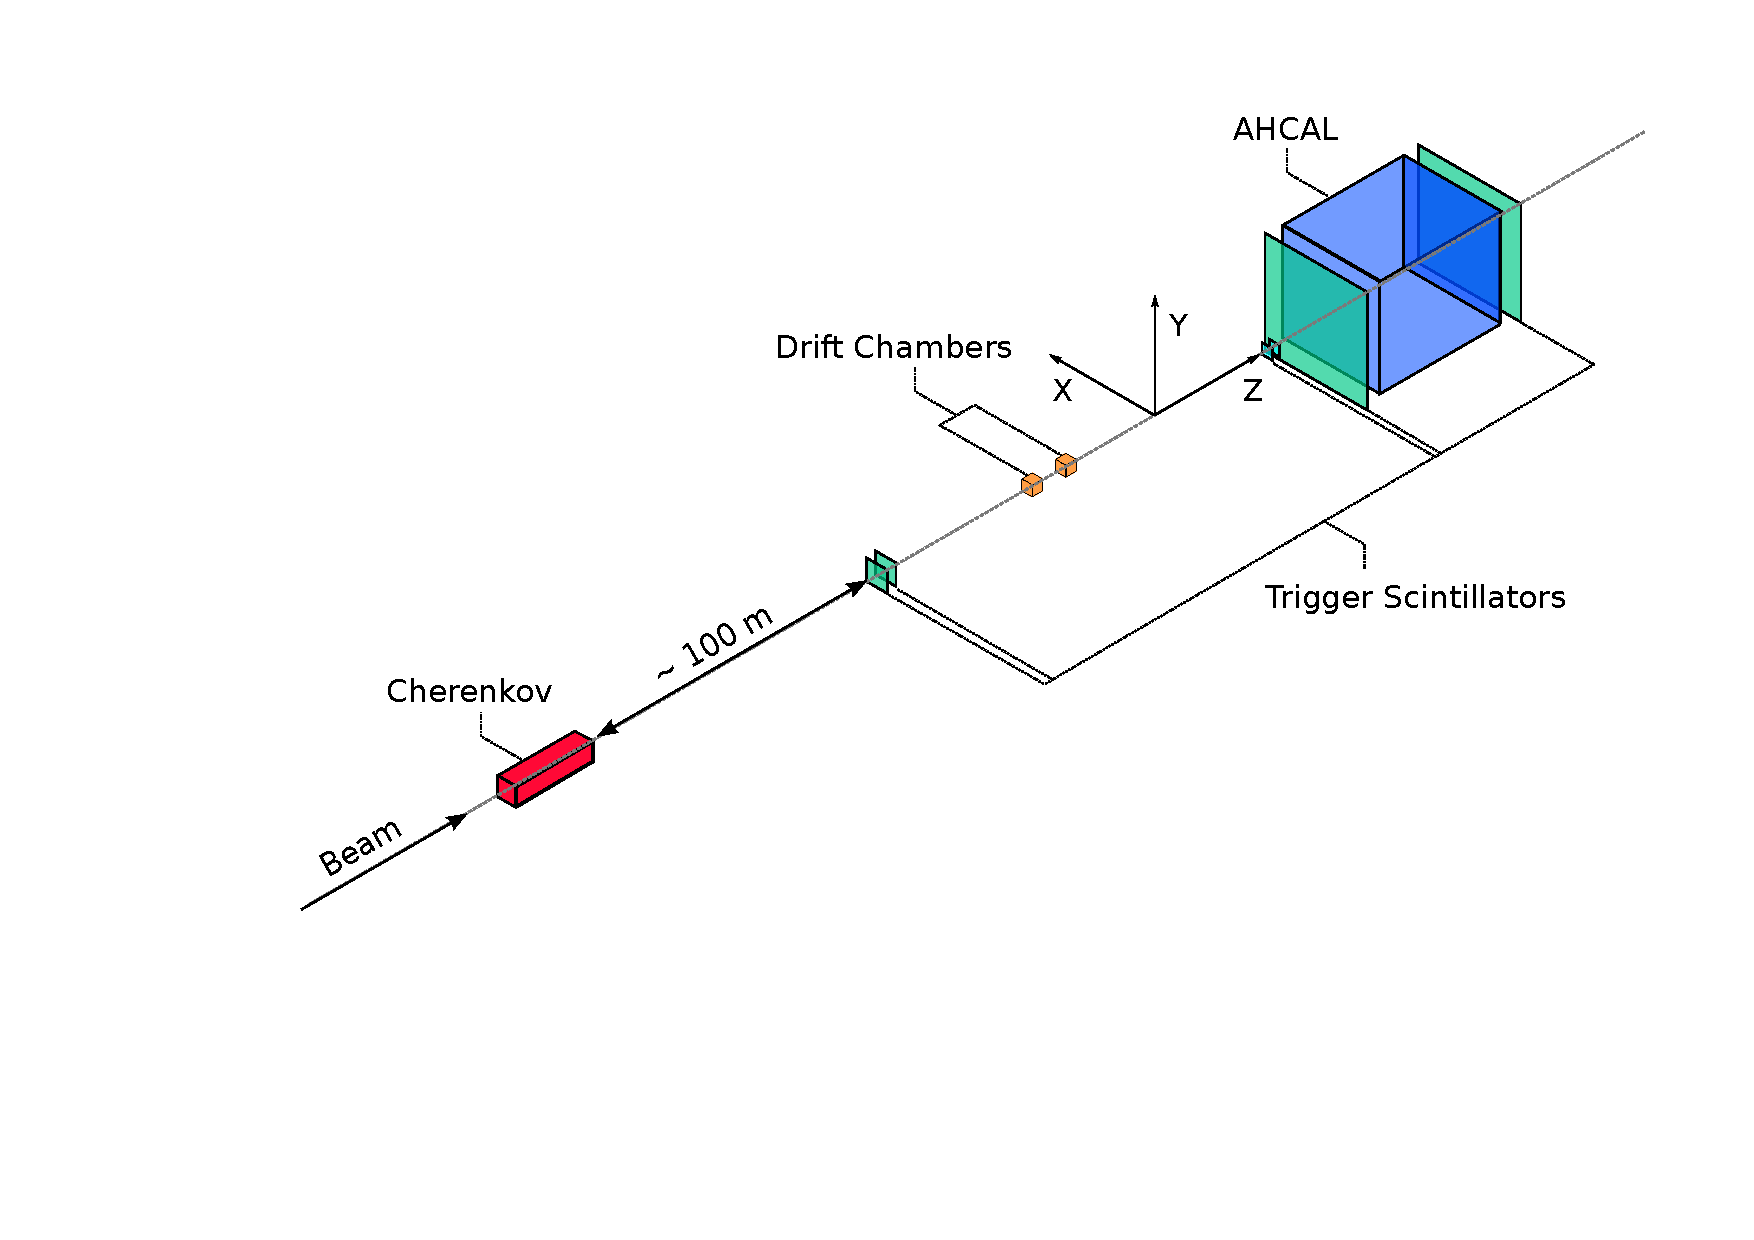
\includegraphics[width=0.7\linewidth]{fig/TestbeamSetup.pdf}
	\caption{Sketch view of the beamline setup at the CERN SPS H2 beamline in July 2015.} \label{fig:TestbeamScketch}
\end{figure}

The AHCAL is composed of 48 iron absorber plates in which 14 active layers are installed. The 10 first layers consist of single ECAL and HCAL Board Units (HBU) of a depth of around 10 X$_0$ ($\sim$ 1 $\lambda_{\pi}$) aiming to act as a shower start finder. The next four layers consist of 2 by 2 HBUs providing information about the development of pion showers at different depths. In total, the prototype has 3744 channels. It uses SiPM technology coupled to scintillator tiles of $3\times3$ cm$^2$ readout by an application specific integrated chip, the SPIROC2b \cite{5401891}. A diverse variety of SiPMs and tile designs were used in this testbeam, a detailed table of the SiPM characteristics can be seen in Table \ref{table:sipm_list}. The AHCAL detector is placed on a movable stage in order to be able to move the detector position relative to the beam for muon calibration runs.

\begin{table}[htb!]
	\centering
	\caption{Layer structure of the AHCAL in July 2015.}
	\label{table:muon_sel}
	\begin{tabular}{@{}lllll@{}}
		\toprule
		Absorber Slot \# & Layer \# & Abs. thickness before layer [X$_0$/$\lambda_{\pi}$] & Layer size [cm$^{2}$] & $N_{chn}$\\
		\midrule
    1-10 & 1-10 & $\sim$1/0.1 & $36\times36$ & 1440\\
    11 & 11 & $\sim$1/0.1 & $72\times72$ & 576\\
    13 & 12 & $\sim$2/0.2 & $72\times72$ & 576\\
    21 & 13 & $\sim$8/0.8 & $72\times72$ & 576\\
    31 & 14 & $\sim$10/1 & $72\times72$ & 576\\
		\bottomrule
	\end{tabular}
\end{table}

Scintillator plates in front and back of the calorimeter are used as a trigger signal that is provided to the AHCAL DAQ to validate events \cite{Kvasnicka:CR_IEEE2016}. Additionally, the coincidence signal from the scintillators is provided directly to several channels of the AHCAL in order to provide a reference time of the trigger as shown in table \ref{table:trigger_ref}. A Cherenkov detector, at around 100 m upstream, was available to tag incoming particles.

\section{Simulation}

The AHCAL simulation model is based on the \mokka \cite{MoradeFreitas:2002kj} framework v08-05-01 and the new \ddhep \cite{Frank:2014zya} framework v00-16, using the \geant v10.1 simulation. A right-handed coordinate system is used such that the Z-axis points in the beam direction and that the Y-axis is directed upwards. No beamline instrumentation is simulated except scintillator triggers in front of and behind the detector. A similar amount of material is achieved by filling the world volume with air and by adding 5.6 mm of lead ($\sim$ 1 X$_0$) directly at the calorimeter front face in order to account for missing upstream material. The beam gun is placed 1 m from the calorimeter front face and it is configured to generate single beam particles with a 2\% momentum spread according to the beamline beam parameters. Muons and electron showers are simulated using the QGSP\_BERT\_HP physics list. Pion showers are simulated using QGSP\_BERT, QGSP\_BERT\_HP and QBBC physics lists.

\subsection{Geometry and Digitization}
\label{sec:GeoDigi}

The AHCAL simulation model consists of 32 absorber layers and 14 active layers. Each absorber layer are made of stainless steel 17.2 mm thick. Each active layer is primarily composed of 1 mm steel cassette, 0.7 mm PCB, 2 or 3 mm scintillator strip or tile. The density and composition of the scintillator is taken as default provided in \geant.

The digitization of simulated hits is very similar to the previous AHCAL physics prototype \cite{1748-0221-5-05-P05004}. Individual calibration factors obtained from data are used to extract the light yield which is needed to model the statistical fluctuations of photons hitting a SiPM \cite{Hartbrich:2016bbz}. Saturation effects are also included using a global parameter, the number of pixels available on each SiPM type, as no measurement of the saturation curve is available. Most of the tiles used are wrapped with a reflective foil such that crosstalk effects between channels can be neglected. For layers with no wrapping, a default value of 15\% cross-talk is used. Noise is extracted from muon runs and overlaid onto simulated events. Dead channels and channels without calibration factors (MIP, gain, pedestal) are rejected.

The timing of simulated hits is modeled as in the SPIROC2b, the energy from sub-hits in a cell is integrated over a sliding time window of 15 ns, if the energy sum of the sub-hits in this time window passes the energy threshold, the time of the sub-hit passing the energy threshold is used as the time of the simulated hit. To simulate detector resolution effects, the time of a simulated hit is smeared with a double Gaussian function, with parameters determined from data, and is convoluted with a Gaussian function with a sigma depending on the number of triggered channels in a chip parametrized from data (see section \ref{sec:NumberTrigger}).

After the digitization, all simulated hits have the same format as raw data hits and are reconstructed with the same software chain that is used for data. To suppress noise hits, only hits above 0.5 MIP are considered in this study.

\subsection{AHCAL Model Validation}

Prior to the time analysis, the simulation and digitization are validated. Comparisons of electromagnetic interactions in the AHCAL are done as such interactions should be well described in simulation. Firstly, the simulation must be validated at the lowest hit energies. The comparison of the spectrum of a MIP-like particle traversing the AHCAL was done and is shown in figure \ref{fig:MIPData_MC}. The shape of the spectrum matches relatively well. The data appears slightly wider than for simulation because of channel-by-channel mis-calibrations that are not modeled in the simulation. The figure \ref{fig:ProfileMIP_Edep} shows the longitudinal mean energy profile for muon-like tracks in data and simulation. The data is reproduced by the simulations within 3-4\%.

\begin{figure}[htbp!]
	\centering
	\begin{subfigure}[t]{0.49\textwidth}
		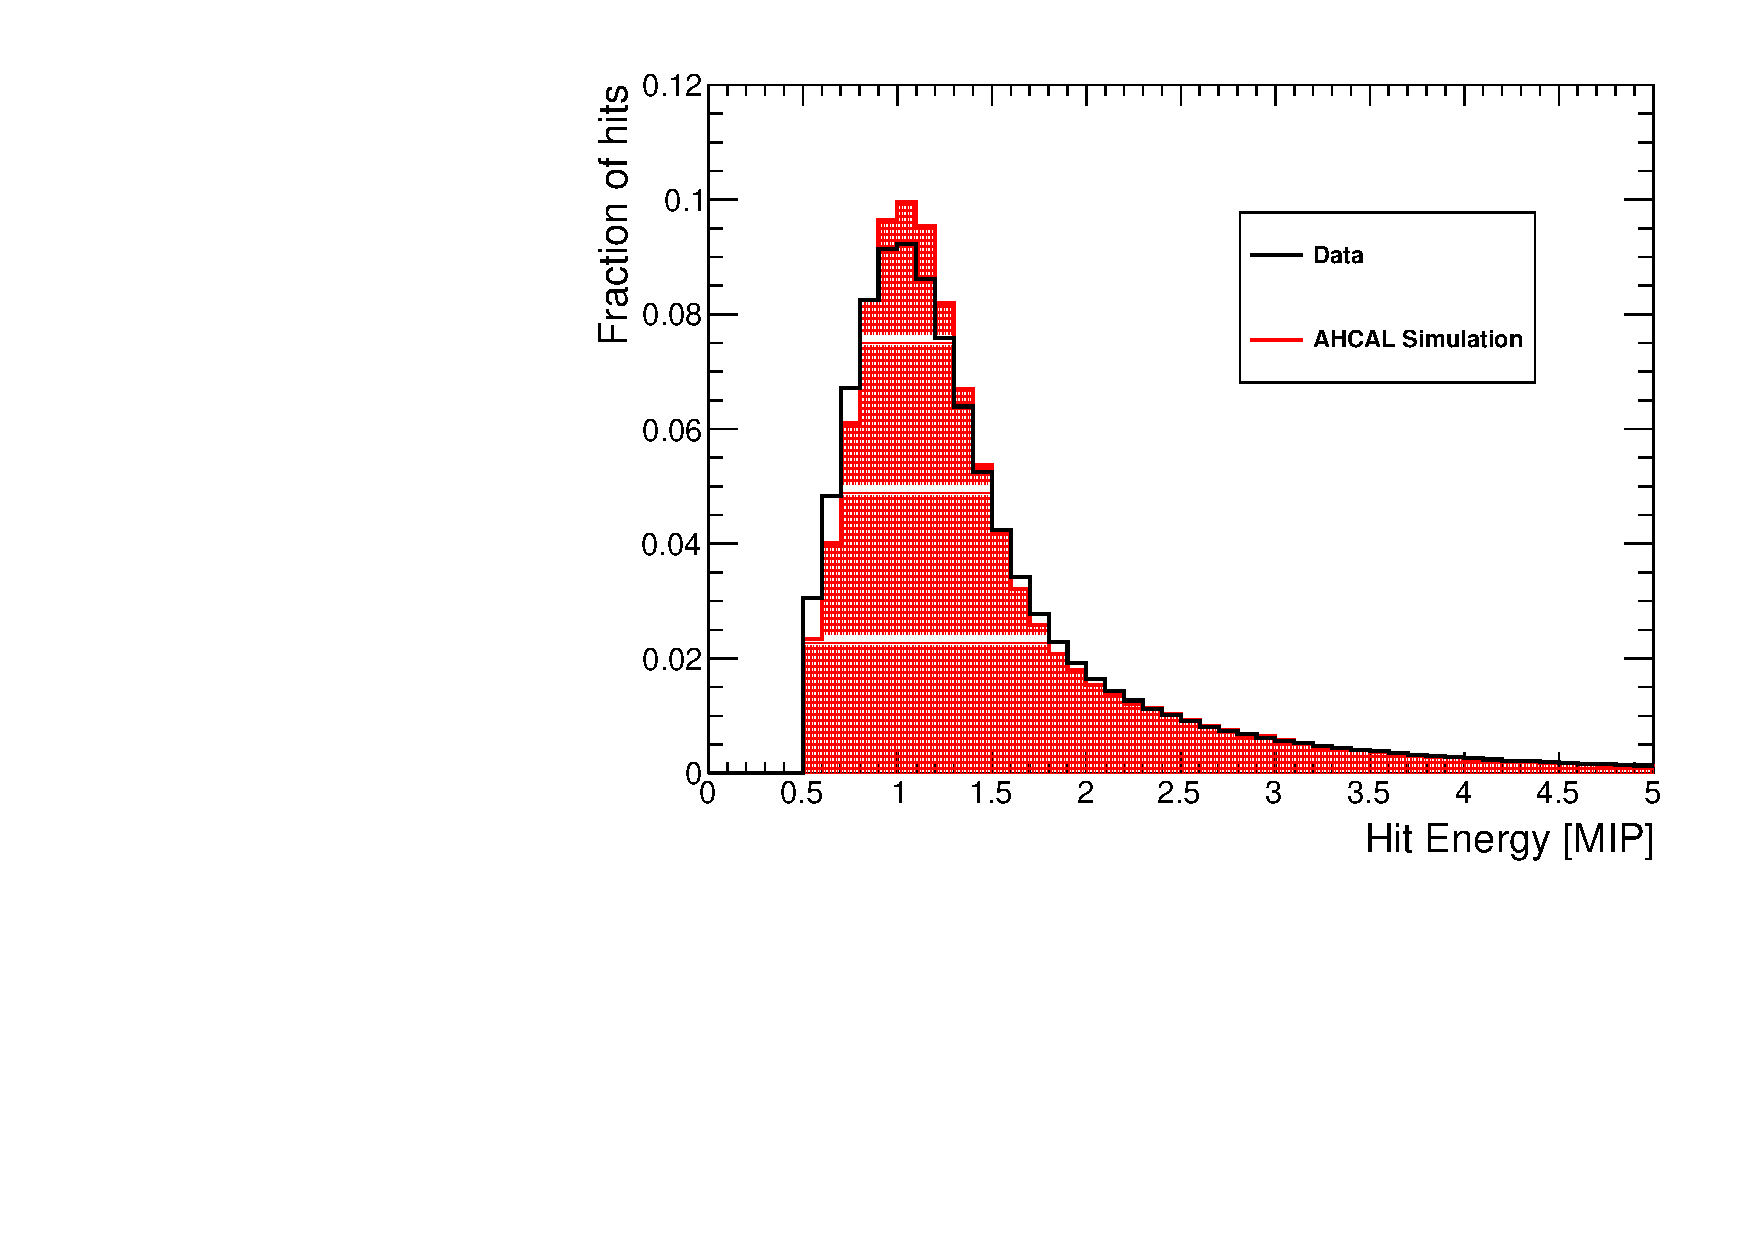
\includegraphics[width=1\linewidth]{fig/ComparisonMCData_MIPPeak.pdf}
		\caption{} \label{fig:MIPData_MC}
	\end{subfigure}
	\hfill
	\begin{subfigure}[t]{0.49\textwidth}
		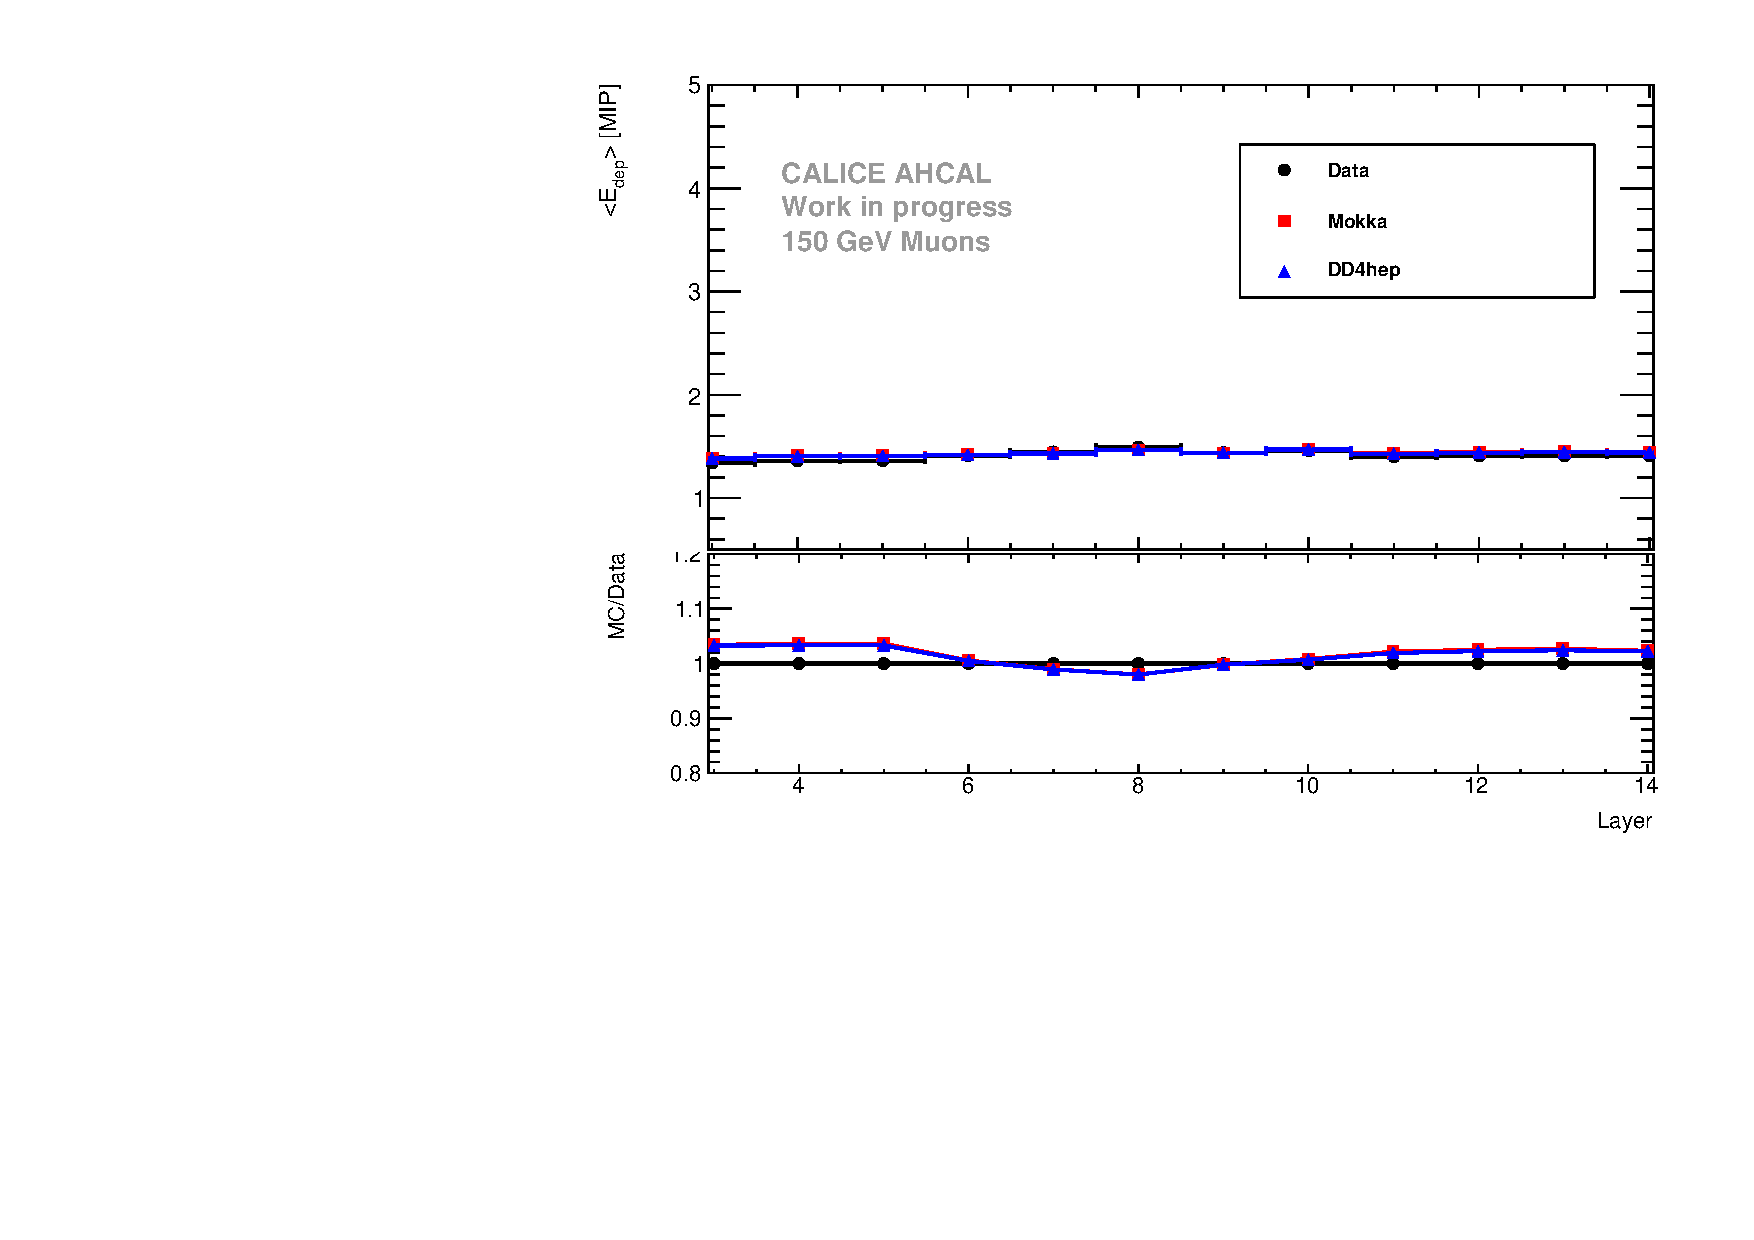
\includegraphics[width=1\linewidth]{fig/ProfileMuons_Edep.pdf}
		\caption{} \label{fig:ProfileMIP_Edep}
	\end{subfigure}
	\caption{\subref{fig:MIPData_MC}) Hit Energy Spectra for the complete AHCAL for muon like-track hits for both data and simulation. \subref{fig:ProfileMIP_Edep}) Longitudinal mean energy profile for muon like-track hits in data and simulations..}
	\label{fig:Val}
\end{figure}

Further comparison were made using the electron dataset. The figure \ref{fig:HitEnergy10GeVe} shows the hit energy spectra for 10 GeV electron showers in data and simulation. Hit energies up to 60 MIPs are well described by the simulation up to 10\%. A small difference is noticeable around 20 MIPs because of overestimated intercalibration factors between high gain hits and low gain hits that shift the hit energy to slightly higher values. The simulation is underestimating the hit energy by a large factor over 60 MIPs. It is similar at higher beam energies. The underestimation in simulation of the hit energy comes from an incorrect value of the number of effective pixels used in the saturation function to saturate hits in the simulation. This number is too small thus saturating the simulation to lower hit energies. However, for this analysis, only energies below tens of MIPs is relevant (see section \ref{sec:TWCorr}) and well described by the simulation.

\begin{figure}[htbp!]
	\centering
	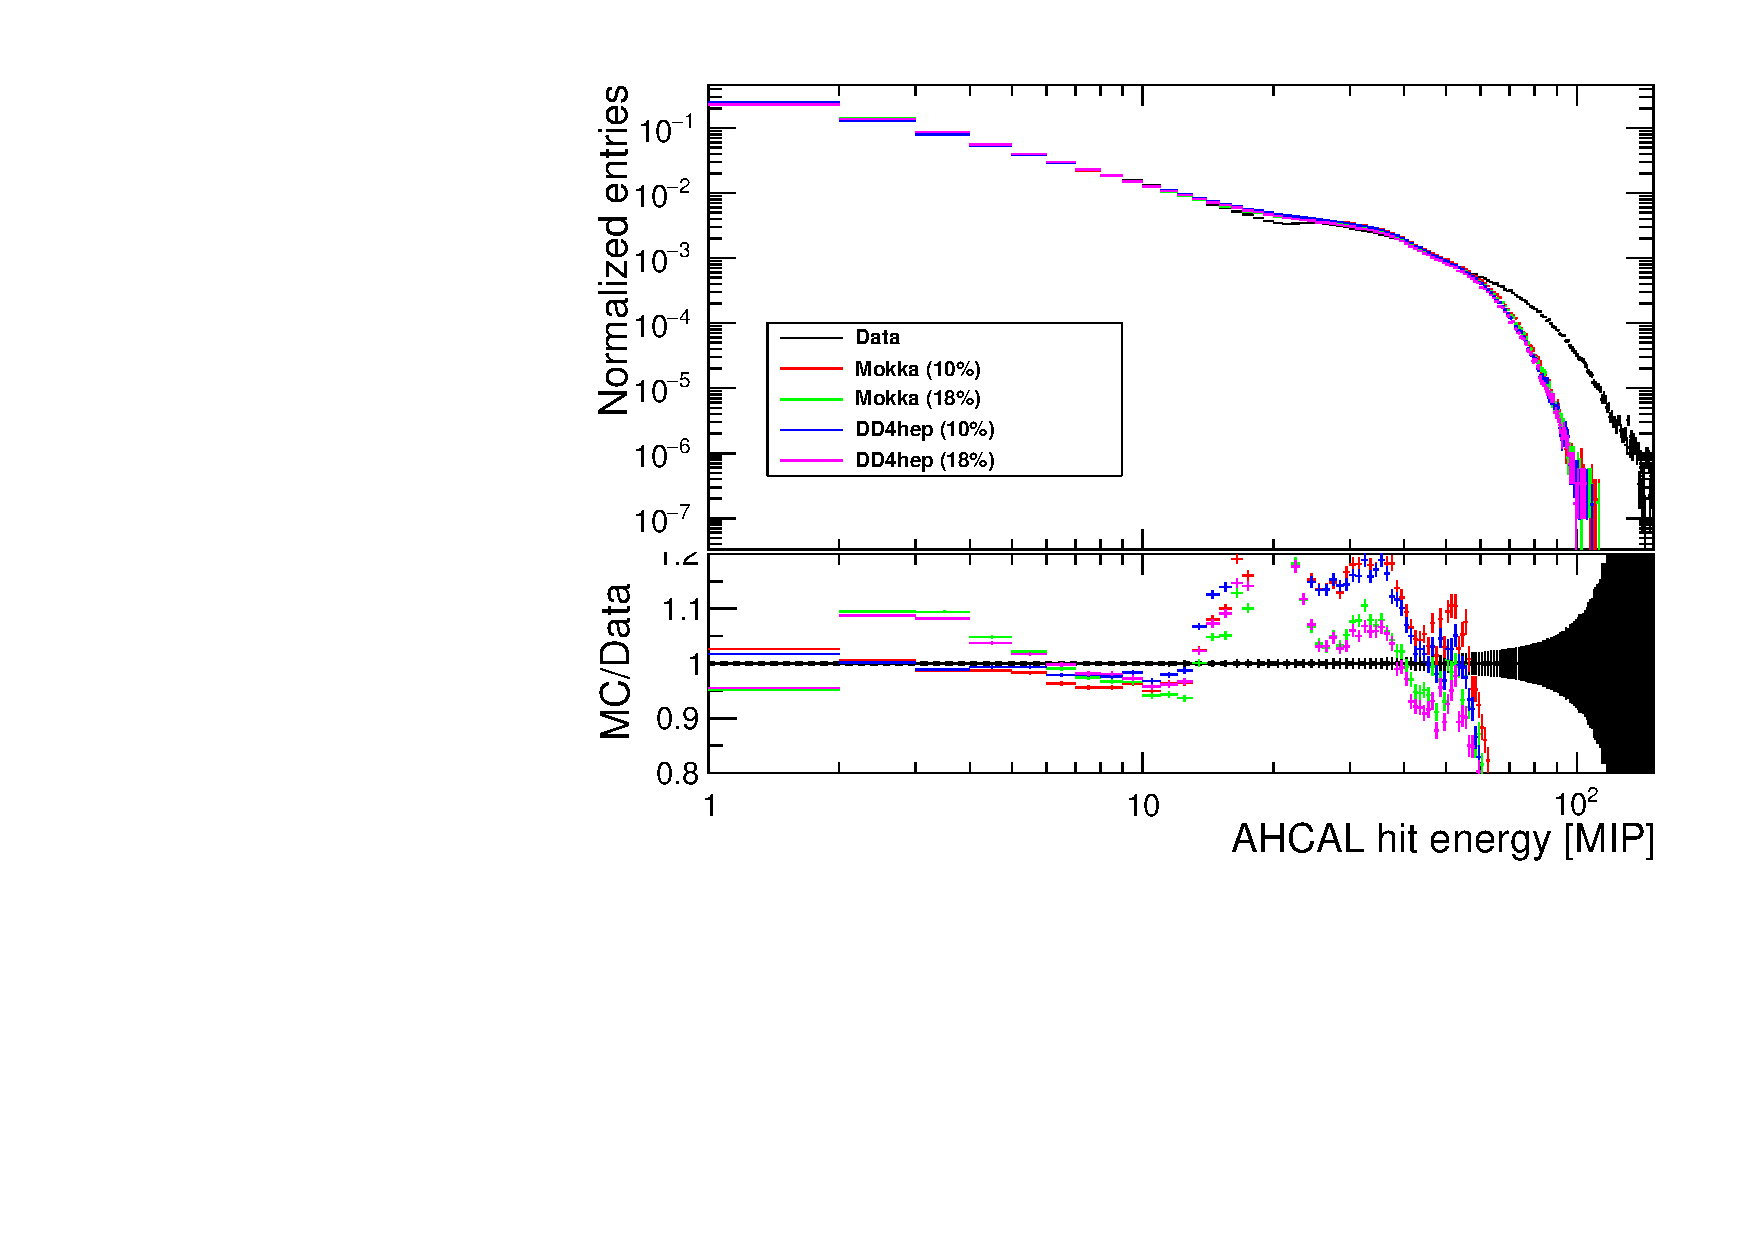
\includegraphics[width=0.7\linewidth]{fig/HitEnergy_Electrons10GeV.pdf}
	\caption{Electron hit energy spectra for data and simulation for 10 GeV beam energy. The different colors corresponds to the variation of the cross-talk parameter in the simulations between 10\% and 18\%.} \label{fig:HitEnergy10GeVe}
\end{figure}

% \begin{figure}[htbp!]
% 	\centering
% 	\begin{subfigure}[t]{0.49\textwidth}
% 		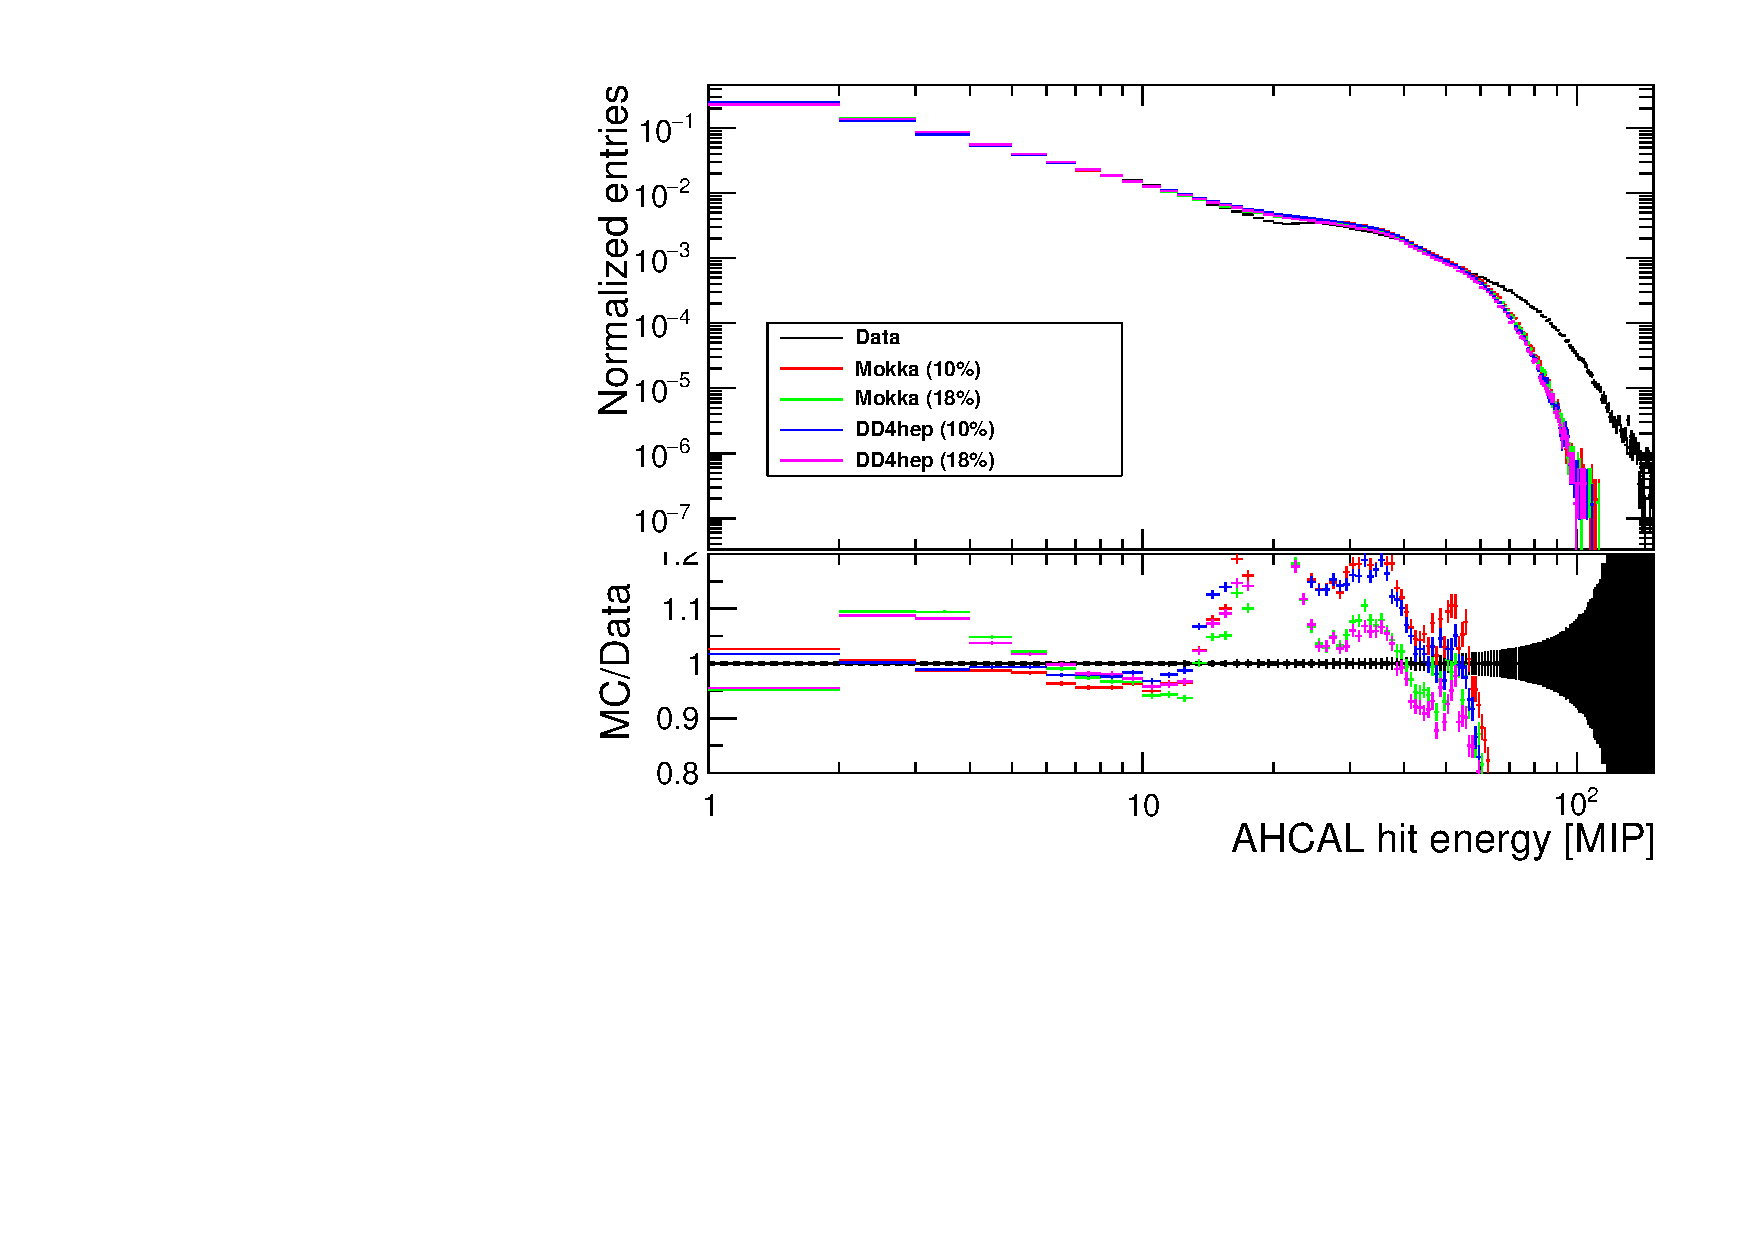
\includegraphics[width=1.\linewidth]{fig/HitEnergy_Electrons10GeV.pdf}
% 		\caption{} \label{fig:HitEnergy10GeVe}
% 	\end{subfigure}
% 	\hfill
% 	\begin{subfigure}[t]{0.49\textwidth}
% 		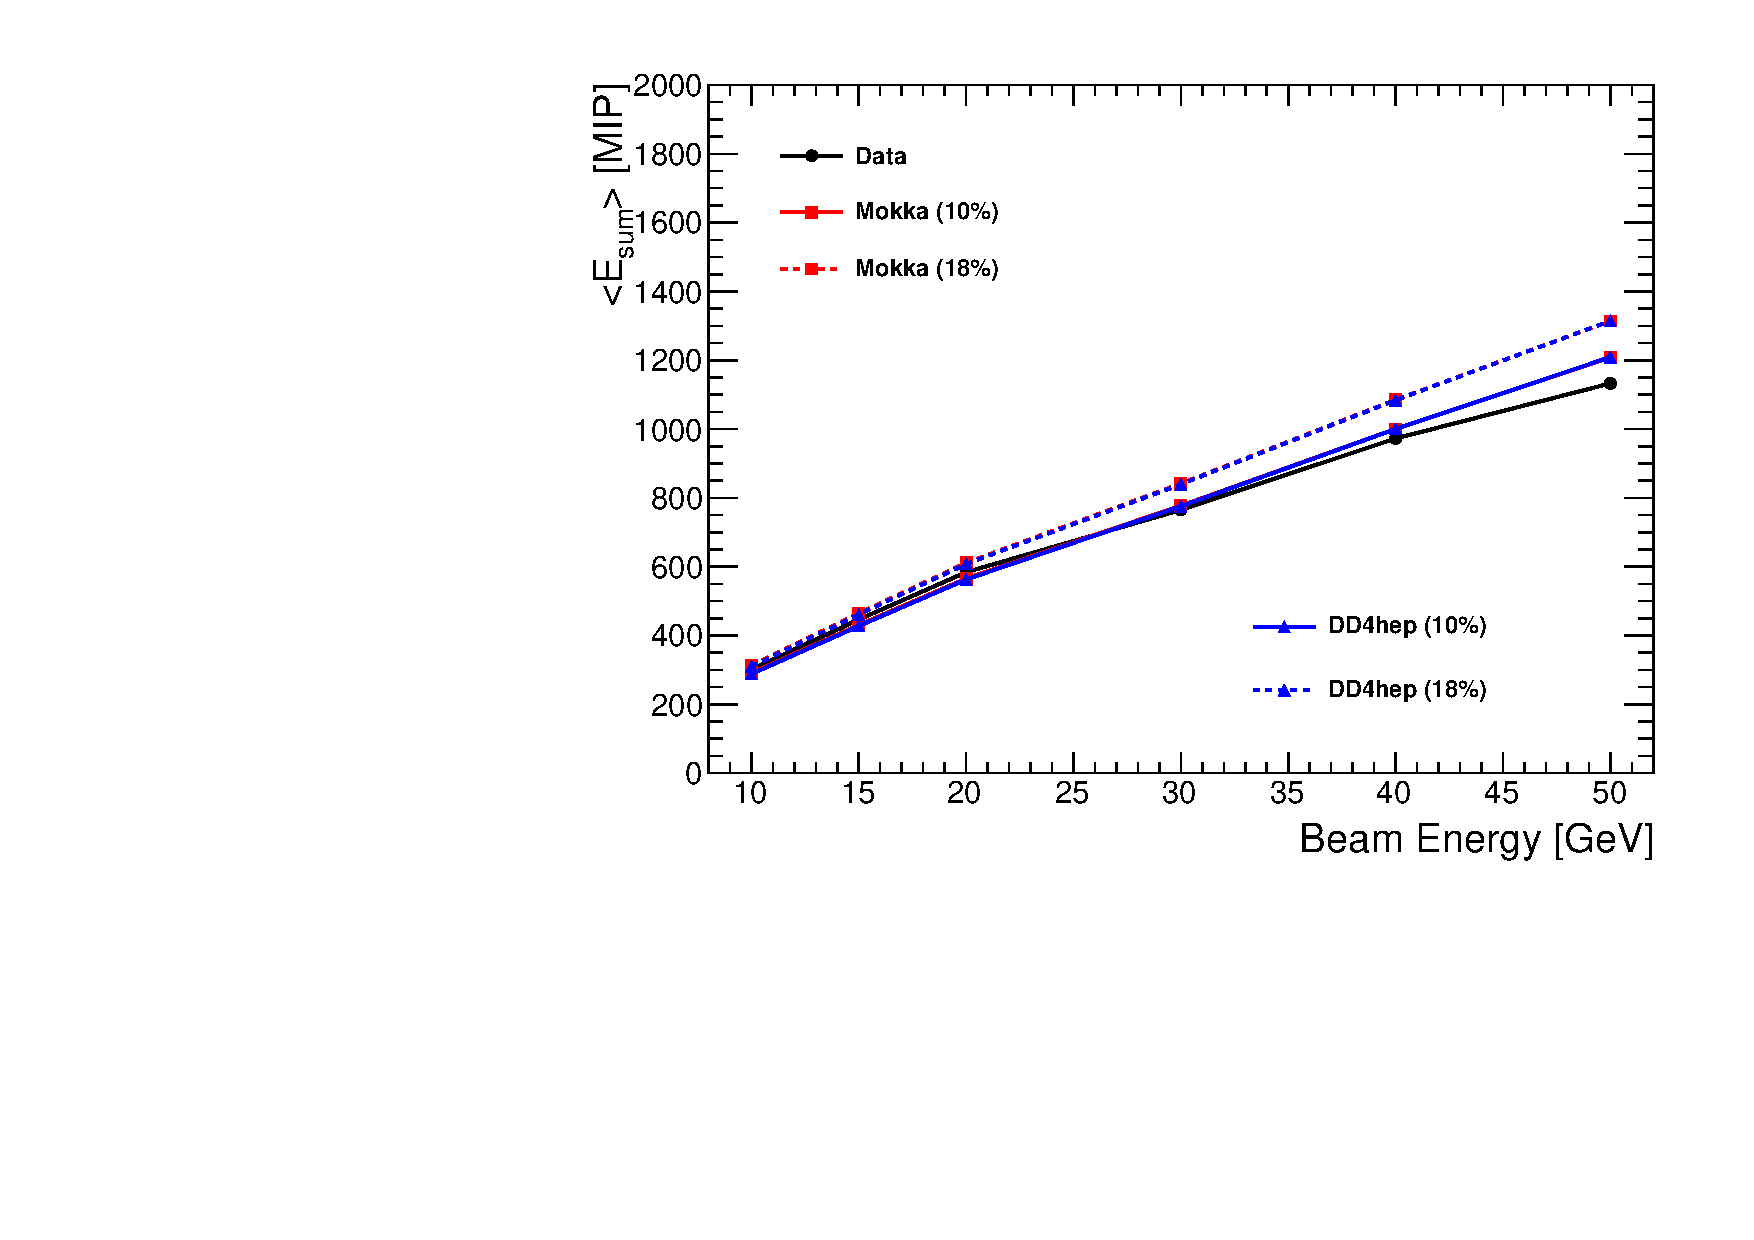
\includegraphics[width=1.\linewidth]{fig/EsumElectrons_BeamEnergy.pdf}
% 		\caption{} \label{fig:EsumMeanElectron}
% 	\end{subfigure}
% 	\caption{\subref{fig:HitEnergy10GeVe}) Electron hit energy spectra for data and simulation for 10 GeV beam energy. The different colors corresponds to the variation of the cross-talk parameter in the simulations between 10\% and 18\%. \subref{fig:EsumMeanElectron}) Comparison of the mean energy sum in the AHCAL as function of the beam energy for electron data and simulations with different cross-talk parameters. Simulated with QGSP\_BERT\_HP in \geant v10.1.}
% 	\label{fig:eHitVal}
% \end{figure}

A more detailed energy analysis of the CERN 2015 July data in the AHCAL is in preparation \cite{AmbraPrivate}. The simulation does not describe perfectly the data especially for higher electron beam energies, but reflects the data around 10-20\%. However, the description of electromagnetic showers in simulations is deemed satisfactory for the study of the time development of hadron showers.

\section{Event Selection}

\subsection{Muon selection}

To select muons, an event pre-selection and a track finder \cite{Hartbrich:2016bbz} selection is performed. A cut on the number of hits in the AHCAL is done at 20 as the number of hits should be around 1 per layer for a MIP-like particle plus the number of noise hits expected in the detector. The track finder algorithm selects AHCAL towers of hits in the same $x:y$ position and it rejects AHCAL towers that contains less than a certain number of hits. In order to select muons or punch-through pions, a straight track of at least 7 hits is required in the whole AHCAL. This assumes that the calorimeter was perfectly perpendicular to the beam, therefore any tilted tracks would be missed. In addition, to reject late pion showers, no more than 2 hits are allowed per layer to account for some flexibility with noise hits. A summary of the muon selection is shown in table \ref{table:muon_sel}. The selection efficiency is 72.5\% for muons, <0.1\% for electrons and 5\% for pions which is compatible with the fraction of pion traversing the AHCAL without hard interaction.

\subsection{Electron selection}

Electron events are needed to validate the timing behavior in simulation as well as the detector simulation model. It is important to have a clean sample of electrons to cross-check the timing calibration. An electron selection is done using the beam instrumentation and layer information. Events with a Cherenkov tag are used. The energy deposit in the first three AHCAL layers ($E_3+E_4+E_5$) must be over 10 MIPs. A box cut on the number of hits and the center of gravity in the z direction is done. As the number of hits in a electron shower is proportional to the shower energy, this cut is energy dependent. The energy deposited in the last two layers relative to the energy deposited in the calorimeter ($(E_{13}+E_{14})/\Sigma E$) is required to be under 1\% to reject pion showers and to contain the electron shower. The electron selection is summed up in table \ref{table:electron_sel}. The selection efficiency is <0.1\% for muons, between 96-91\% for electrons between 10 and 50 GeV and 15.9-1.1\% for pions between 10 and 50 GeV. A significant fraction of pion remains at low energies, however, there is confidence that no pion contamination is present due to the pure electron beam generation with the beamline.

\subsection{Pion selection}
\label{sec:pionsel}

The goal of the pion selection is to reject punch-through pions, muons and possible electron contamination as these events would be instantaneous. The events without a Cherenkov tag are selected. The number of hits required per event needs to be over 20 to reject most muons or punch-through pions without cutting on the center of gravity in z in order not to bias the start of the pion shower. The energy fraction deposited in the two last AHCAL layers must be over 1\% in order to ensure that pion showered and reject possible electron showers. The number of hits in the two first AHCAL layers $N_3+N_4$ must be under 5 to mitigate possible particle contamination from electrons. In addition, multiple particle events were observed in the data. As no beam instrumentation could be used for rejecting these events, a rejection method based on the hit time information was developed. The method is the following: all the hits in an event are placed and ordered in time; Then for each hit after 50 ns, a timing window of 30 ns is looked after. The number of hits in that window is counted. If the number of hits is over 5, it is classified as a \textit{late cluster}. The event is rejected if there is at least one late cluster. The multi-particle event rejection has been checked on simulated data and affects the selection between <0.1\% up to 2\% from 10 to 90 GeV pions. These multi-particle events are also suppressed in data. The number of events removed varies between 0.1\% and 1\% depending on the beam energy. However, due to the calorimeter not being fully equipped thus providing limited information, some contamination by multi-particle may remain in the data. The table \ref{table:pion_sel} shows the selection cuts for the pion data. The selection efficiency is 0.1-1\% for muons, <0.1\% for electrons and between 29.9 and 51\% for pions between 10 and 90 GeV.

\section{Timing calibration of the AHCAL}

In a first time, the muon data is used to determine the parameters for the timing calibration. Muons are used because the process they induce is quasi-instantaneous. In a second step, the calibration is cross-checked using the electron data as also EM showers are quasi-instantaneous. This enables a verification of the time calibration procedure and may reveal effects that are not present in the muon data.

\subsection{Time recording in the SPIROC2b}

The SPIROC2b ASIC can readout 36 SiPM-channels capable to measure the charge with two gains (high and low gain) and time for each channel. Each channel is equipped an analog memory, called memory-cells, with a depth of 16 events to store the energy and time measurement. Additionally, the ASIC can be operated in external or auto-trigger mode with a configurable threshold. The ASIC has two multiplexed TDC voltage ramp to avoid deadtime between each clock cycle that are common to all channels. The time information provided by the SPIROC2b in the data is in TDC units. Similar to the ADC scale, it would be difficult to compare directly channels using the TDC unit. The TDC information needs to be interpreted into a common unit of time, the nanosecond. The TDC information of each channel can be converted into nanoseconds following the simple schematic shown in figure \ref{fig:ConvertTime}.

\begin{figure}[htbp!]
	\centering
	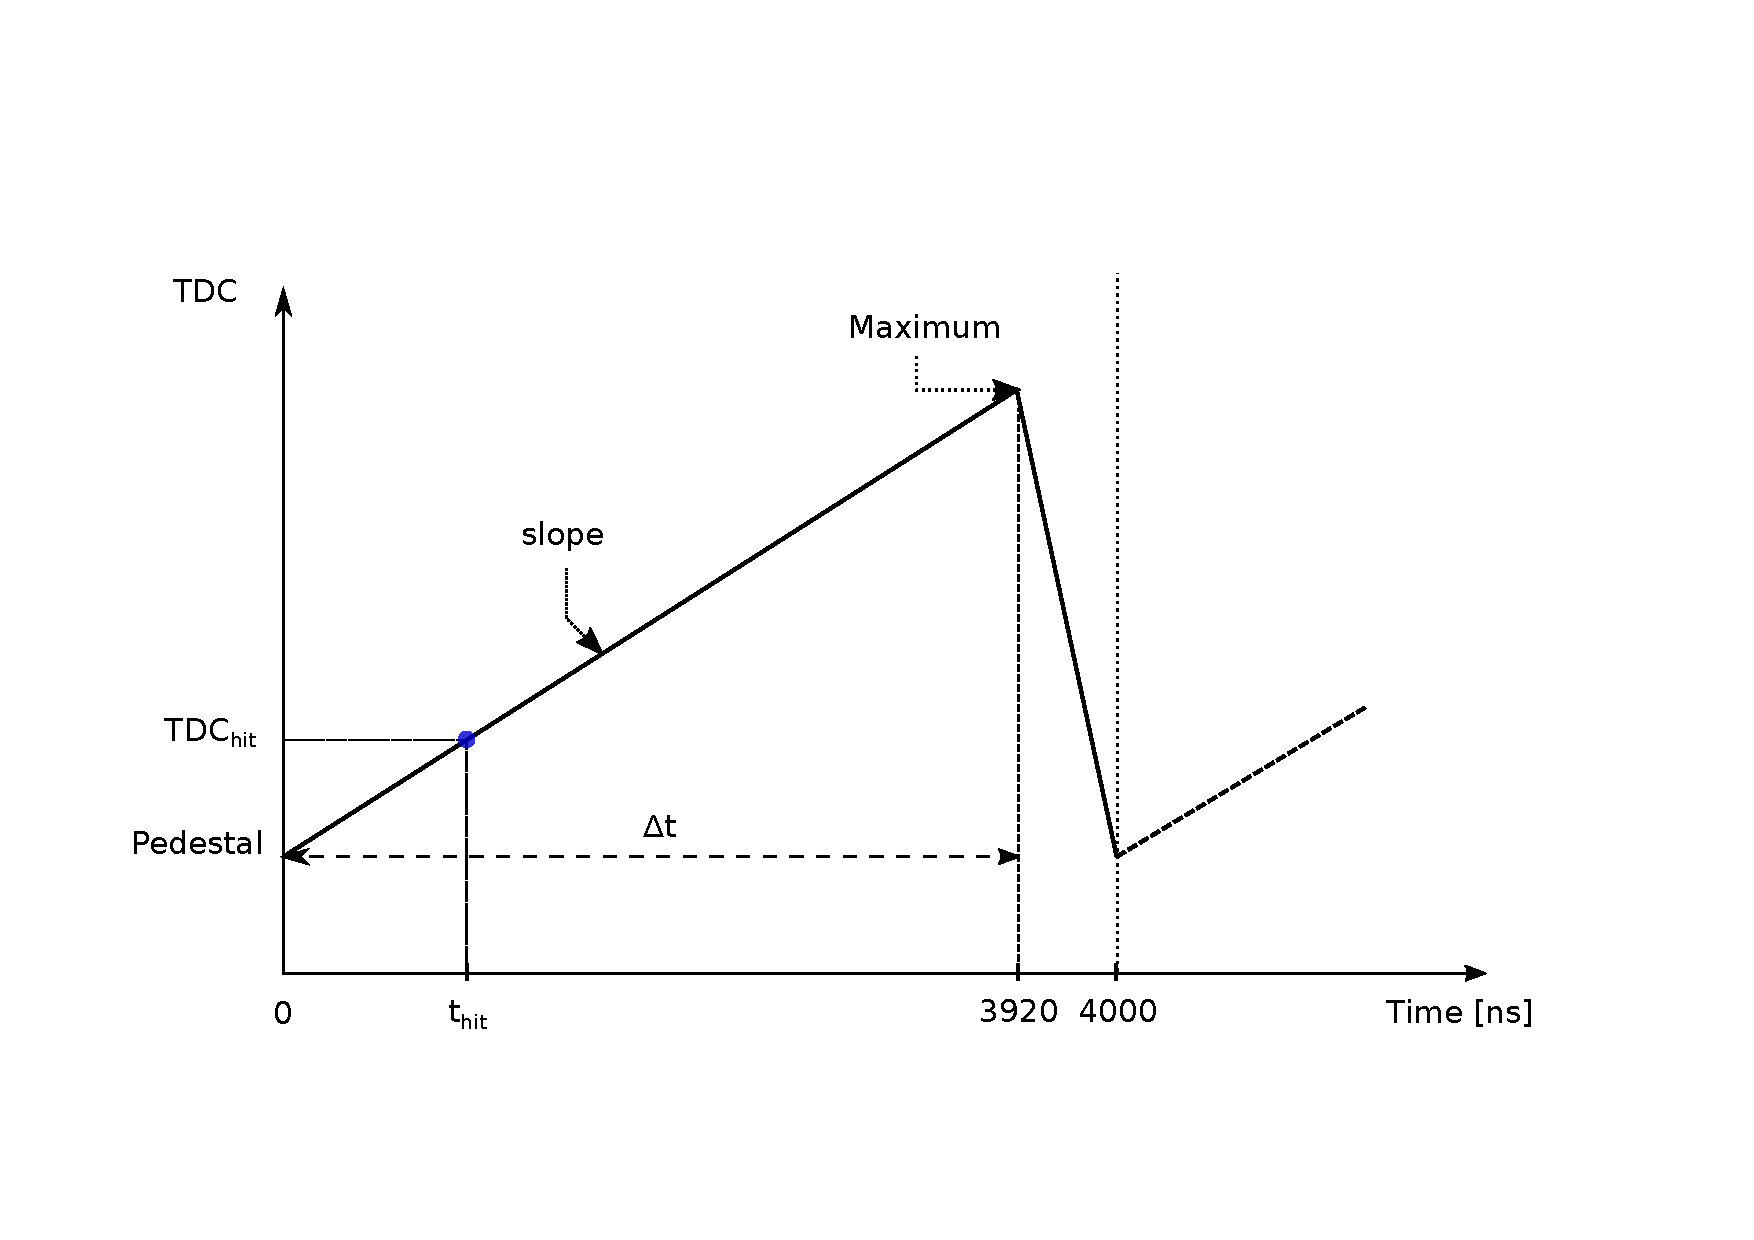
\includegraphics[width=0.9\linewidth]{fig/TDCRamp.pdf}
	\caption{Schematic of the TDC ramp in the SPIROC2b used in testbeam with a slow clock of 250 kHz. The slope of the ramp is $\Delta_t$/(Max-Ped). The time of the hit is then calculated as the following: t$_{Hit}$ = slope $\times$ (TDC$_{Hit}$ - Ped).} \label{fig:ConvertTime}
\end{figure}

In order to determine the ramp slope, the starting point or pedestal of the ramp and the endpoint of the ramp are measured. Since the SPIROC2b has two TDC ramps, each defined by a BXID parity (even or odd), two slopes need to be extracted per chip. While the memory-cells are different leading to offsets in pedestals thus 16 calibration values are needed per channel. The extraction of the slope and the determination of the pedestal is described in the following sections.

\subsection{Timing calibration procedure}

The timing calibration procedure of the AHCAL is quite tedious and requires a lot of steps. An overview of the steps performed for the time calibration of each individual AHCAL channels is shown in figure \ref{fig:CalibOverview}.

\begin{figure}[htbp!]
	\centering
	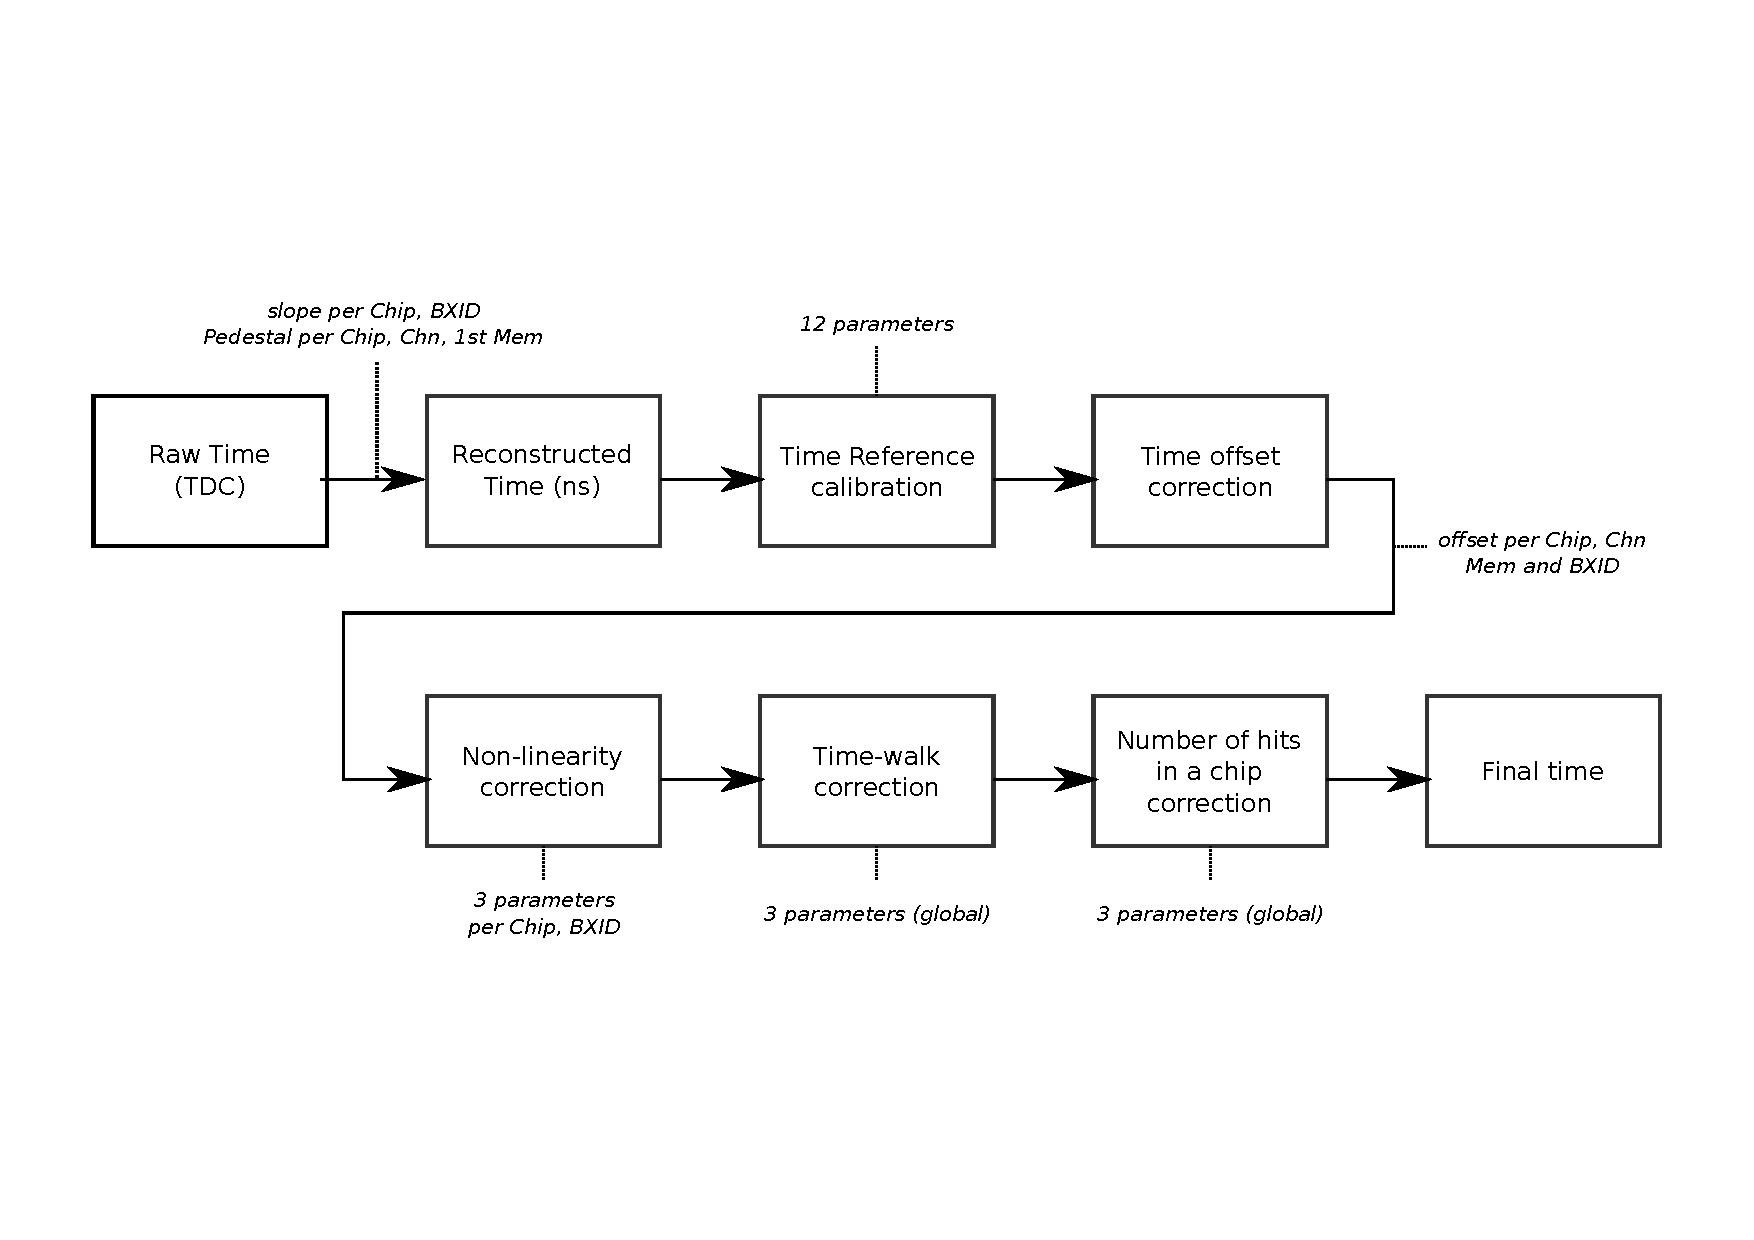
\includegraphics[width=1\linewidth]{fig/TimeCalibOverview.pdf}
	\caption{Overall view of the different steps performed for the AHCAL timing calibration. In total, more than 20000 constants are needed.} \label{fig:CalibOverview}
\end{figure}

\subsection{Slope and Pedestal extraction}

To reconstruct the time in a channel, the TDC value measured needs to be converted into nanoseconds. The slope is calculated as
\begin{equation} \label{eq:slope}
	s \: \text{[ns/TDC]} = \frac{3920}{b - a}
\end{equation}
where $s$ is the TDC ramp slope, $b$ is the endpoint of the TDC ramp and $a$ is the start point of the TDC ramp that is referred in the following as the pedestal. The total length of the ramp is 3920 ns instead of the expected value of 4000 ns due to a deadtime of around 2\% \cite{Brianne2012} induced by the multiplexer that switches between the two TDC ramps.

\begin{figure}[htbp!]
	\begin{subfigure}[t]{0.49\textwidth}
		\centering
		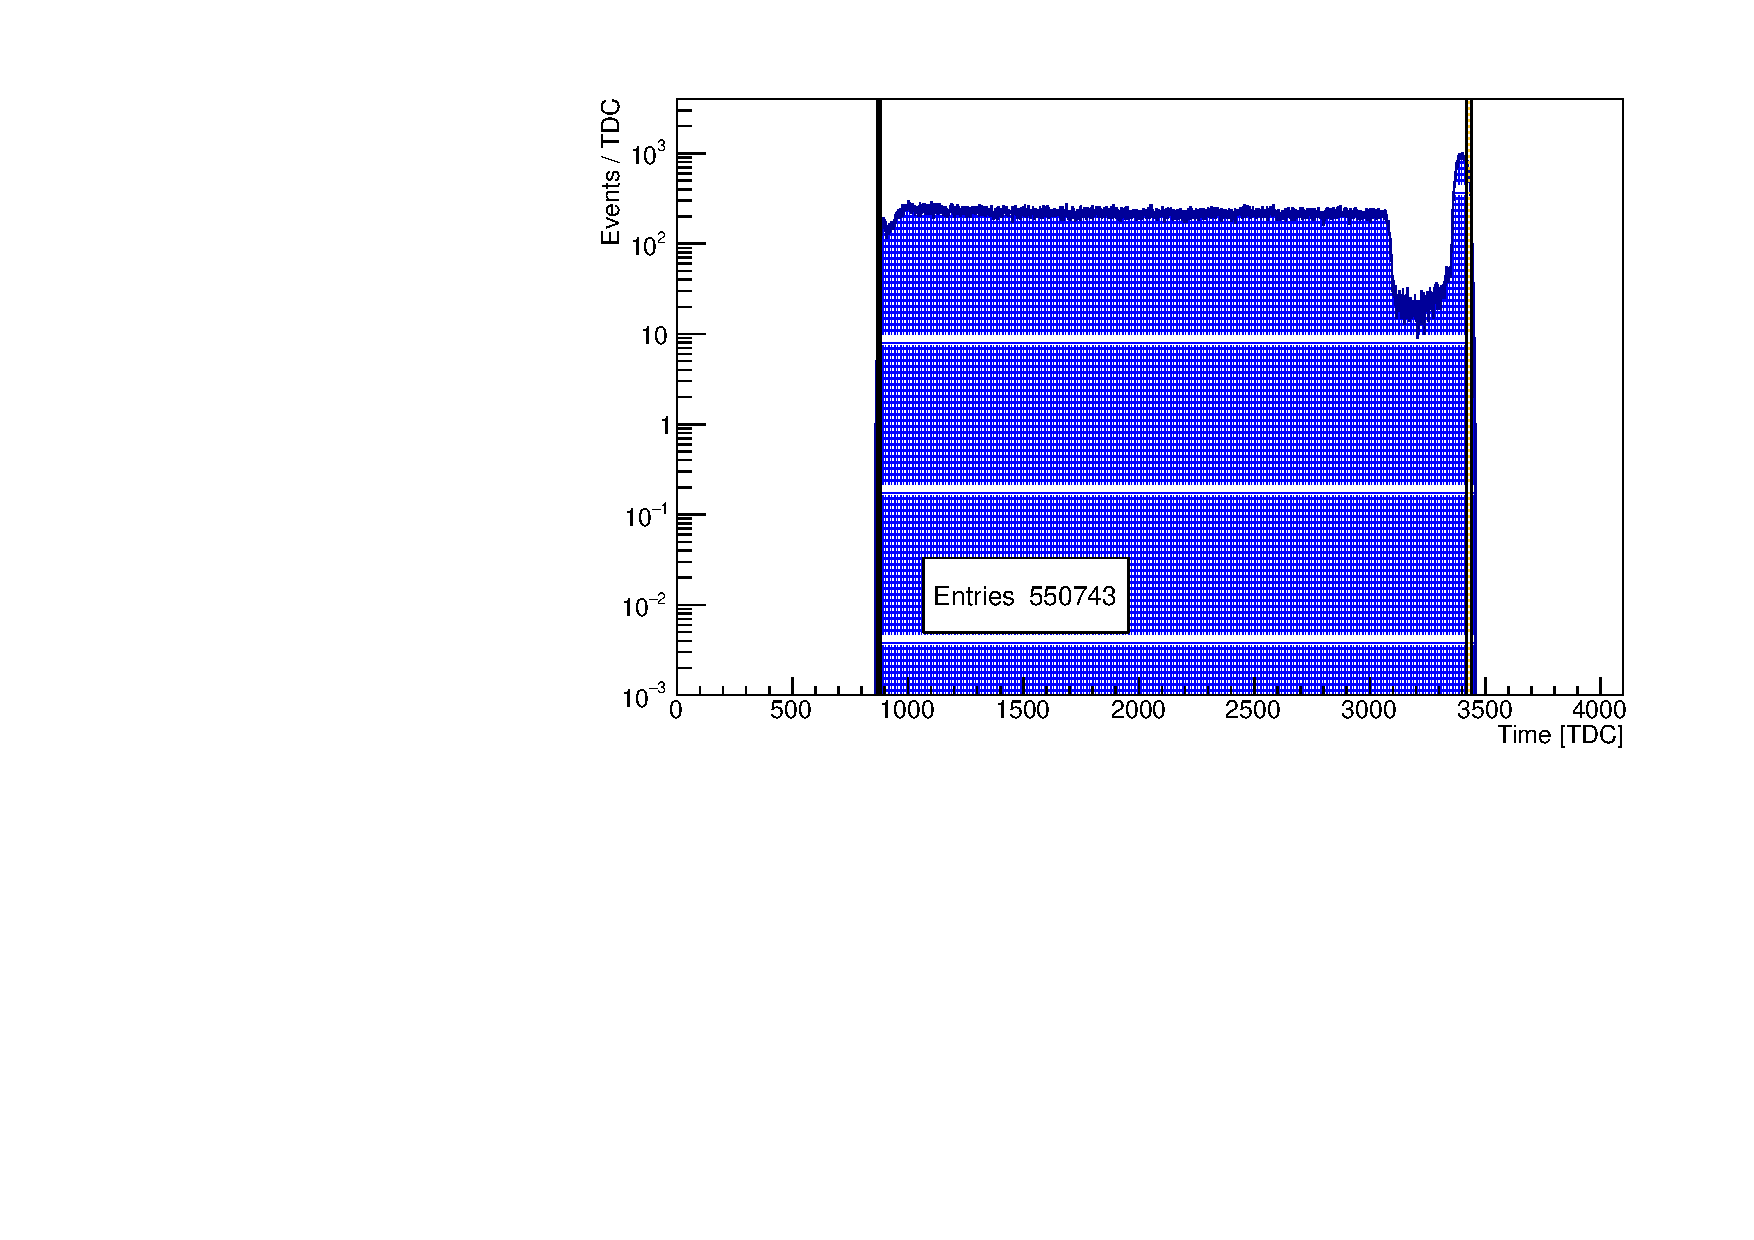
\includegraphics[width=1\linewidth]{fig/ExampleTDCSpectra.pdf}
		\caption{} \label{fig:TDC_Spectrum}
	\end{subfigure}
	\hfill
	\begin{subfigure}[t]{0.49\textwidth}
		\centering
		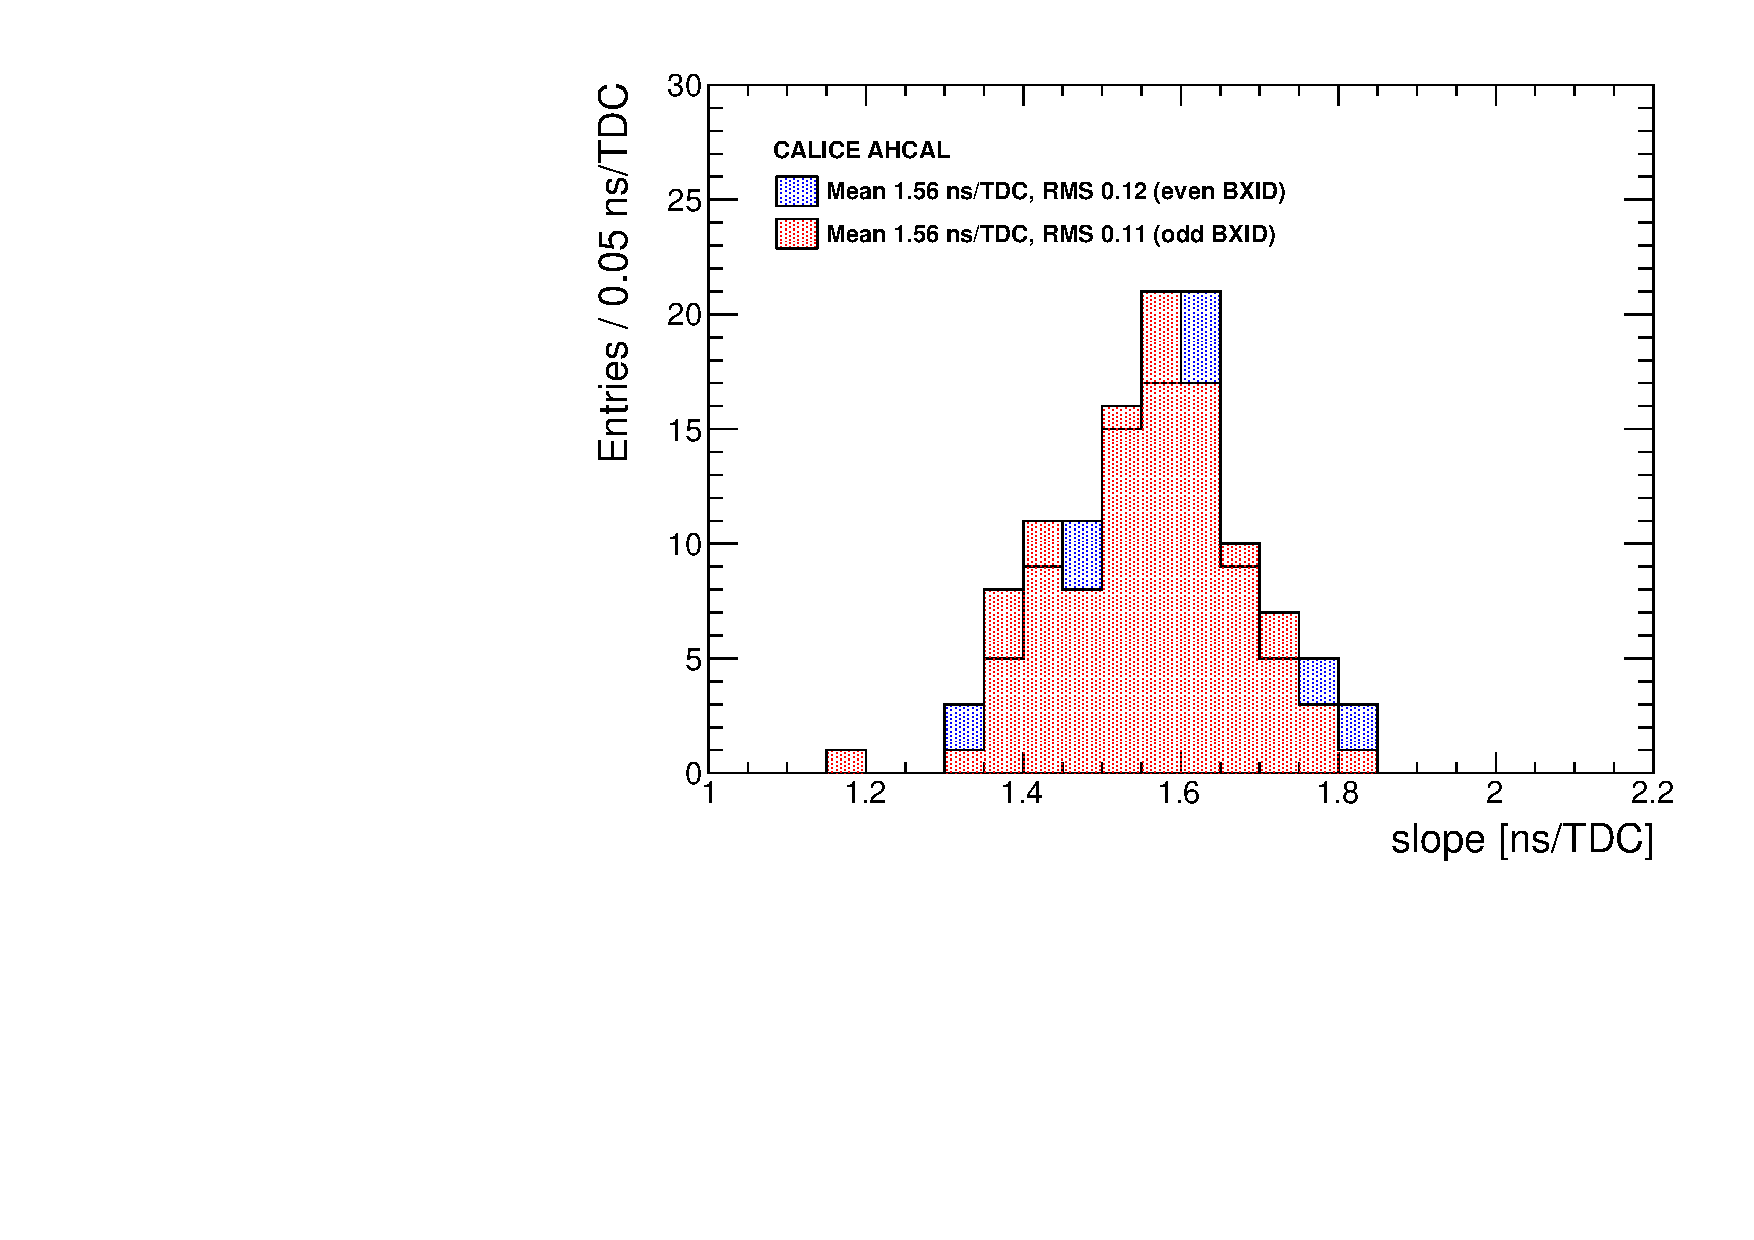
\includegraphics[width=1\linewidth]{fig/SlopesTDC.pdf}
		\caption{} \label{fig:slopes}
	\end{subfigure}
	\caption{\subref{fig:TDC_Spectrum}) TDC spectrum of a typical chip. The black lines indicate the fitted Max and Pedestal parameters for this chip. The yellow bands represent the uncertainty on the extraction of the parameter $a$ and $b$. The extracted parameters are $s$ = 1.47 $\pm$ 0.01 ns/TDC, $a$ = 888 $\pm$ 5 TDC and $b$ = 3613 $\pm$ 8 TDC. \subref{fig:slopes}) Distribution of the fitted slopes for even and odd bunch-crossing IDs. $\mu_{odd}$ = 1.564 ns/TDC, RMS$_{odd}$ = 0.121, $\mu_{even}$ = 1.556 ns/TDC, RMS$_{even}$ = 0.113. In total, 208 TDC slopes were extracted.}
\end{figure}

At a first order, the slope of the TDC ramp is assumed to be linear. The parameters $a$ and $b$ are extracted from the TDC spectrum of a channel per chip and BXID parity using only the first memory-cell as shown in figure \ref{fig:TDC_Spectrum}. The TDC ramp slope does not depend on the memory-cell as the memory-cell only introduce an offset on the parameters $a$ and $b$. A total of 208 slopes have to be extracted for the testbeam setup.

The extracted values for the slopes are shown in figure \ref{fig:slopes}. They are in the expected range of 1.6 ns per TDC bin due to the limited dynamic range provided by the chip, of around 2500 TDC bins for 4 $\mu$s.

\subsection{Time reference calibration}

The time references shown in table \ref{table:trigger_ref} are calibrated using the same method described above. However, to guaranty the most accurate result, the pedestal value is extracted for each memory cell. These channels are selected in a certain energy amplitude range as a defined amplitude signal was provided to them in to reject noise hits from these channels. As these channels receive the trigger signal at the same time, a 2$^{nd}$ order polynomial correction w.r.t T$_{14}$ is done to remove any effects induced by the front-end electronics. Ideally, the T$_{12} - $T$_{14}$ and T$_{13} - $T$_{14}$ distributions should be a Gaussian distribution centered in 0 ns. The figure \ref{fig:T0Corr} shows the distribution of T$_{12} - $T$_{14}$ before and after the correction.

\begin{figure}[htbp!]
	\begin{subfigure}[t]{0.49\textwidth}
		\centering
		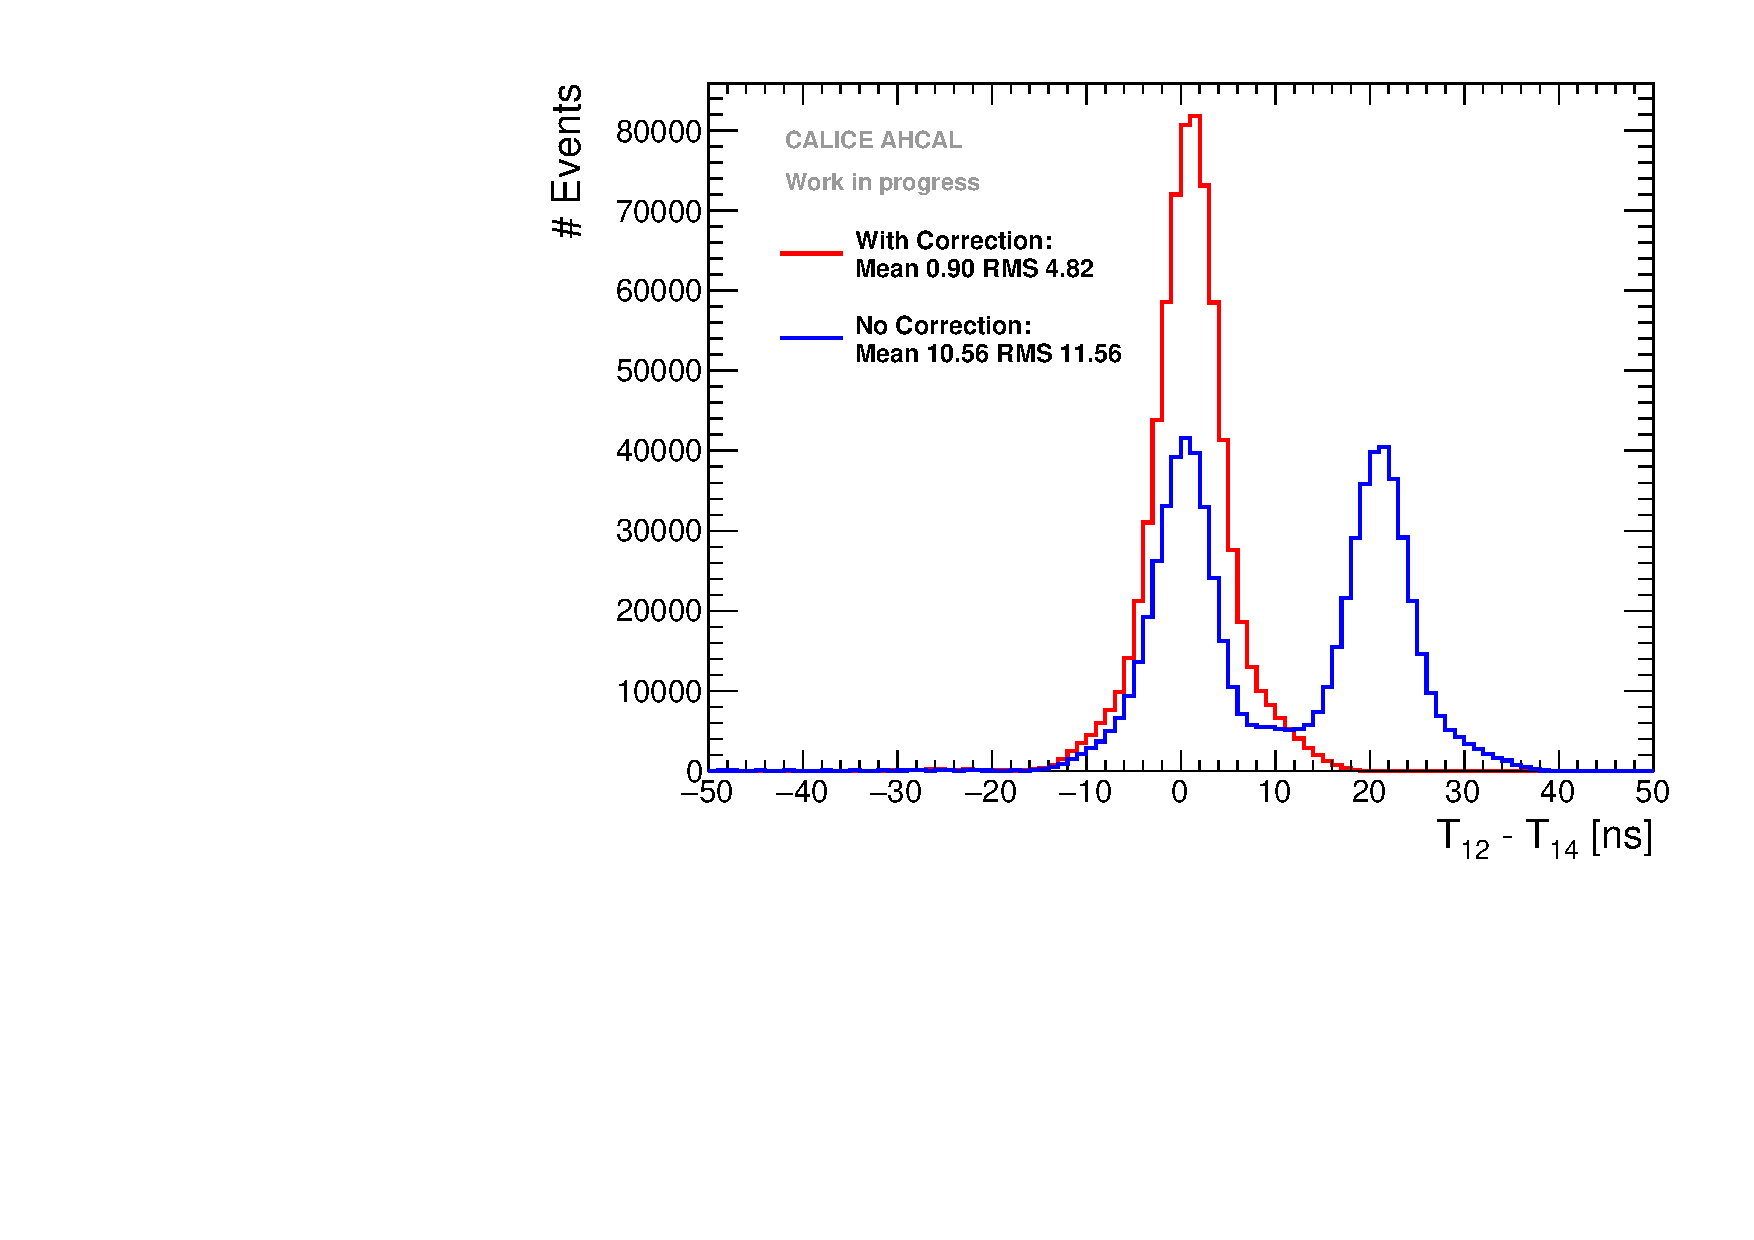
\includegraphics[width=1\linewidth]{fig/T0_Resolution_5.pdf}
		\caption{} \label{fig:T0Corr}
	\end{subfigure}
	\hfill
	\begin{subfigure}[t]{0.49\textwidth}
		\centering
		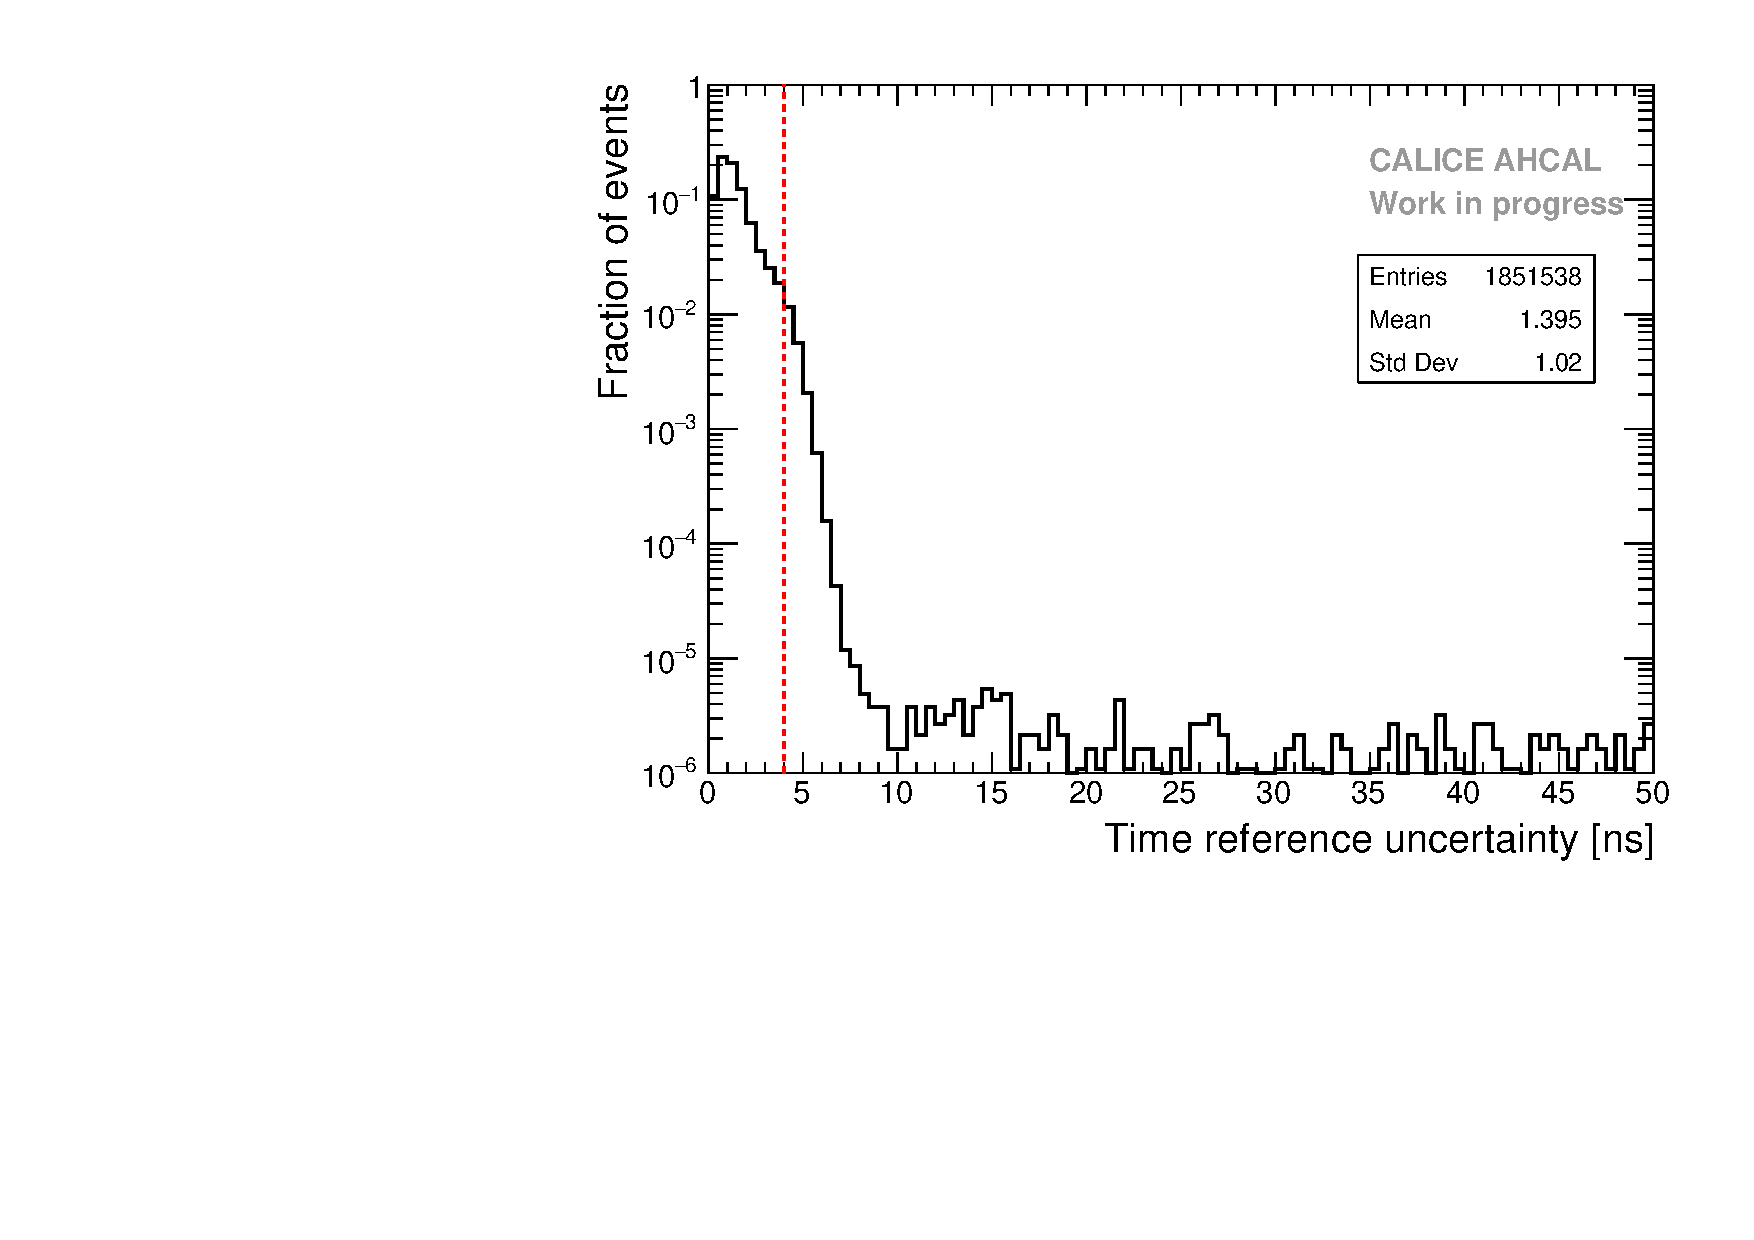
\includegraphics[width=1\linewidth]{fig/T0ReferenceError.pdf}
		\caption{} \label{fig:TRefErr}
	\end{subfigure}
	\caption{\subref{fig:T0Corr}) Time difference between the trigger channels before and after correction for T$_{12}$ and T$_{14}$. $\mu$ = 10.6 ns, RMS = 11.6 ns, $\mu_{corrected}$ = 0.9 ns, RMS$_{corrected}$ = 4.8 ns. The two visible peaks in blue are due to pedestal values being different dependent of the bunch-crossing parity. \subref{fig:TRefErr}) Distribution of the uncertainty $\sigma_{ref}$. The red line represents the cut of 4 ns.}
\end{figure}

Finally, the time reference is calculated as the mean of T$_{12}$, T$_{13}$ and T$_{14}$ per event. To reject events with a too large large time reference uncertainty, a cut of 4 ns on the time reference uncertainty is applied. The mean uncertainty of the time reference is around 1.30 ns as shown in figure \ref{fig:TRefErr}. This resolution from the time reference contributes to the final timing resolution obtained.

\subsection{Time delay correction}

The time reference of the trigger is delayed compared to the muon passing through the detector because of the length of cables and the trigger electronics logic. Therefore, the time offset of the time reference is determined from data. Muons are quasi-instantaneous particles thus the time of the first hit distribution for each channel, memory cell and BXID should peak at 0 ns.

\begin{figure}[htbp!]
	\centering
	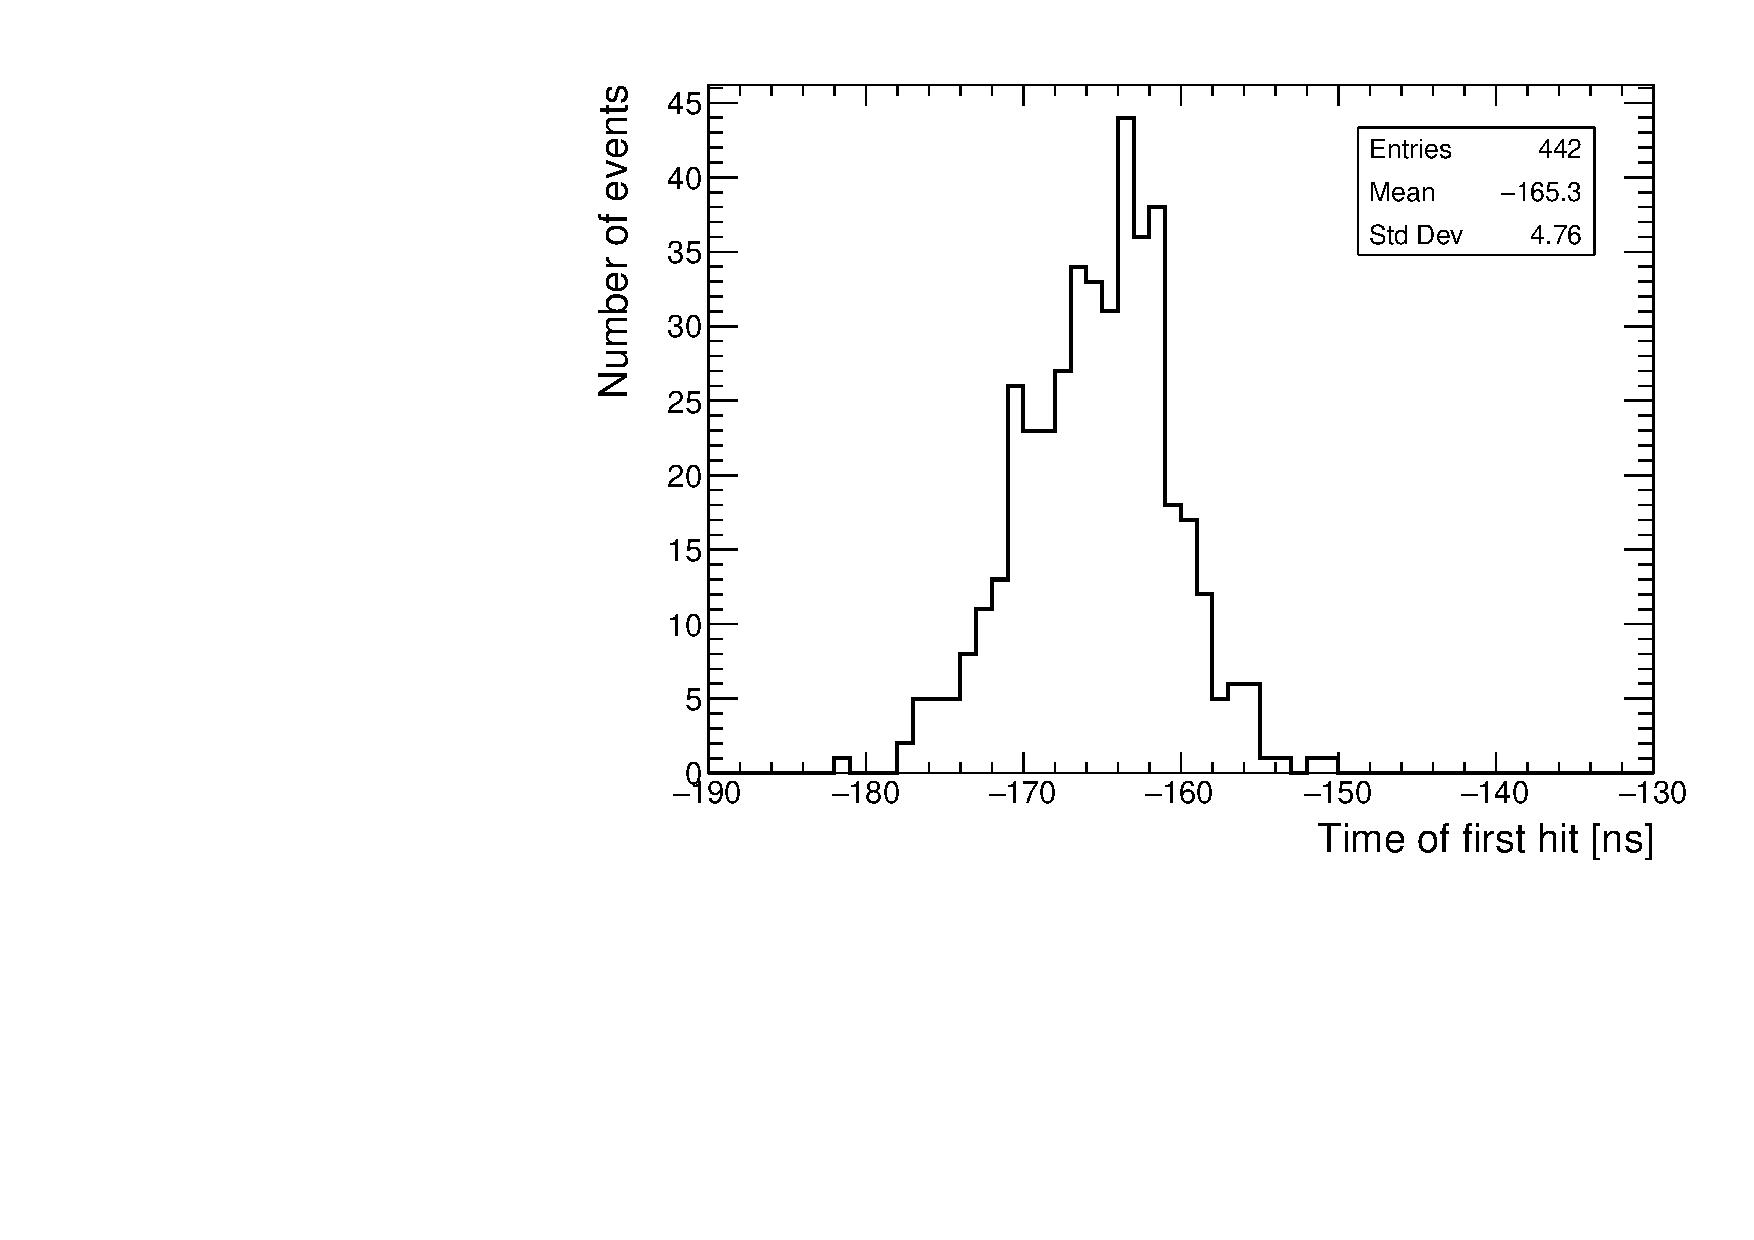
\includegraphics[width=0.6\textwidth]{fig/Timing_Chip236_Chn21_Mem01_BXID1_withOffset.pdf}
	\caption{Time of first hit distribution for a single channel (Chip 236, Chn 21, Mem 01, BXID 1). An offset of -165.2 ns is determined for this channel.}\label{fig:TimeChnwithOffset}
\end{figure}

A shifting procedure of the time of the hit relative to the time reference for each channel, memory-cell and BXID parity is performed. This is done to take into account the delay time of the trigger due to cabling and the trigger electronics as well as possible differences in channel pedestals. Only memory-cells containing more than 100 events are considered. The histogram range of the time of the hit relative to the time reference is reduced iteratively until the RMS of the distribution is under 10 ns. This value was chosen because it corresponds to more than 3 sigma of the time reference uncertainty. The mean of the histogram is then used as the time offset value. An example of a single channel is shown in figure \ref{fig:TimeChnwithOffset}.

In total, 21040 individual offsets are extracted from data. The mean value of the time offset is around -150 ns which is around the expected value considering the cabling length and the trigger logic delay.

\subsection{Non-linearity correction}

The time calibration relies on the linearity of the TDC voltage ramp in the \textit{SPIROC2B}. However, this assumption is not entirely reliable as described in \cite{Hartbrich2011, Brianne2012}. The voltage slope shows a slight kink around the middle thus leading to a non-linear ramp. For this, a correction of the non-linearity is applied. By investigating the time of the first hit for each chip and BXID parity as a function of the TDC value of the hit, the shape of the graph indicates how reliable is the assumption of a linear ramp. If the ramp would be perfectly linear, one would obtain a flat graph. To correct for the non-linearity of the ramp, a $2^{nd}$ order polynomial is used. A example for a typical chip is shown in figure \ref{fig:NLCorr}. The non-linearity correction results in an improvement in the timing resolution (RMS) of the AHCAL by about 5.1\% as shown in figure \ref{fig:TimingNLCorr}.

\begin{figure}[htbp!]
	\begin{subfigure}[t]{0.49\textwidth}
		\centering
		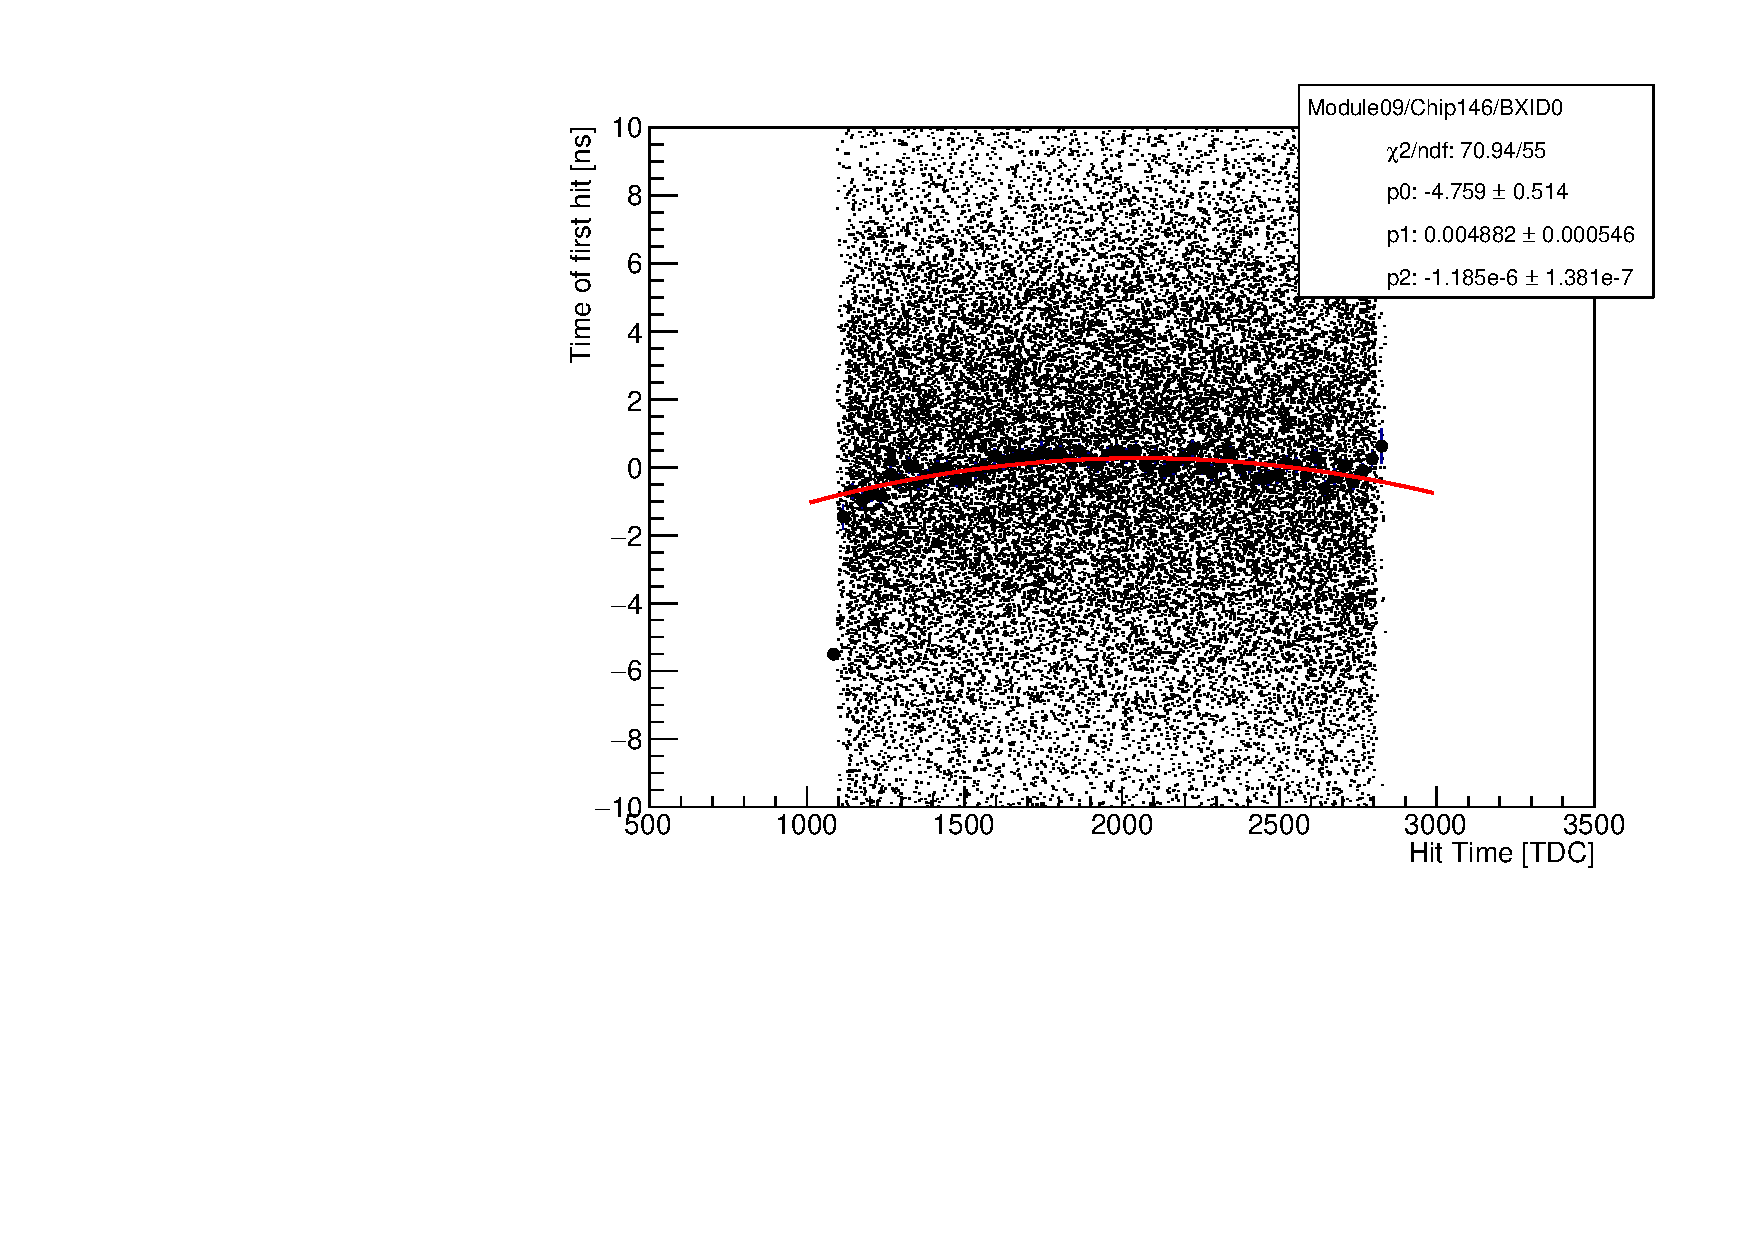
\includegraphics[width=1\linewidth]{fig/LinearityCorrection_Module09_Chip146_BXID0.pdf}
		\caption{} \label{fig:NLCorr}
	\end{subfigure}
	\hfill
	\begin{subfigure}[t]{0.49\textwidth}
		\centering
		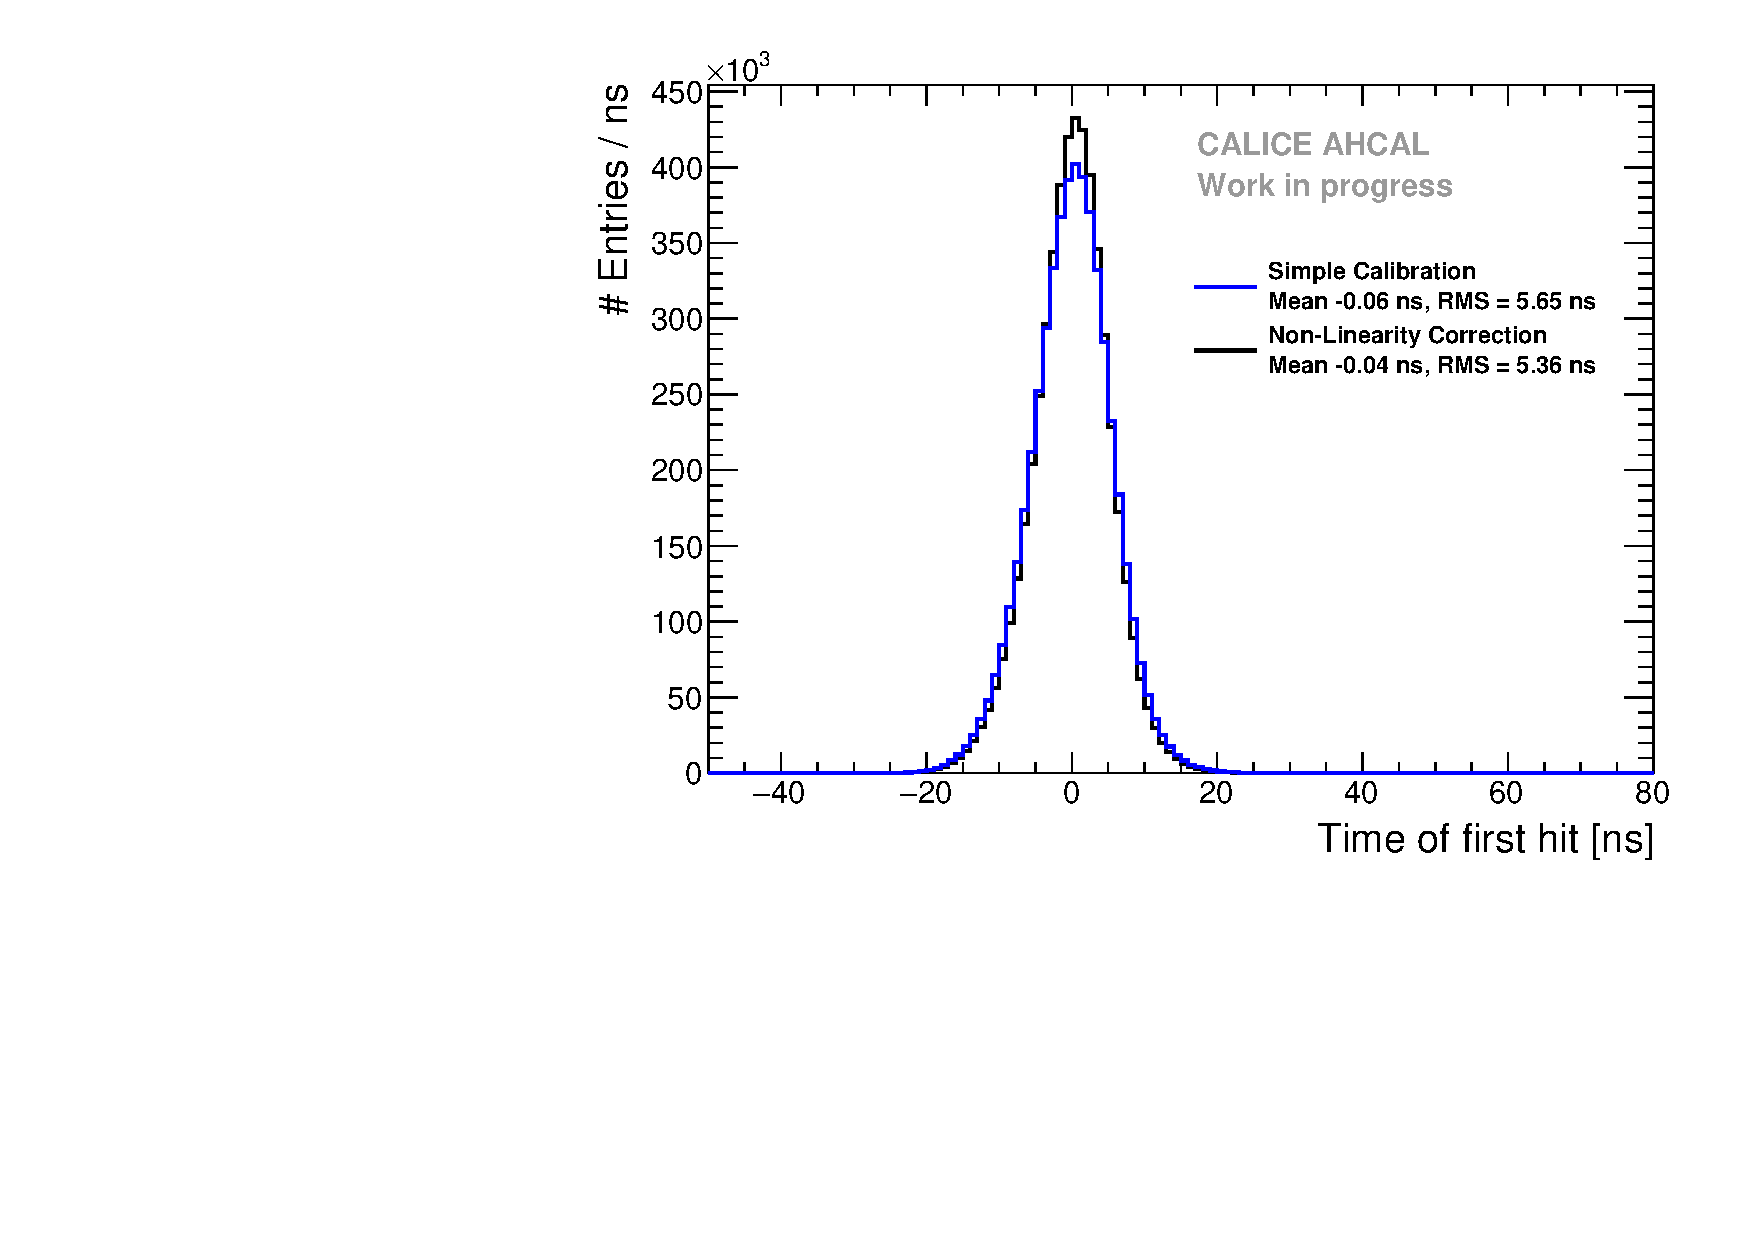
\includegraphics[width=1\linewidth]{fig/Timing_AHCAL_LinCorrection.pdf}
		\caption{} \label{fig:TimingNLCorr}
	\end{subfigure}
	\caption{\subref{fig:NLCorr}) Quadratic fit of chip 146 (BXID even) on layer 9. The graph is slightly curved showing that this chip presents a non-linear TDC ramp. $\chi^{2}$/ndf = 1.29. \subref{fig:TimingNLCorr}) Time of the first hit distribution before and after the non-linearity correction. The correction results in an improvement of around 5\% on the RMS of the distribution.}
\end{figure}

\subsection{Time-walk correction}
\label{sec:TWCorr}

The time-walk effect is due to the presence of an energy threshold that induces a time shift between a small amplitude signal and a high amplitude signal. Small amplitude signals will systematically trigger at a later time than high amplitude signals for a shaper that makes the signals peak at the same time. A time correction is determined by looking at the time of the first hit as a function of the amplitude of the hit as shown in figure \ref{fig:time_walk}. This may be particularly relevant for late energy depositions in hadron showers that comes generally from neutrons depositing little energy in the calorimeter. An improvement of around 3\% is achieved on the time resolution of the AHCAL as shown in figure \ref{fig:Timing_AllCorr}.

\begin{figure}[htbp!]
	\begin{subfigure}[t]{0.49\textwidth}
		\centering
		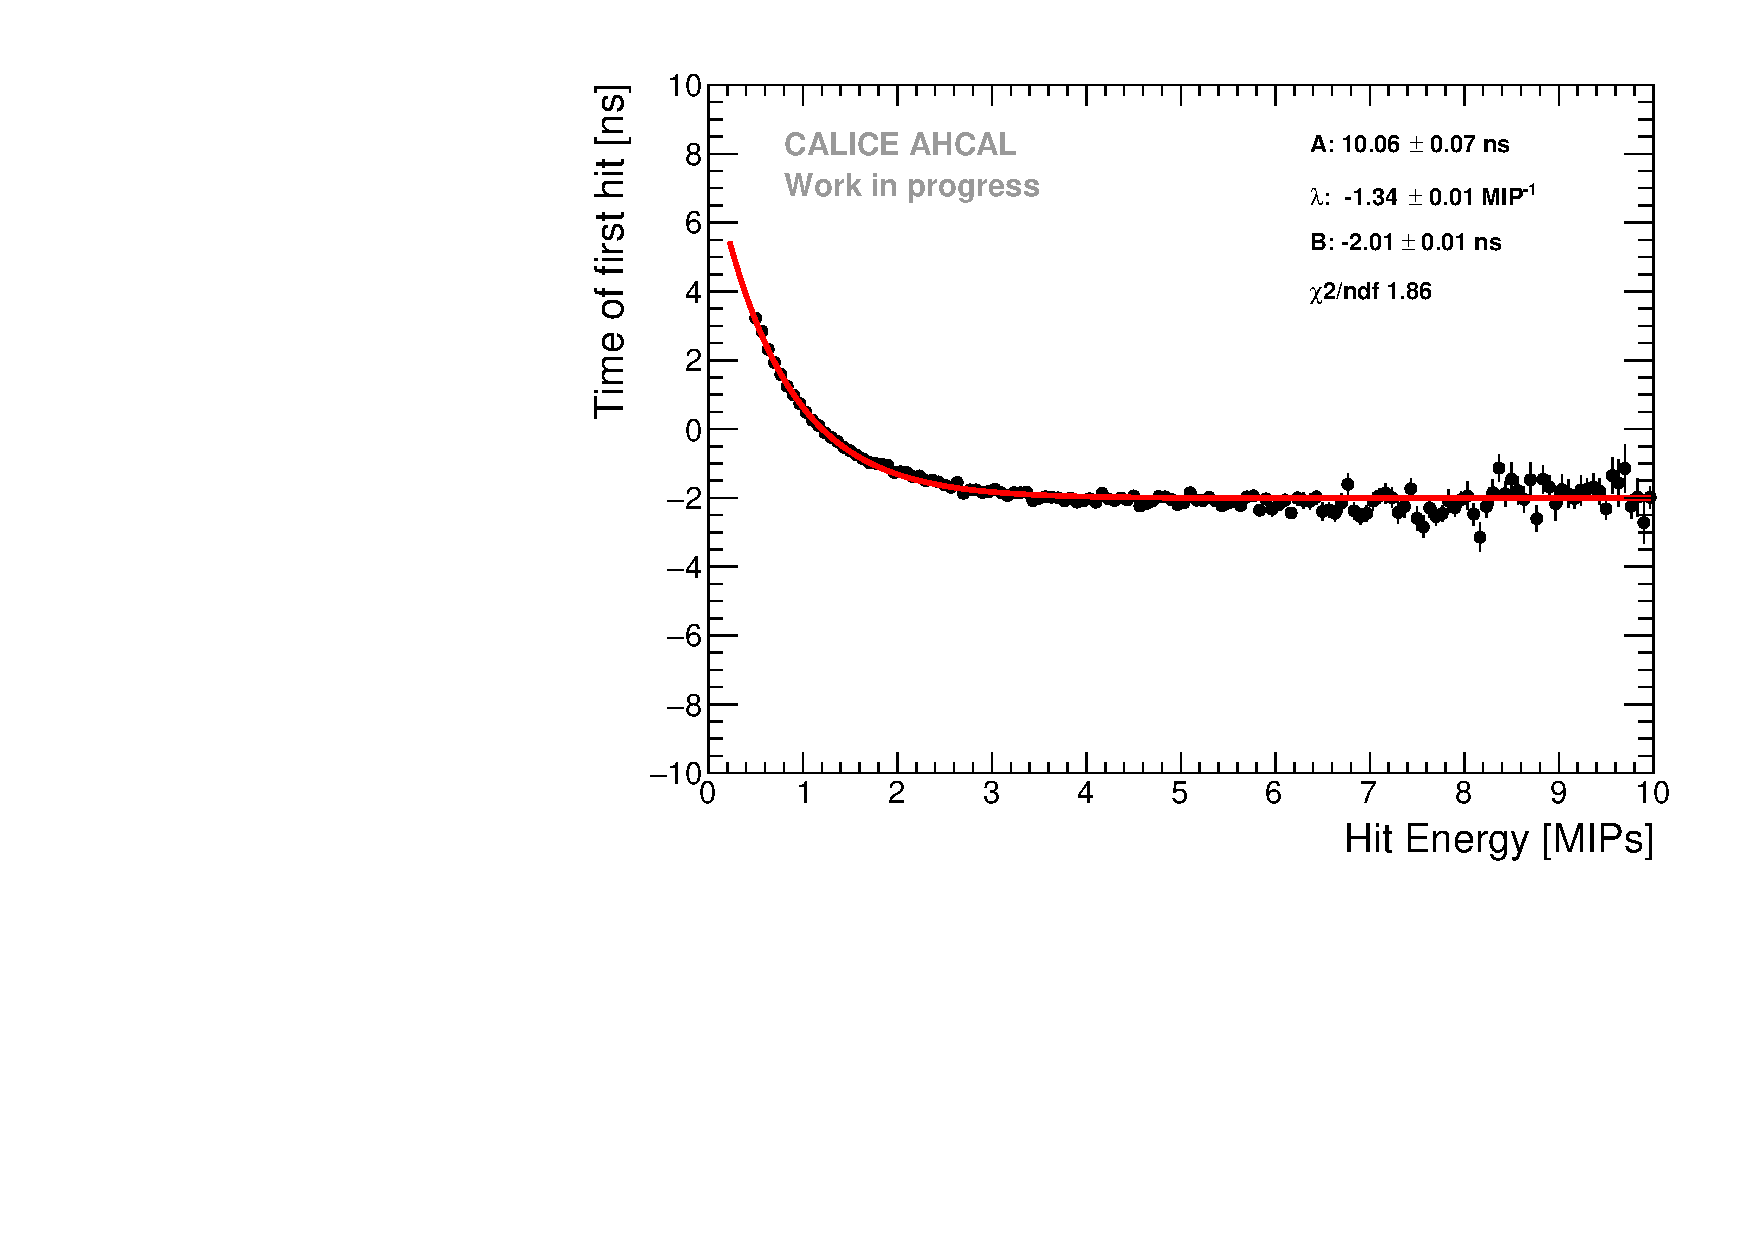
\includegraphics[width=1\linewidth]{fig/TimeWalkProfile.pdf}
		\caption{} \label{fig:time_walk}
	\end{subfigure}
	\hfill
	\begin{subfigure}[t]{0.49\textwidth}
		\centering
		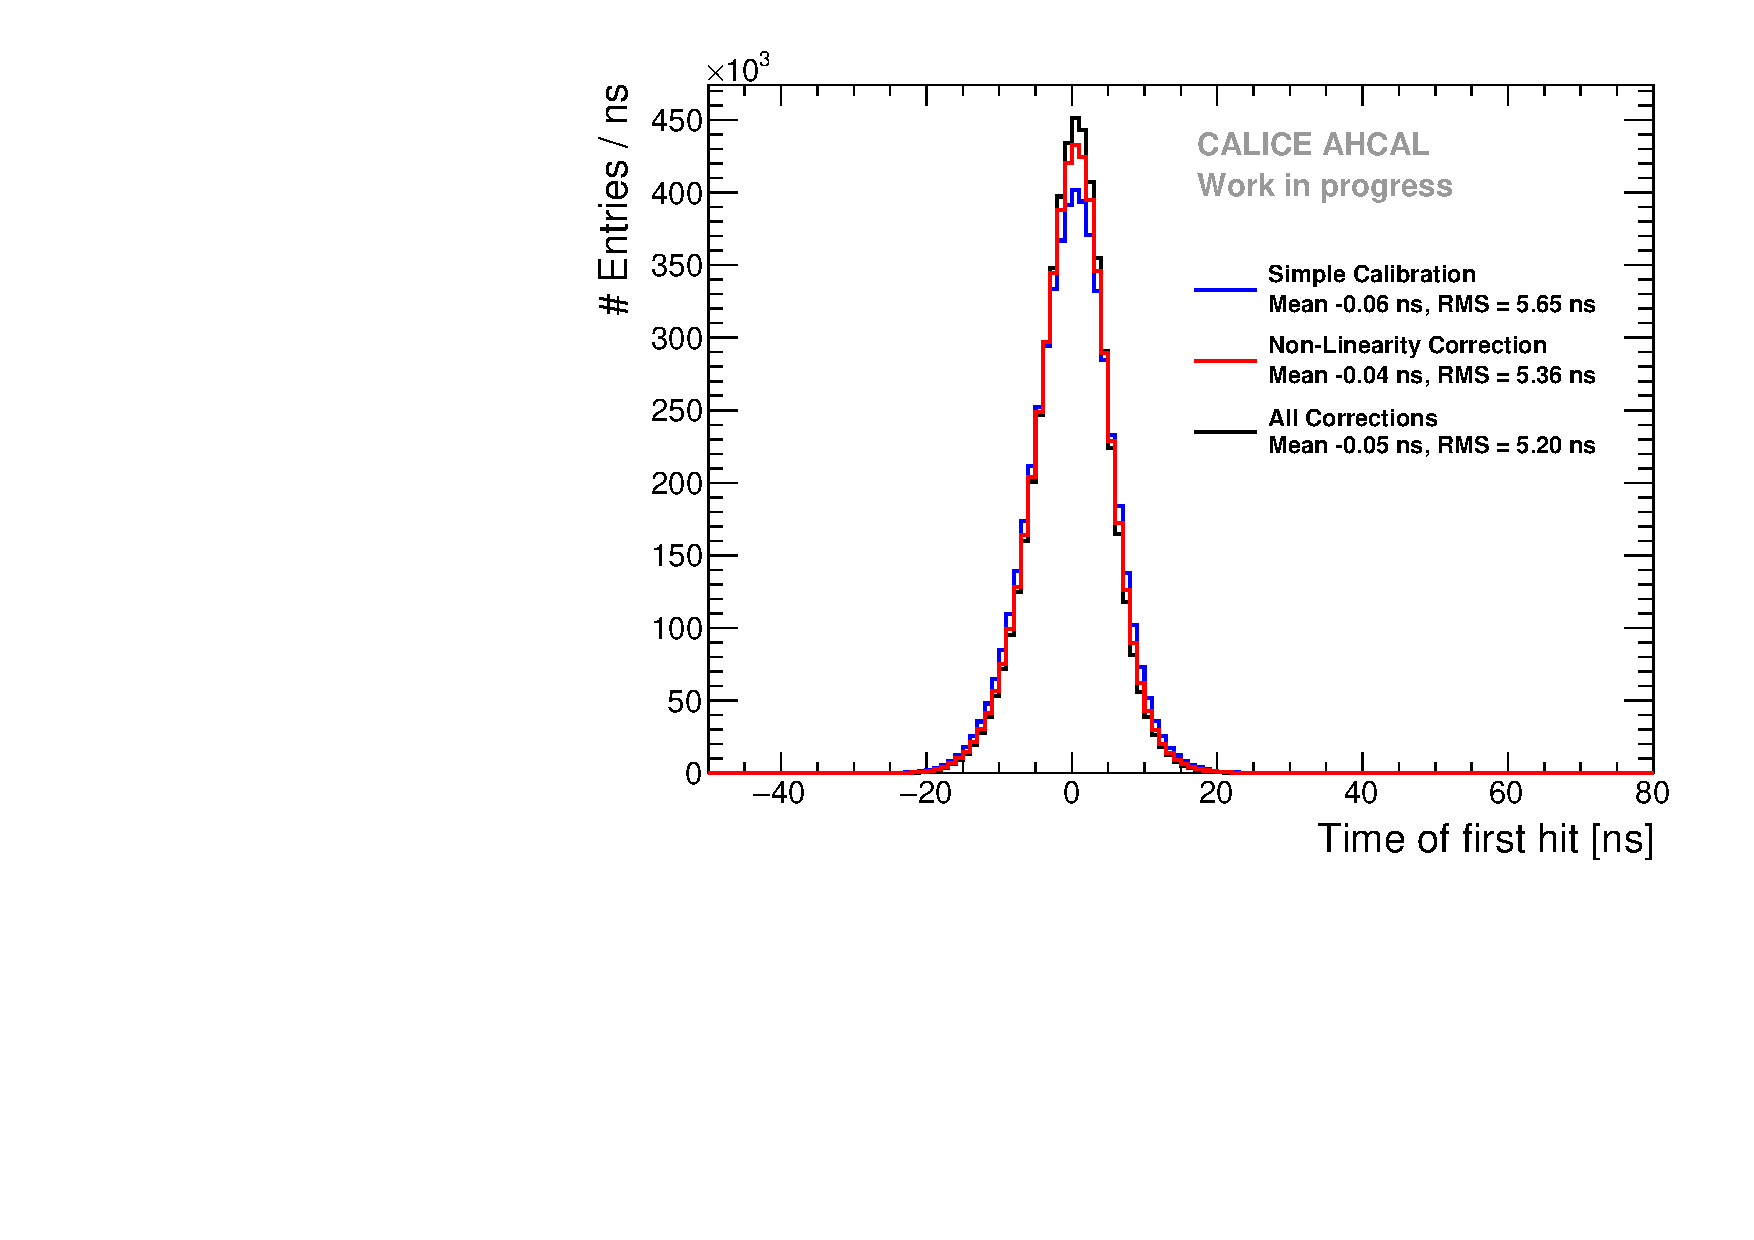
\includegraphics[width=1\linewidth]{fig/Timing_AHCAL_AllCorrection.pdf}
		\caption{} \label{fig:Timing_AllCorr}
	\end{subfigure}
	\caption{\subref{fig:time_walk}) Time of first hit as a function of the hit energy. A difference up to 6 ns is seen between small and large amplitudes. Time-walk correction extracted from data. The fit function is of the form $\text{A} \times e^{-\lambda{}x} + \text{B}$. \subref{fig:Timing_AllCorr}) Time of the first hit distribution before and after the time-walk correction. The correction results in an improvement of around 3\% on the RMS of the distribution.}
\end{figure}

\subsection{Number of triggered channel in a chip correction}
\label{sec:NumberTrigger}

After the time calibration, electrons show a significantly worse time resolution. This could be traced back to events where there are many channels that are triggered in the same chip. The mean time of first hit as a function of the number of triggered channels over 0.5 MIP in a chip is shown in figure \ref{fig:nhits_profile}. A time shift up to 20-40 ns can be seen depending on the number of triggered channels in a chip. The cause of the observed effect is most likely due to an element in the chip called a \textit{delay box} that gets unstable with a high charge going through the chip. This chip element is responsible for the hold signal of the TDC ramp in the chip. The hold signal is delayed, and thus a higher TDC ramp value than the one expected is sampled.

\begin{figure}[htbp!]
	\begin{subfigure}[t]{0.49\textwidth}
		\centering
		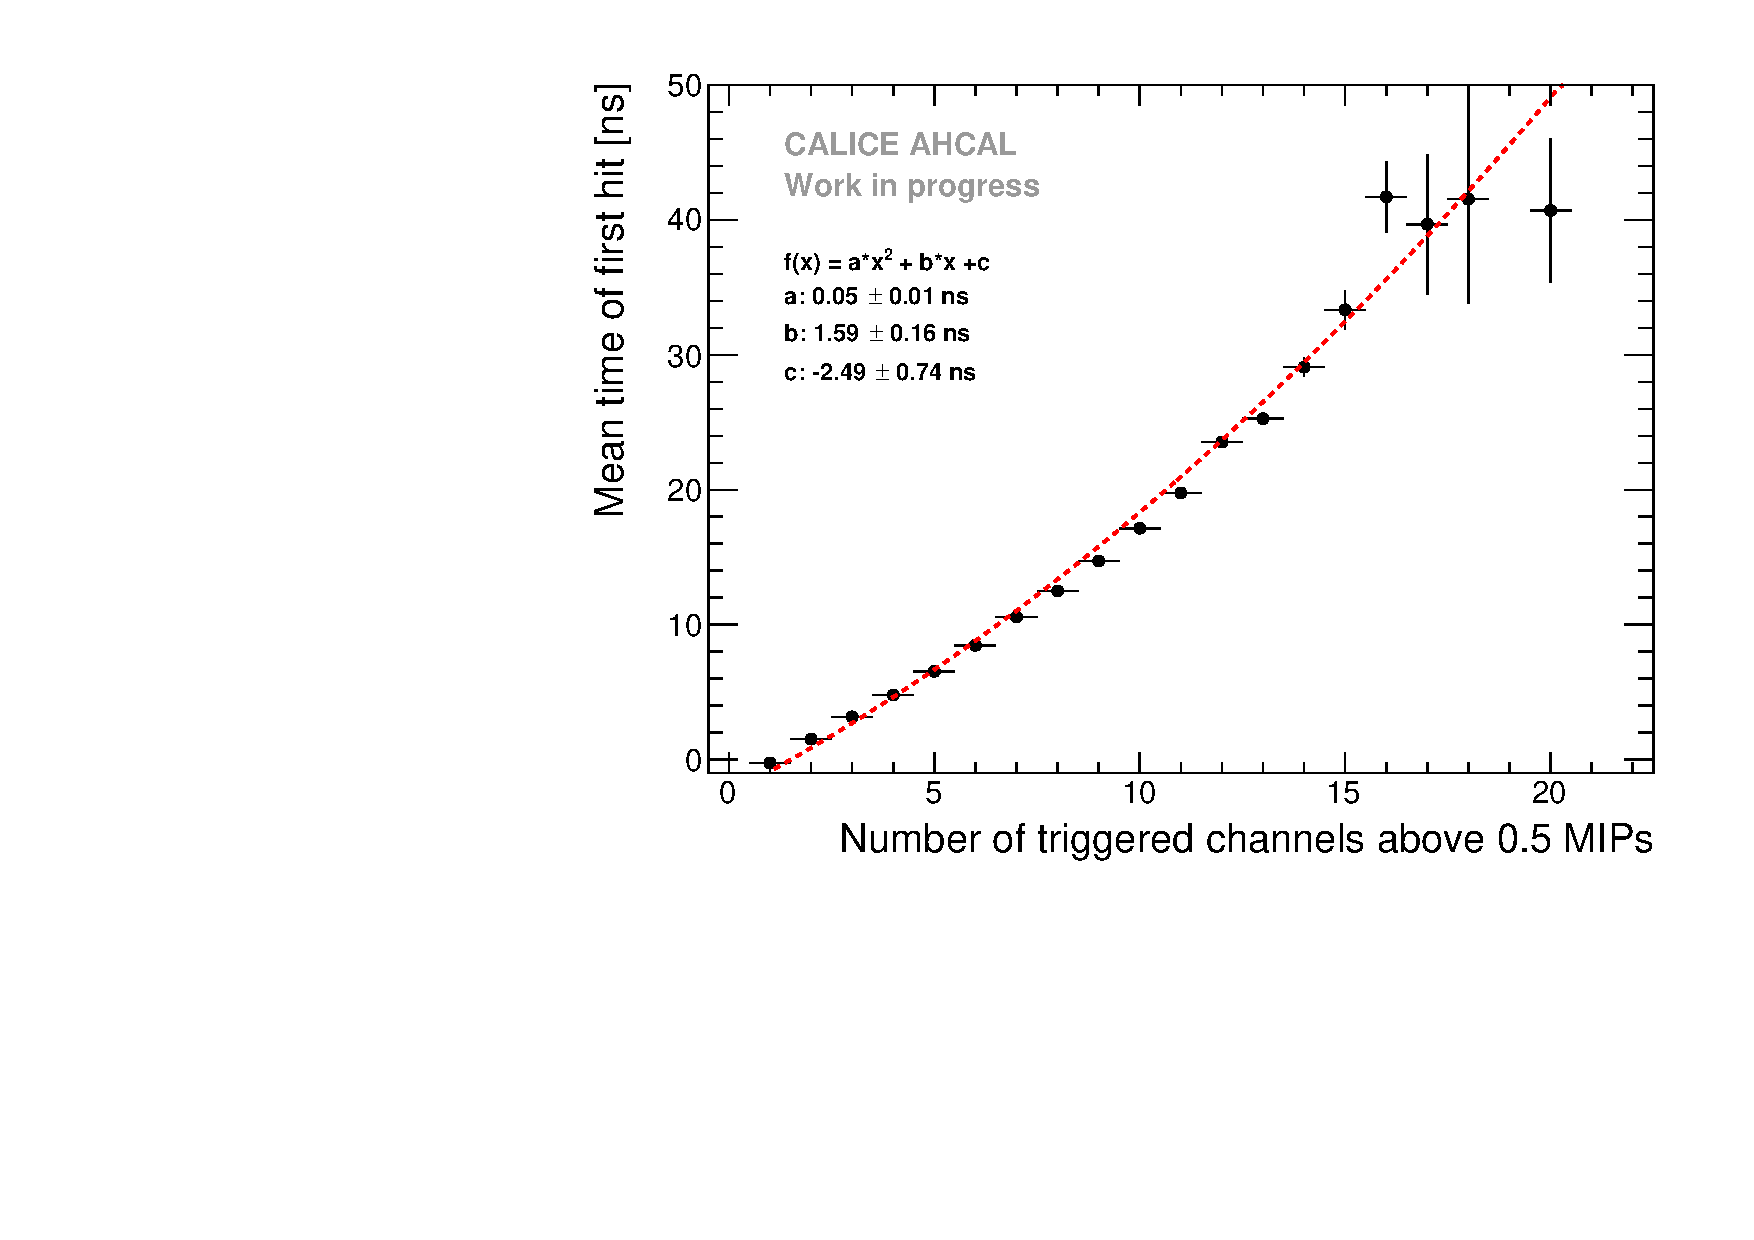
\includegraphics[width=1\linewidth]{fig/NumberHits_Dependance_AllEnergies.pdf}
		\caption{} \label{fig:nhits_profile}
	\end{subfigure}
	\hfill
	\begin{subfigure}[t]{0.49\textwidth}
		\centering
		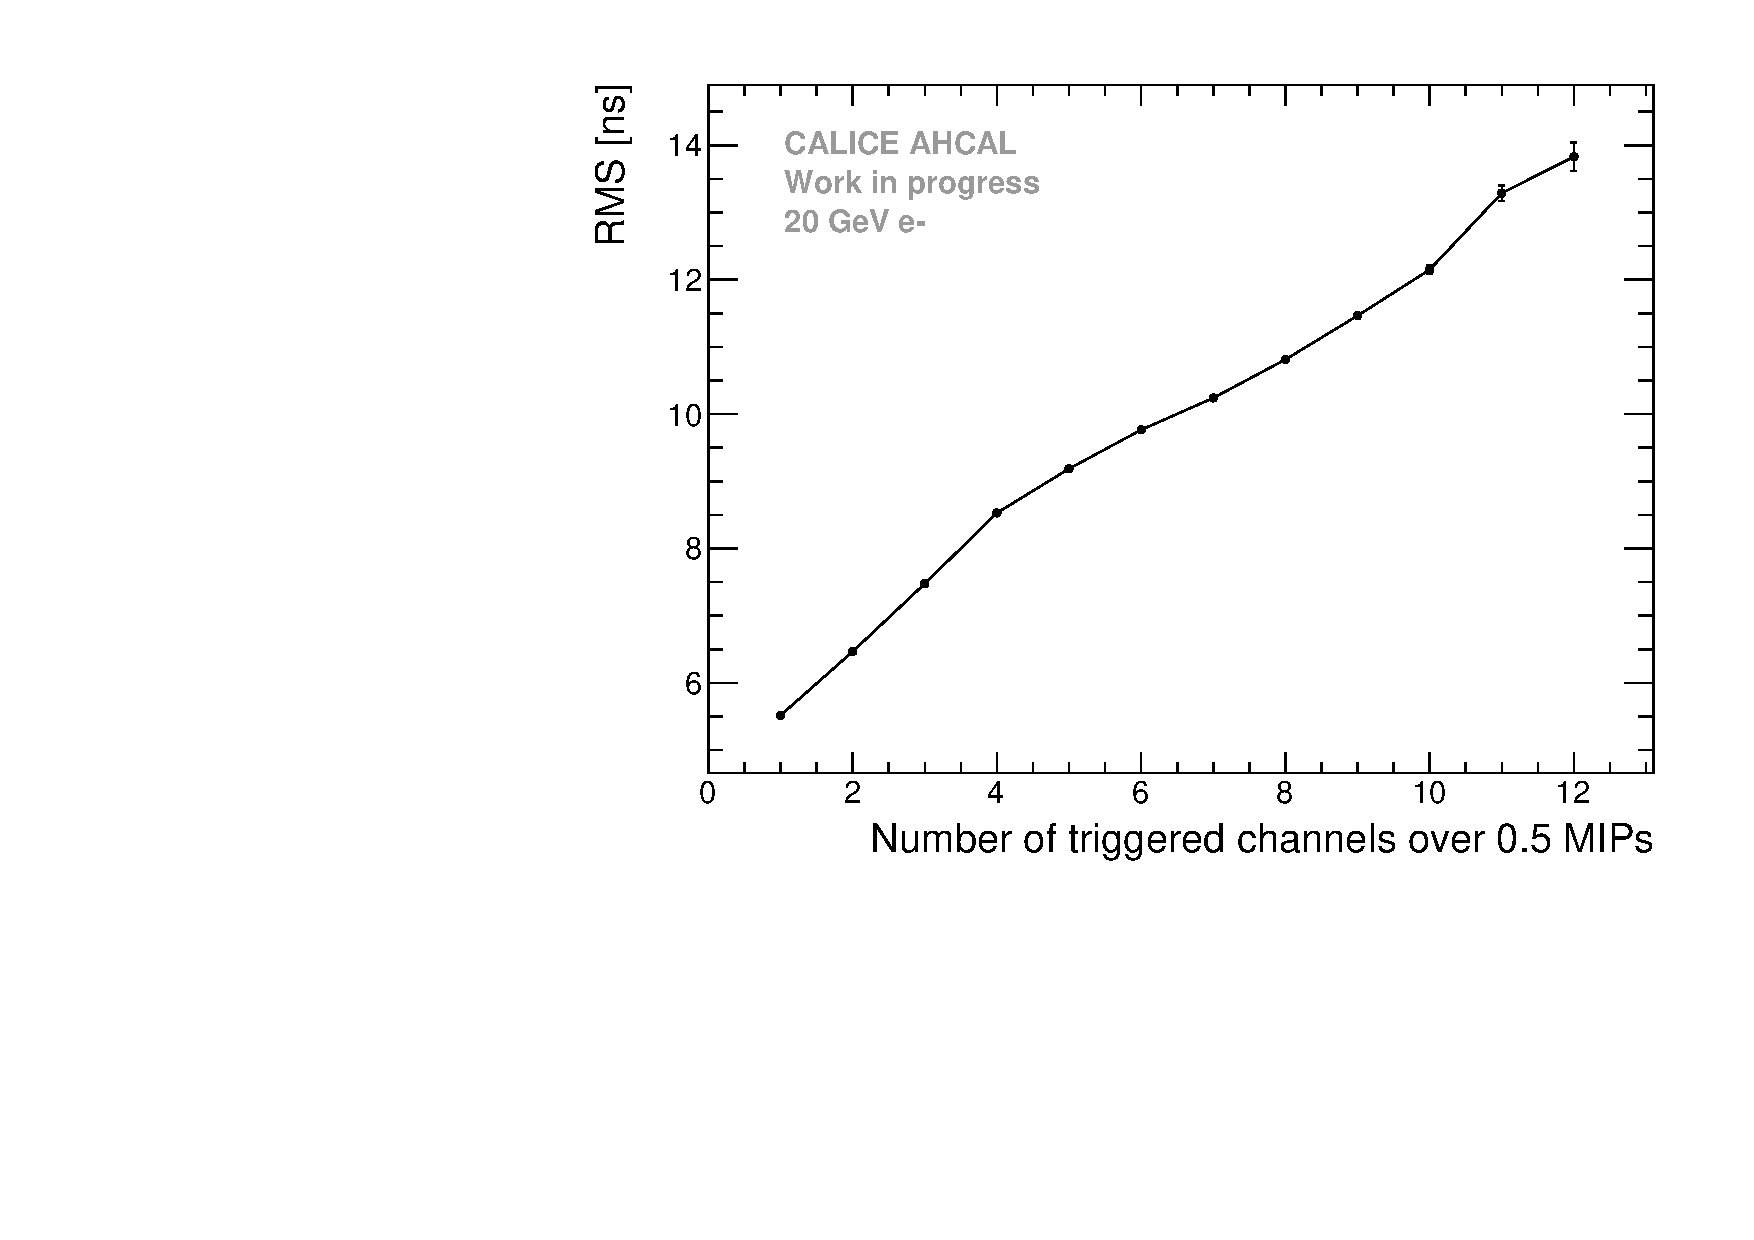
\includegraphics[width=1\linewidth]{fig/ParametrisationPedestalShift_20GeV.pdf}
		\caption{} \label{fig:nhits_RMS_profile}
	\end{subfigure}
	\caption{\subref{fig:nhits_profile}) Mean time of the first hit as a function of the number of triggered channels above 0.5 MIP in a chip. The mean time shift upwards with the increase of triggers leading to large tails in the time distribution. A second order polynomial fit is done for the time correction shown by the red dashed line. \subref{fig:nhits_RMS_profile}) RMS of the time distribution for 20 GeV electrons as a function of the number of triggered channels in a chip.}
\end{figure}

Not only this effect shifts the mean time of the hit but as well it increase the RMS of the time distribution as shown in figure \ref{fig:nhits_RMS_profile} for 20 GeV electrons. In order to determine a reliable time correction, the time correction parameters are determined combining all the electron data. This effect may be chip-dependent and the parameters for the correction may differ from chip to chip. However, the limited amount of data does not allow to determine a correction function for each chip. Therefore, a global function is used to correct the time in the data. This effect is parametrized in simulation as explained in section \ref{sec:GeoDigi}.

\section{Results}

\subsection{Systematic uncertainties}

Systematic uncertainties need to be evaluated in order to perform a significant assessment of differences observed between data and simulations. Several possible sources were identified:

\begin{itemize}
	\item Non-Linearity correction: A non-linearity correction is determined from data with a limited accuracy lead to a systematic uncertainty. The residuals of the correction give a systematic uncertainty at the level of 0.2 ns.
	\item Time walk correction: Similarly to the non-linearity correction, the systematic uncertainty obtained from the residuals of the time walk correction in data is in the order of 0.2 ns.
	\item Number of triggered channels correction: The correction in data for the number of triggered channels over 0.5 MIP in a chip results in a residual on the mean time of the first hit. The uncertainty for the mean time of the hit is computed per bins of energy, radius and depth by weighting according to the fraction of hits in the regions of 0-5, 5-12 and over 12 number of hits per chip with the errors of 2, 5 and 7 ns respectively. The systematic uncertainty varies between 1.8 to 3 ns. For the time of first hit distribution, a systematic uncertainty is applied bin-by-bin for electrons and pions in the region of -30 ns to 30 ns. Outside of this region, a systematic error of 50\% is taken. This systematic uncertainty is the most dominant over all other uncertainties.
	\item AHCAL energy scale: The energy scale of the AHCAL was determined using the muon dataset. A systematic uncertainty on the MIP scale of around 3.6\% was derived by dividing the muon sample in odd and even run numbers and by looking at the average spread of the fitted MIP value for both subsamples. This is converted to an uncertainty in time using the mean time of first hit as a function of the hit energy using the QGSP\_BERT\_HP physics list. At 0.5 MIP, this results in an uncertainty of 0.1 ns. For hits above 1 MIP, the uncertainty is below 0.05 ns.
	\item Global time smearing parameters: A global time smearing parametrization is used from muon data to smear the time in simulation. A bin-by-bin systematic uncertainty is applied to the time of first hit distribution in simulation to take into account the difference with a layer-wise time smearing parametrization.
	\item Number of triggered channels in a chip parametrization: A smearing parametrization of the width of the time distribution as a function of the number of triggered channels in a chip is obtained from electron data. An error band on the width was obtained by comparing all electron energies as explained. This is applied to simulation for systematics.
	\item Determination of the offset to $t=0$: For simulation, the time shift per layer is calculated using a time of flight correction $T_{of} = \frac{z_{layer}}{c}$ with $c$ the speed of light and $z_{layer}$ the z position of a layer. For this, an uncertainty of 3 mm corresponding to the scintillator thickness is taken in z corresponding to 0.01 ns uncertainty in timing.
	\item Cross-talk: No measurement for optical cross-talk between tiles is available and from previous measurements, it varies between 10\% and 18\%. The cross-talk value induces a different number of hits in the detector thus has an impact on the width of the time of first hit distribution. The variation of this parameter in the simulation for the layers 4 to 10 is used for systematics.
	\item Absolute number of events: In the pion data, some possible contamination from multi-particle events may be present still after the selection. Thus, the number of true pion events is not known. The cluster time rejection method (see section \ref{sec:pionsel}) rejects up to 1\% of events in the data. A conservative uncertainty of 10\% on the data normalization is assigned when comparing data to simulation for the time of first hit distribution.
\end{itemize}

The systematic uncertainties are added in quadrature for the full systematic uncertainty assuming no correlation between uncertainties. For the mean time of the first hit as a function of the hit energy and as a function of the hit distance to the shower center of gravity, the systematic uncertainty is resulting at 0.3 ns for muons and 1.09 ns for electrons and pions. The table \ref{table:time_syst} sums up the systematic uncertainties used in the analysis.

\begin{table}[htb!]
	\centering
	\caption{Summary of systematic uncertainties.}
	\label{table:time_syst}
	\begin{tabular}{@{} lc @{}}
		\toprule
		\multicolumn{1}{c}{Uncertainty source} & Full uncertainty \\
		\midrule
		Non-linearity correction & 0.2 ns \\
		Time-walk correction & 0.2 ns \\
		Number of triggered channels correction & 1.8 - 3 ns / bin-wise (e/$\pi$)\\
		Energy Scale & 0.05-0.1 ns \\
		Time of flight offset & 0.01 ns (MC) \\
		Cross-talk parameter & 10-18\% (MC)\\
		Global time smearing parameters & bin-wise (MC)\\
		Number of triggered channels in a chip parametrization & bin-wise (MC)\\
		Multi-particle events & 10\% ($\pi$) \\
		\midrule
		\midrule
		\multicolumn{2}{c}{Systematics combined} \\
		\midrule
		data-MC ToFH distribution & bin-wise (e) - bin-wise + 10\% ($\pi$) \\
		data-MC vs hit energy & 0.3 ns ($\mu$) - 1.8 to 3 ns (e/$\pi$)\\
		data-MC vs hit distance to shower CoG & 0.3 ns ($\mu$) - 1.8 to 3 ns (e/$\pi$)\\
		data-MC vs hit depth & 0.3 ns ($\mu$) - 1.8 to 3 ns (e/$\pi$)\\
		\bottomrule
	\end{tabular}
\end{table}

\subsection{Timing of muon and electron beams}

Firstly, the comparison of the time of first hit distribution for muons between data and simulations is shown in figure \ref{fig:sim_data_muon}. The comparison shows that in the range of -20 ns to 20 ns, data and simulation agree well within the uncertainties. However, over 20 ns (and below -20 ns), the tails of the simulation are underestimated. This is due to the noise implementation in simulation that is not perfectly reproduced. In addition, the time of distribution has been checked layer-by-layer and compared to simulations. Similarly, the agreement between data and simulations is best in the range of -20 ns to 20 ns and the tails are not perfectly reproduced in simulation.

\begin{figure}[htbp!]
	\centering
	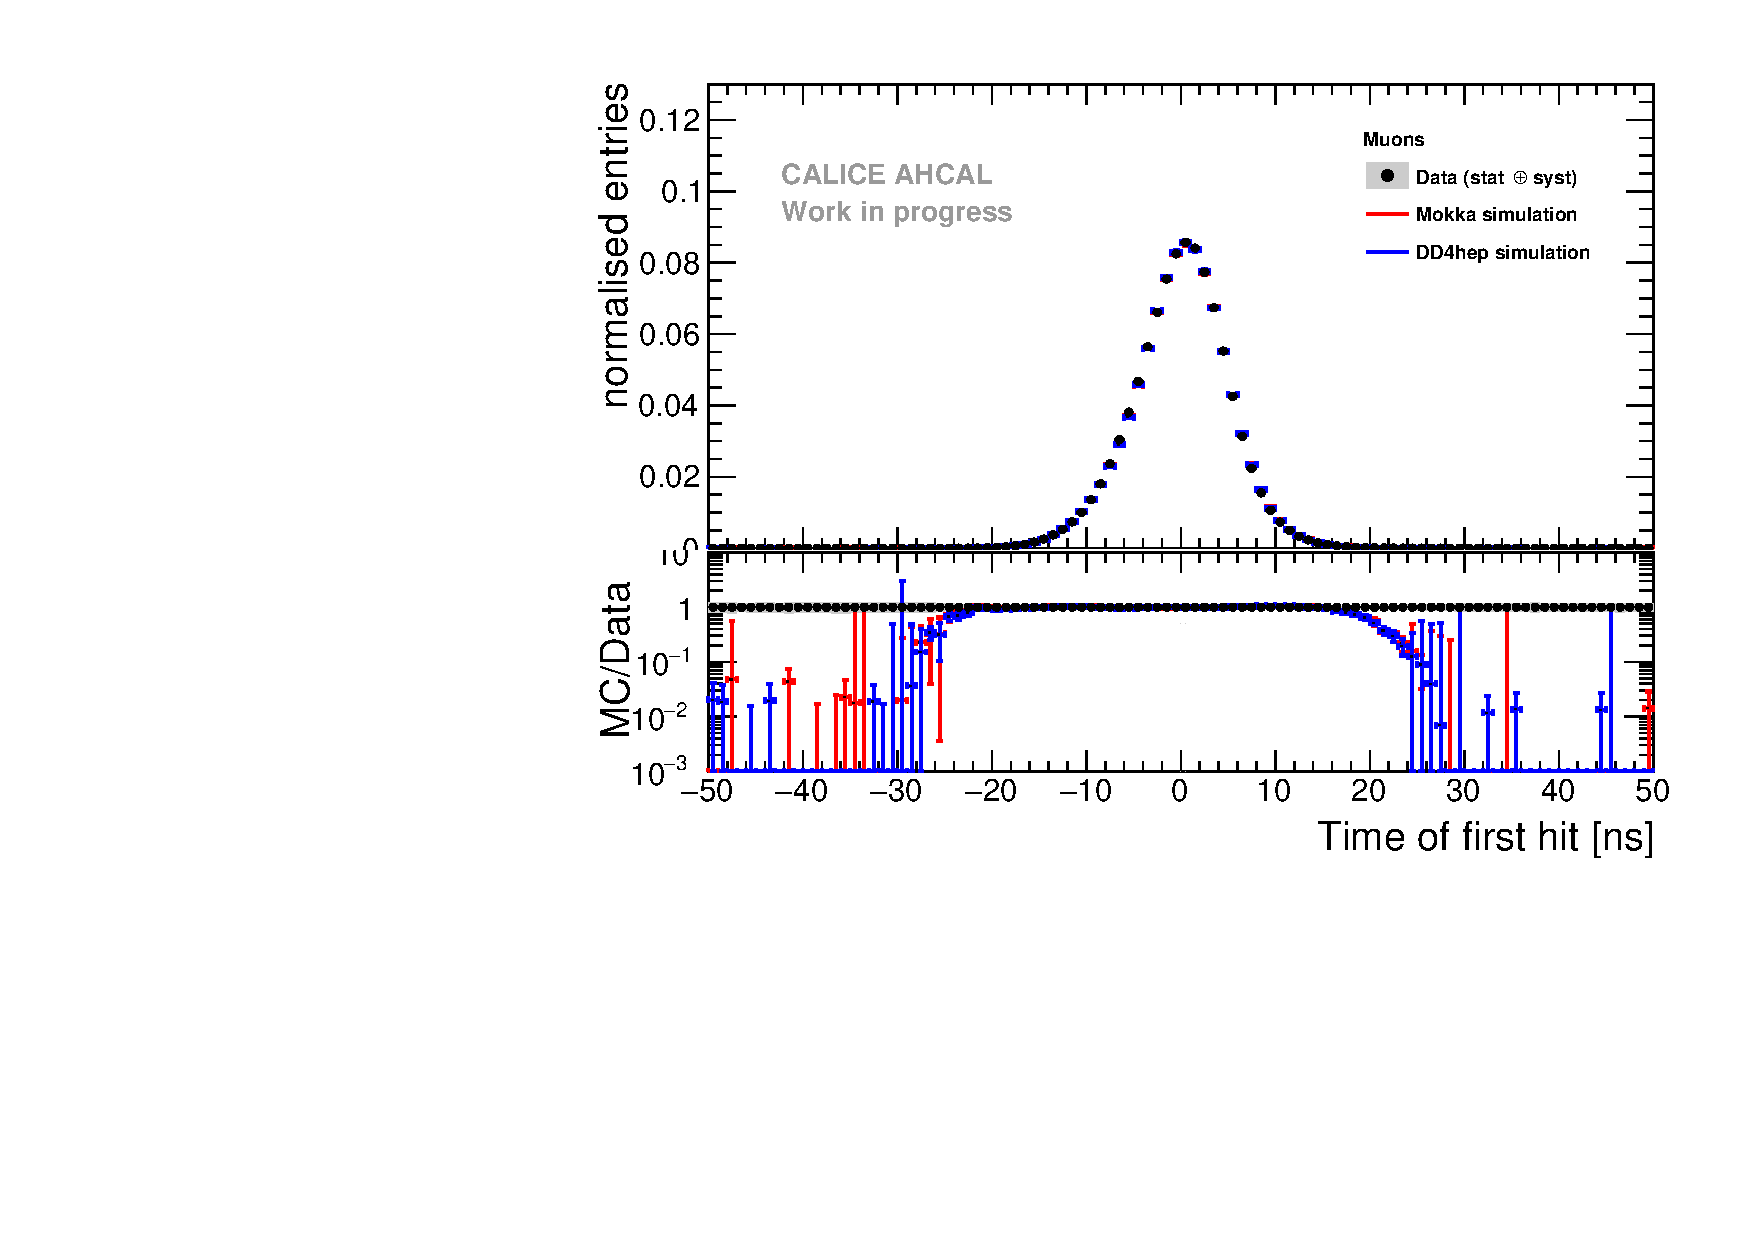
\includegraphics[width=0.6\textwidth]{fig/Comparison_MokkaDD4hepData_Muons.pdf}
	\caption{Time of first hit distribution for muons in data and simulation between -50 and 50 ns. The grey area represents the statistical uncertainty of the data. The error bars of the simulation are obtained by varying the cross-talk parameter between 10\% and 18\% and taking into account the error of a global time smearing parametrization.}
	\label{fig:sim_data_muon}
\end{figure}

Secondly, to further validate the time simulation, comparisons with electron data has been done. The figure \ref{fig:elec_sim_data_10GeV} shows the comparison of the time of first hit distribution for 10 GeV electrons in data and simulation. The simulation is systematically narrower than data. This is caused by the simulation having fewer hits in a chip than data which can be seen in figure \ref{fig:elec_sim_data_nHits_10GeV}. The simulation is generally 10\% to 20\% lower than data in the region of 6 to 10 hits per chip. Overall, the simulation describes well the data within statistical and systematic uncertainties in the central region of -30 ns to 30 ns for all energies. The large fluctuations in the simulation are due to the parametrization of the increase of the width. However, the description of the tails of the time of first hit distribution in the simulation are well underestimated. Like for muons, this is due to the description of the noise in the simulation that is not perfectly reproduced.

\begin{figure}[htbp!]
	\centering
	\begin{subfigure}[t]{0.49\textwidth}
		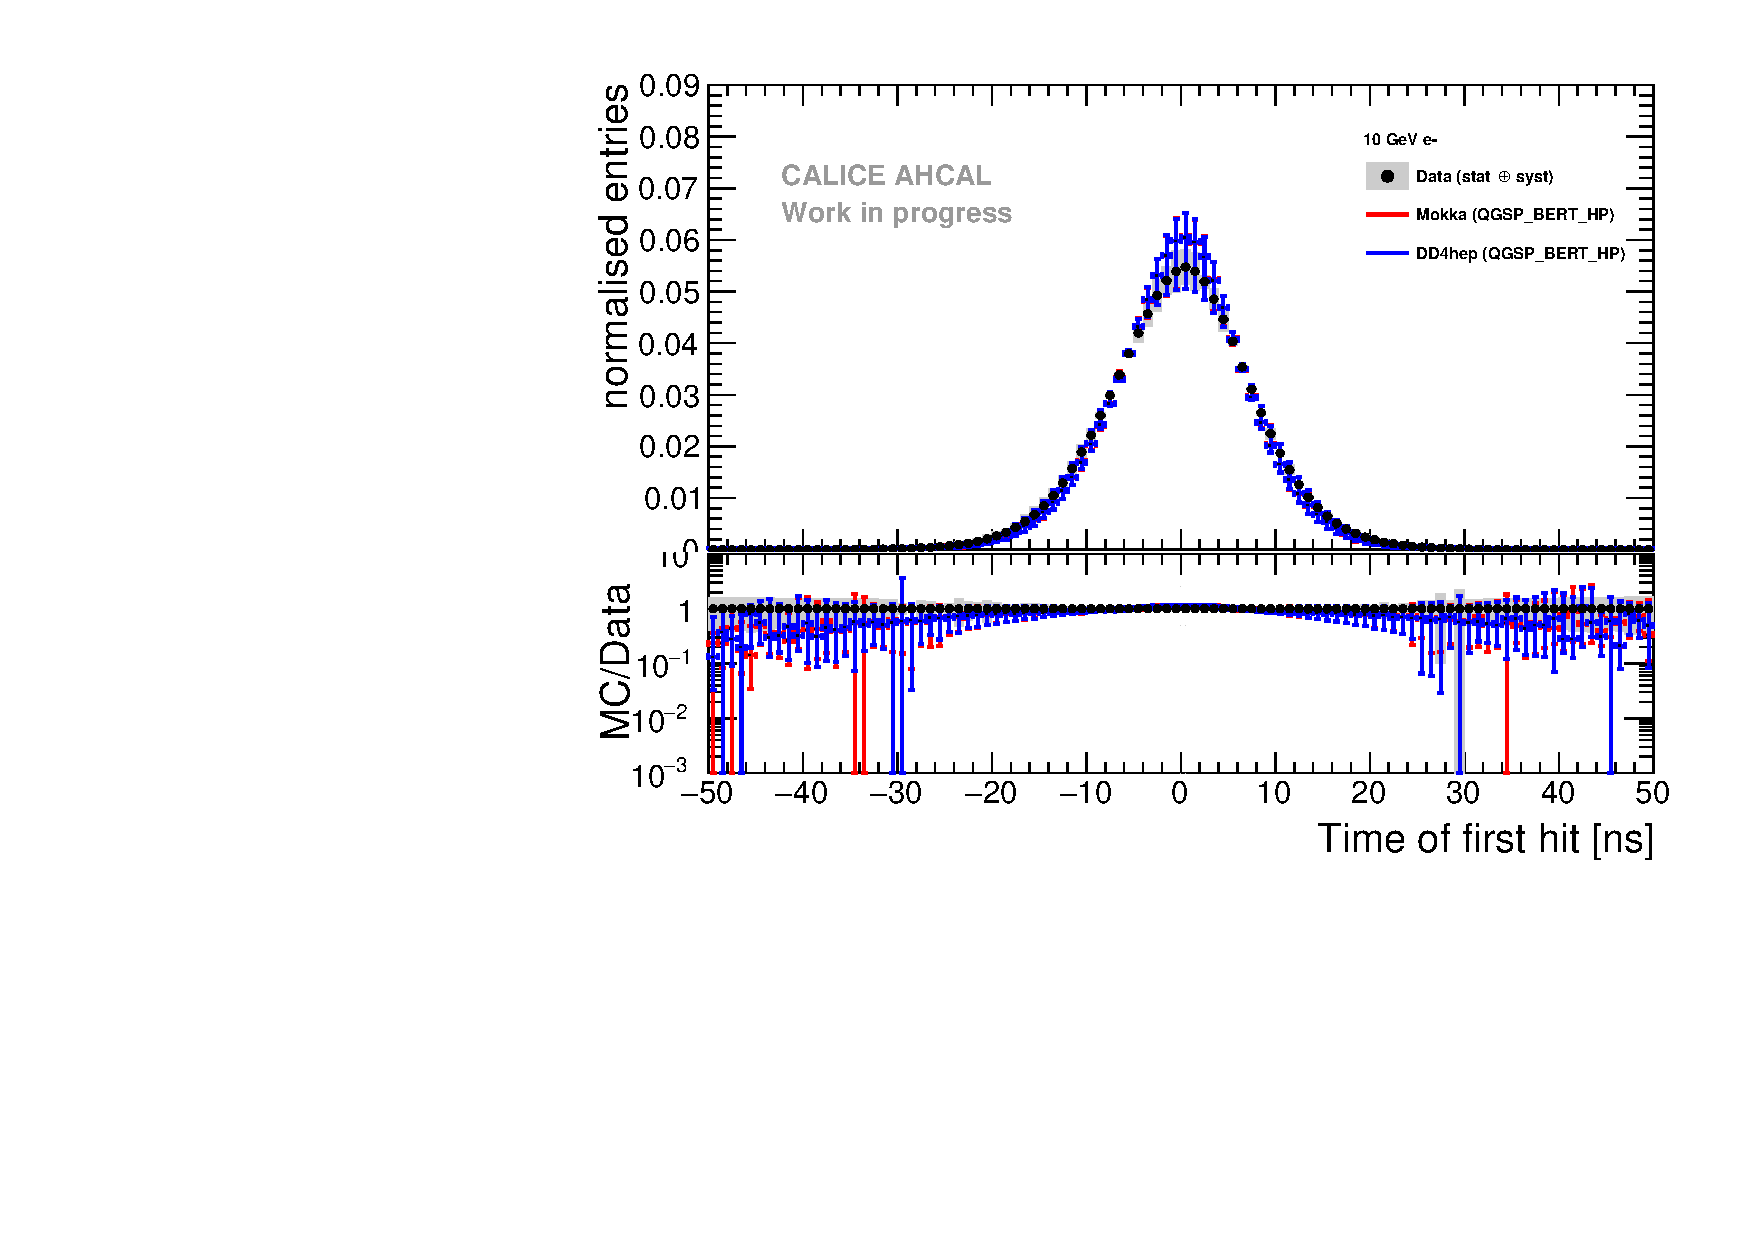
\includegraphics[width=1\textwidth]{fig/Comparison_SimData_Electrons10GeV.pdf}
		\caption{}\label{fig:elec_sim_data_10GeV}
	\end{subfigure}
	\hfill
	\begin{subfigure}[t]{0.49\textwidth}
		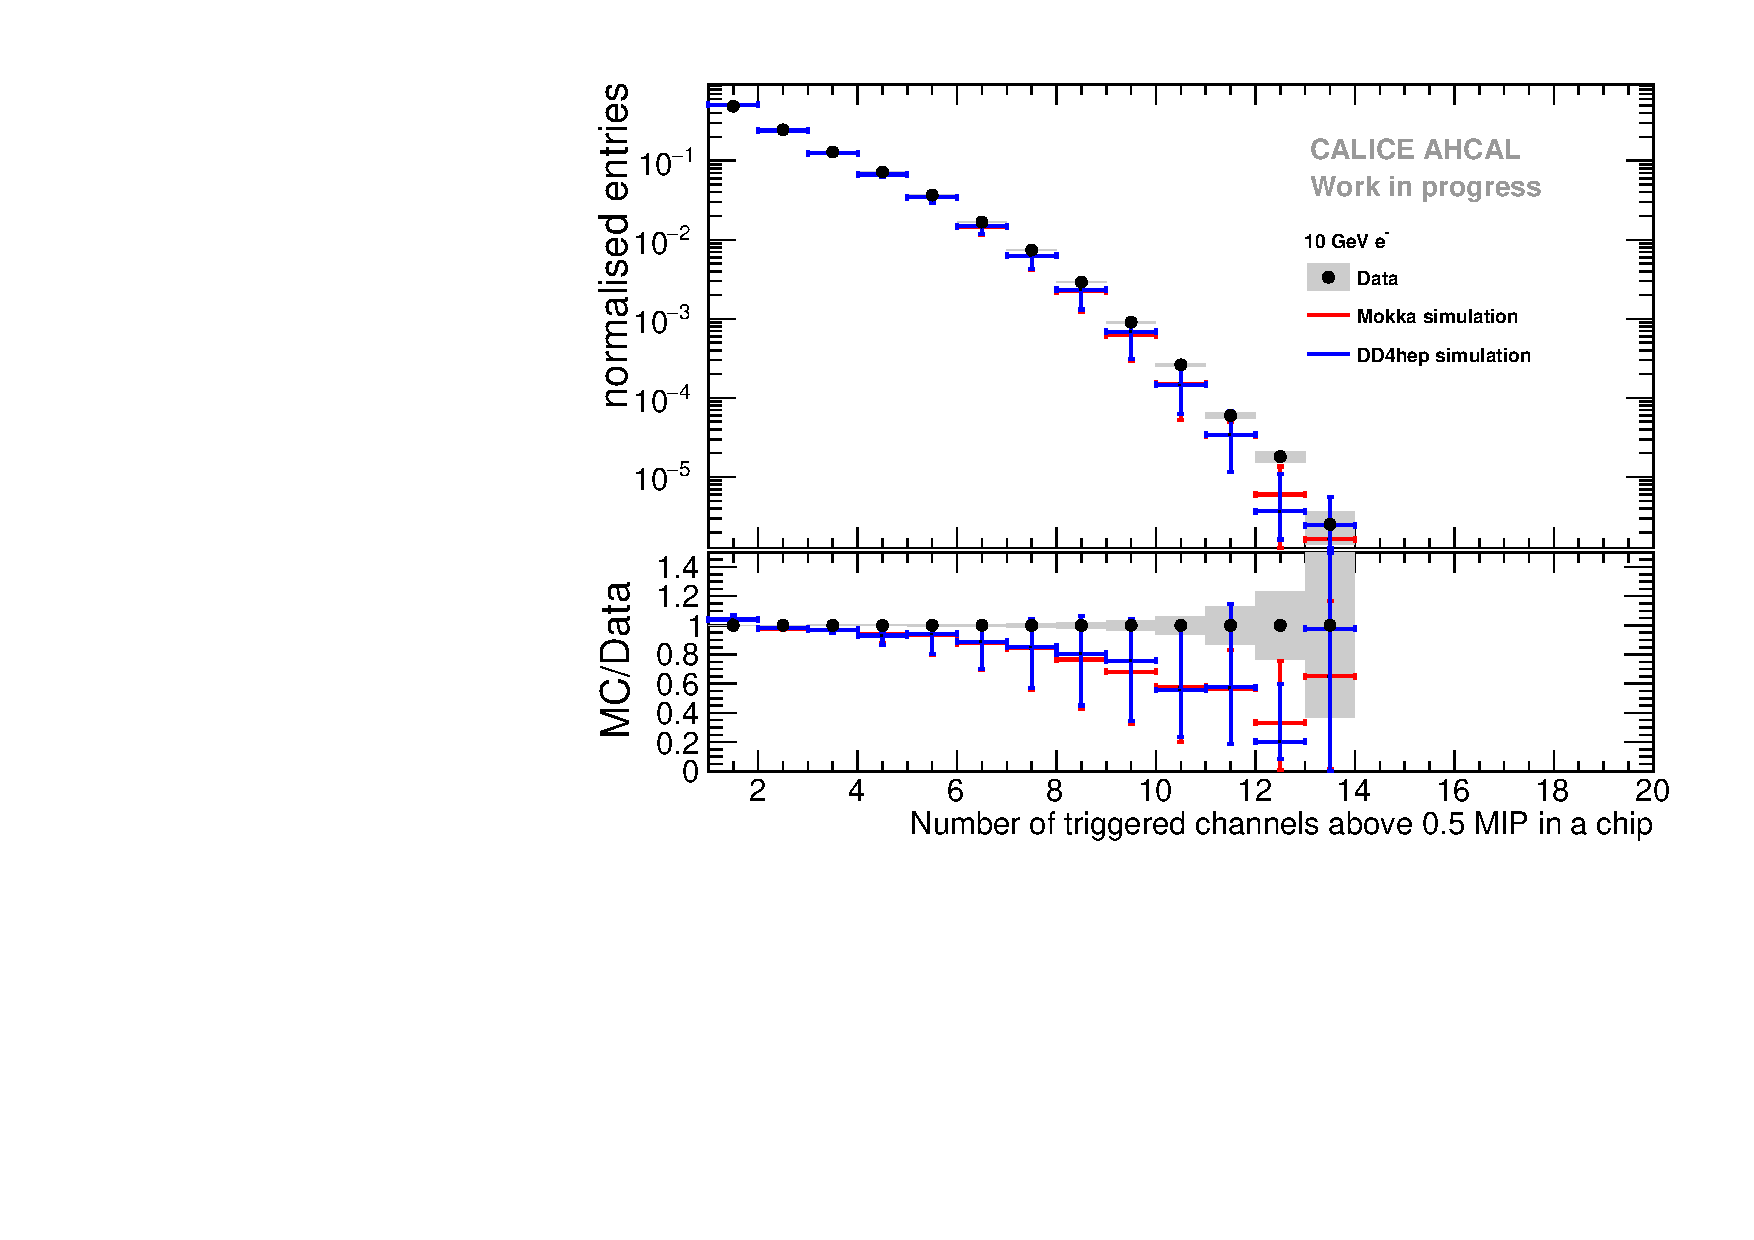
\includegraphics[width=1\textwidth]{fig/Comparison_SimData_Electrons_nHits_10GeV.pdf}
		\caption{}\label{fig:elec_sim_data_nHits_10GeV}
	\end{subfigure}
	\caption{\subref{fig:elec_sim_data_10GeV}) Comparison of the time of first hit between data and simulations for 10 GeV electrons. The grey area represents the statistical and systematical error of the data. Error bars in simulation are obtained by varying the cross-talk parameter between 10\% and 18\% and with the uncertainty on parametrization of the width of the time distribution as a function of the number of triggered channels in a chip. \subref{fig:elec_sim_data_nHits_10GeV}) Comparison of the number of triggered channels per chip between data and MC for 10 GeV electrons. The grey area represents the statistical error of the data. Error bars in simulation are obtained by varying the cross-talk parameter between 10\% and 18\%.}
\end{figure}

\subsection{Timing of pion showers}

The figure \ref{fig:dNdt_SimData_10GeV_all} shows the time distribution of first hits compared with three different physics lists for 10 GeV pions. For the core of the distribution under 50 ns, overall, all physics lists describe relatively well the data within the systematics. The QGSP\_BERT\_HP physics list reproduces well the distribution. The QBBC physics list tends to over-estimate the late tail by around a factor 2. This does not agree with the observations made in the T3B experiment \cite{Simon2013} where the QBBC physics list agrees well with the time distribution for 60 GeV pions. It may be related to the use of different \geant versions because the T3B experiment used \geant v9.4p03. The QGSP\_BERT physics list over-estimates the tail of the distribution by around a factor 10.

\begin{figure}[htbp!]
	\centering
	\begin{subfigure}[t]{0.49\textwidth}
		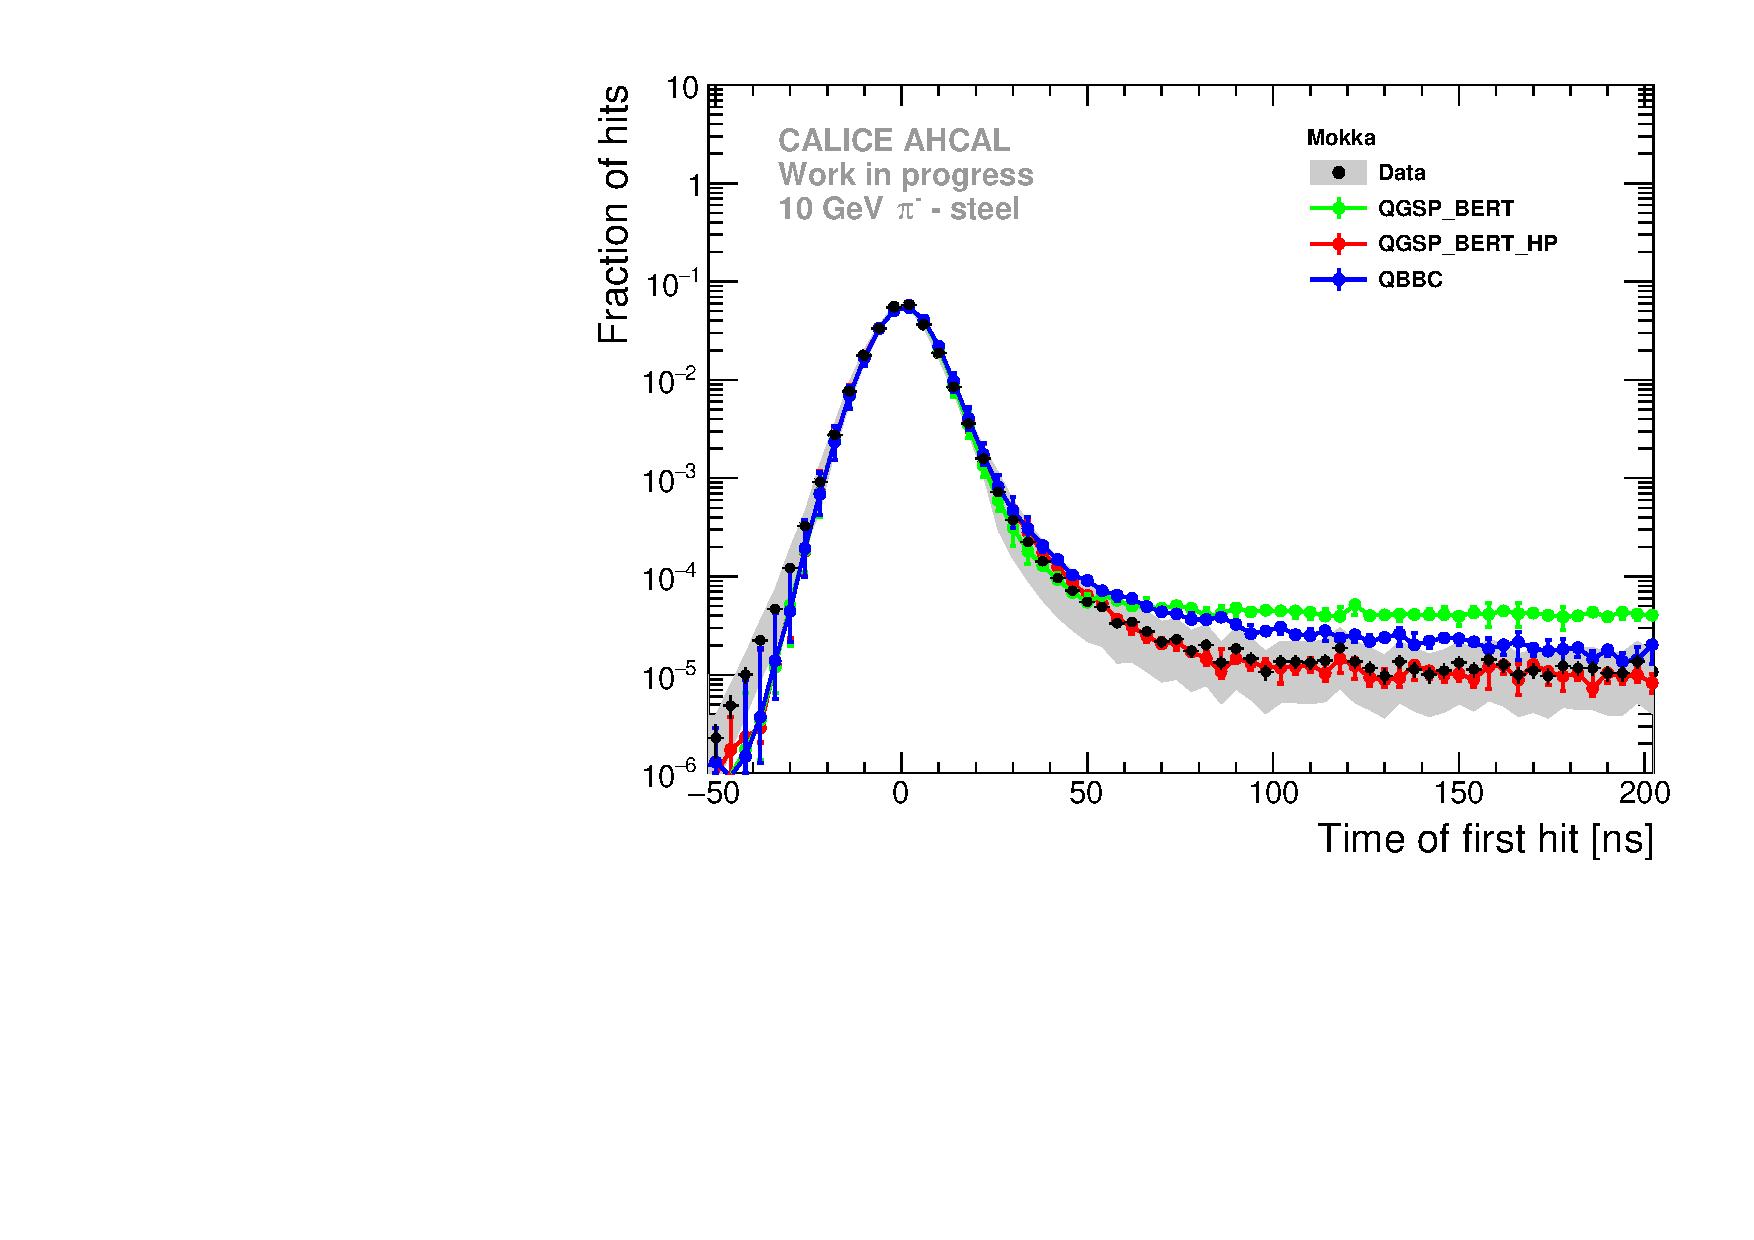
\includegraphics[width=1\textwidth]{fig/Comparison_SimData_Pion10GeV_LateClusters.pdf}
		\caption{}\label{fig:dNdt_SimData_10GeV}
	\end{subfigure}
	\hfill
	\begin{subfigure}[t]{0.49\textwidth}
		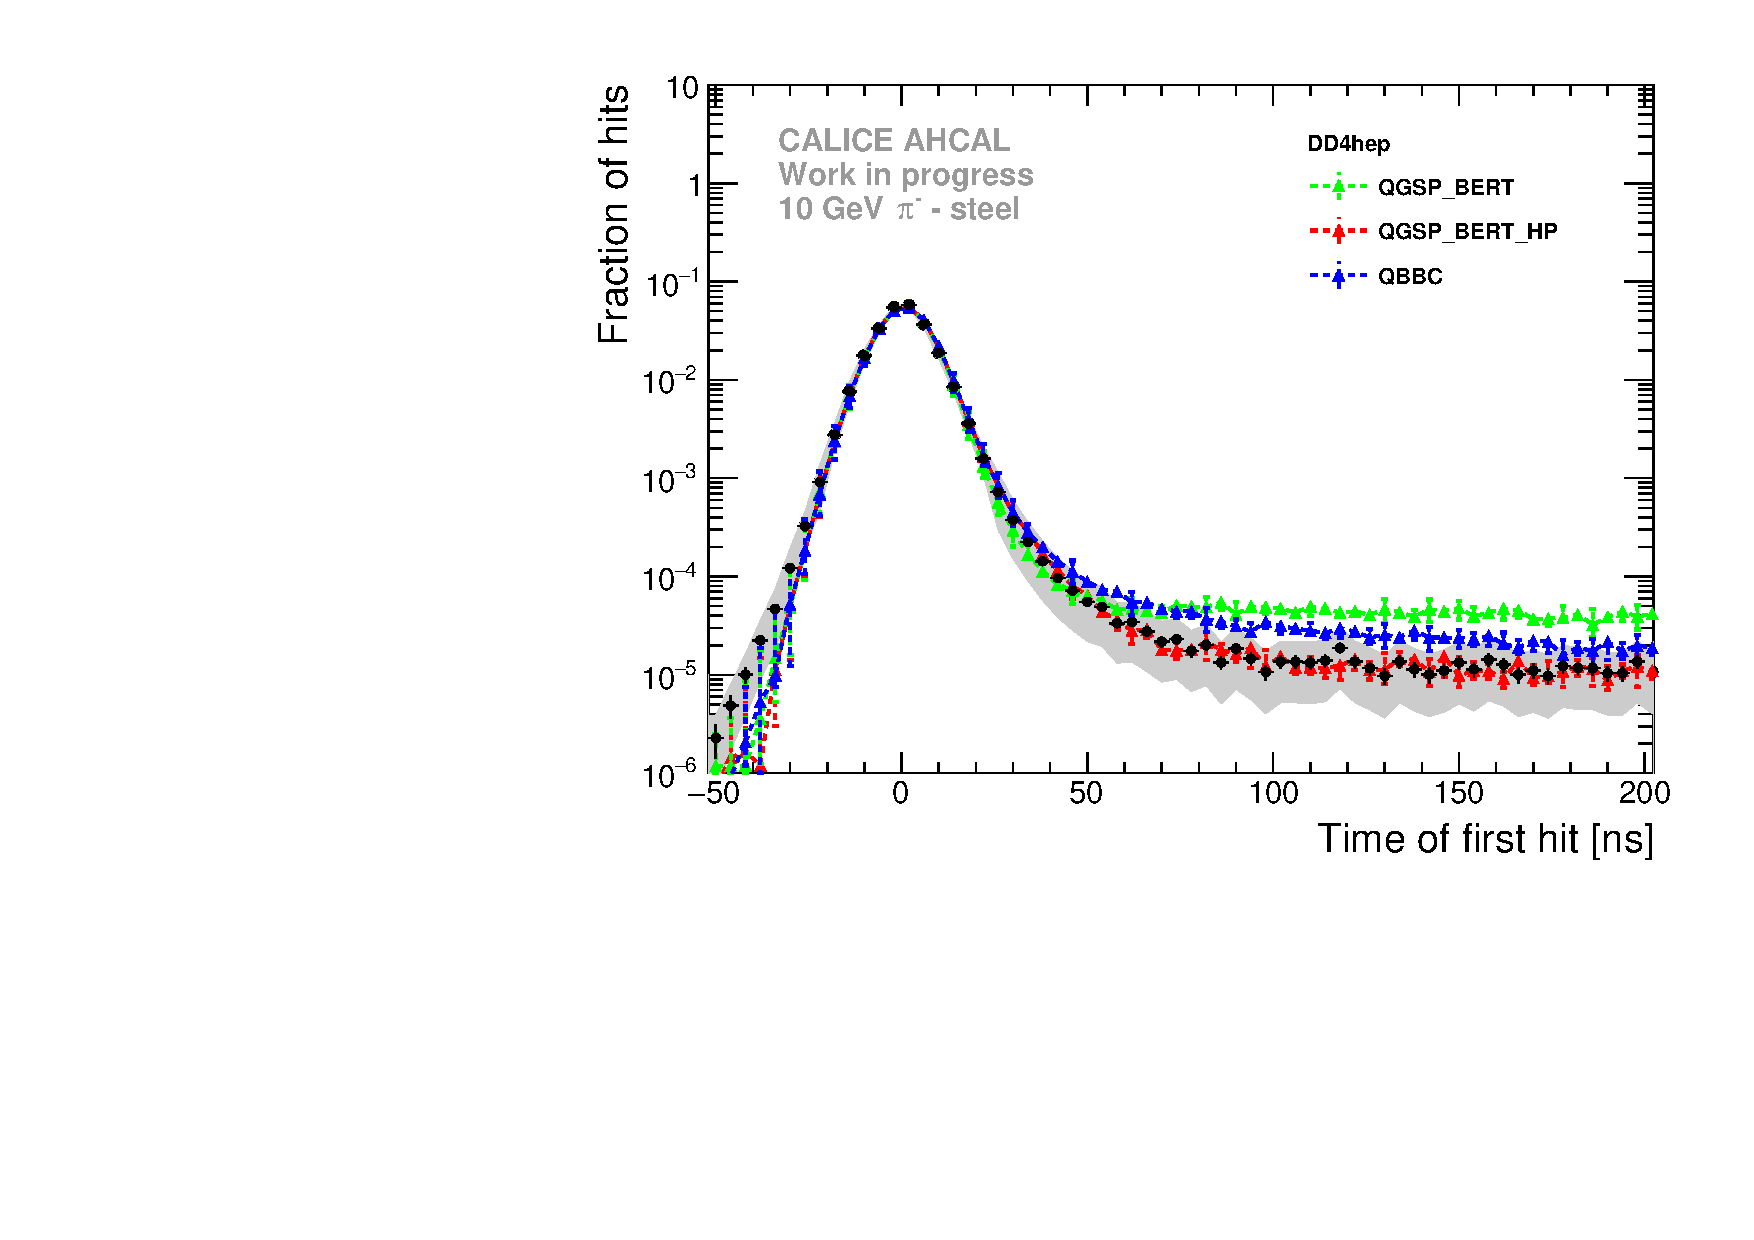
\includegraphics[width=1\textwidth]{fig/Comparison_SimData_Pion10GeV_LateClusters_DD4hep.pdf}
		\caption{}\label{fig:dNdt_SimData_10GeV_DD4hep}
	\end{subfigure}
	\caption{Comparison of the time of first hit distribution for 10 GeV pions in data and three different physics list for \mokka and \ddhep simulations. The grey and color bands shows the statistical and systematic uncertainties.}
	\label{fig:dNdt_SimData_10GeV_all}
\end{figure}

The dependence in energy of the time of first hit has been studied in the following. It is expected that there is no energy dependence for muon and electron beams as these are quasi-instantaneous. On the other hand, for pions, it is expected that low energy hits mostly coming from neutron signals in the calorimeter are delayed. The figures \ref{fig:Energy_SimData} show the comparison of the mean time of first hit as a function of the hit energy in data and simulations for 10 and 90 GeV pions. For 10 GeV pions, the simulation reproduces well the data within the systematics. However, for 90 GeV pions, a difference is visible in the region 0.5 to 1.5 MIP where the simulation is above the data. Above around 3 MIPs, the data and simulations agree well. Firstly, a difference is visible between the QGSP\_BERT and QGSP\_BERT\_HP physics lists mainly between hit energies of 1-3 MIPs but, in general, the difference is smaller than the systematic uncertainty on the data. Secondly, the QGSP\_BERT and QBBC physics lists are very similar over the full hit energy range. Finally, all models show an increase of the mean time of first hit at small hit energies with higher beam energy. The data does not reflect this. This comparison study seems to confirm that low energy hits are responsible for delayed energy depositions in the calorimeter, most likely due to low energy neutrons from capture and spallation processes. Higher energy deposits occur mostly in the prompt part of the hadron shower.

\begin{figure}[htbp!]
	\centering
	\begin{subfigure}[t]{0.49\textwidth}
		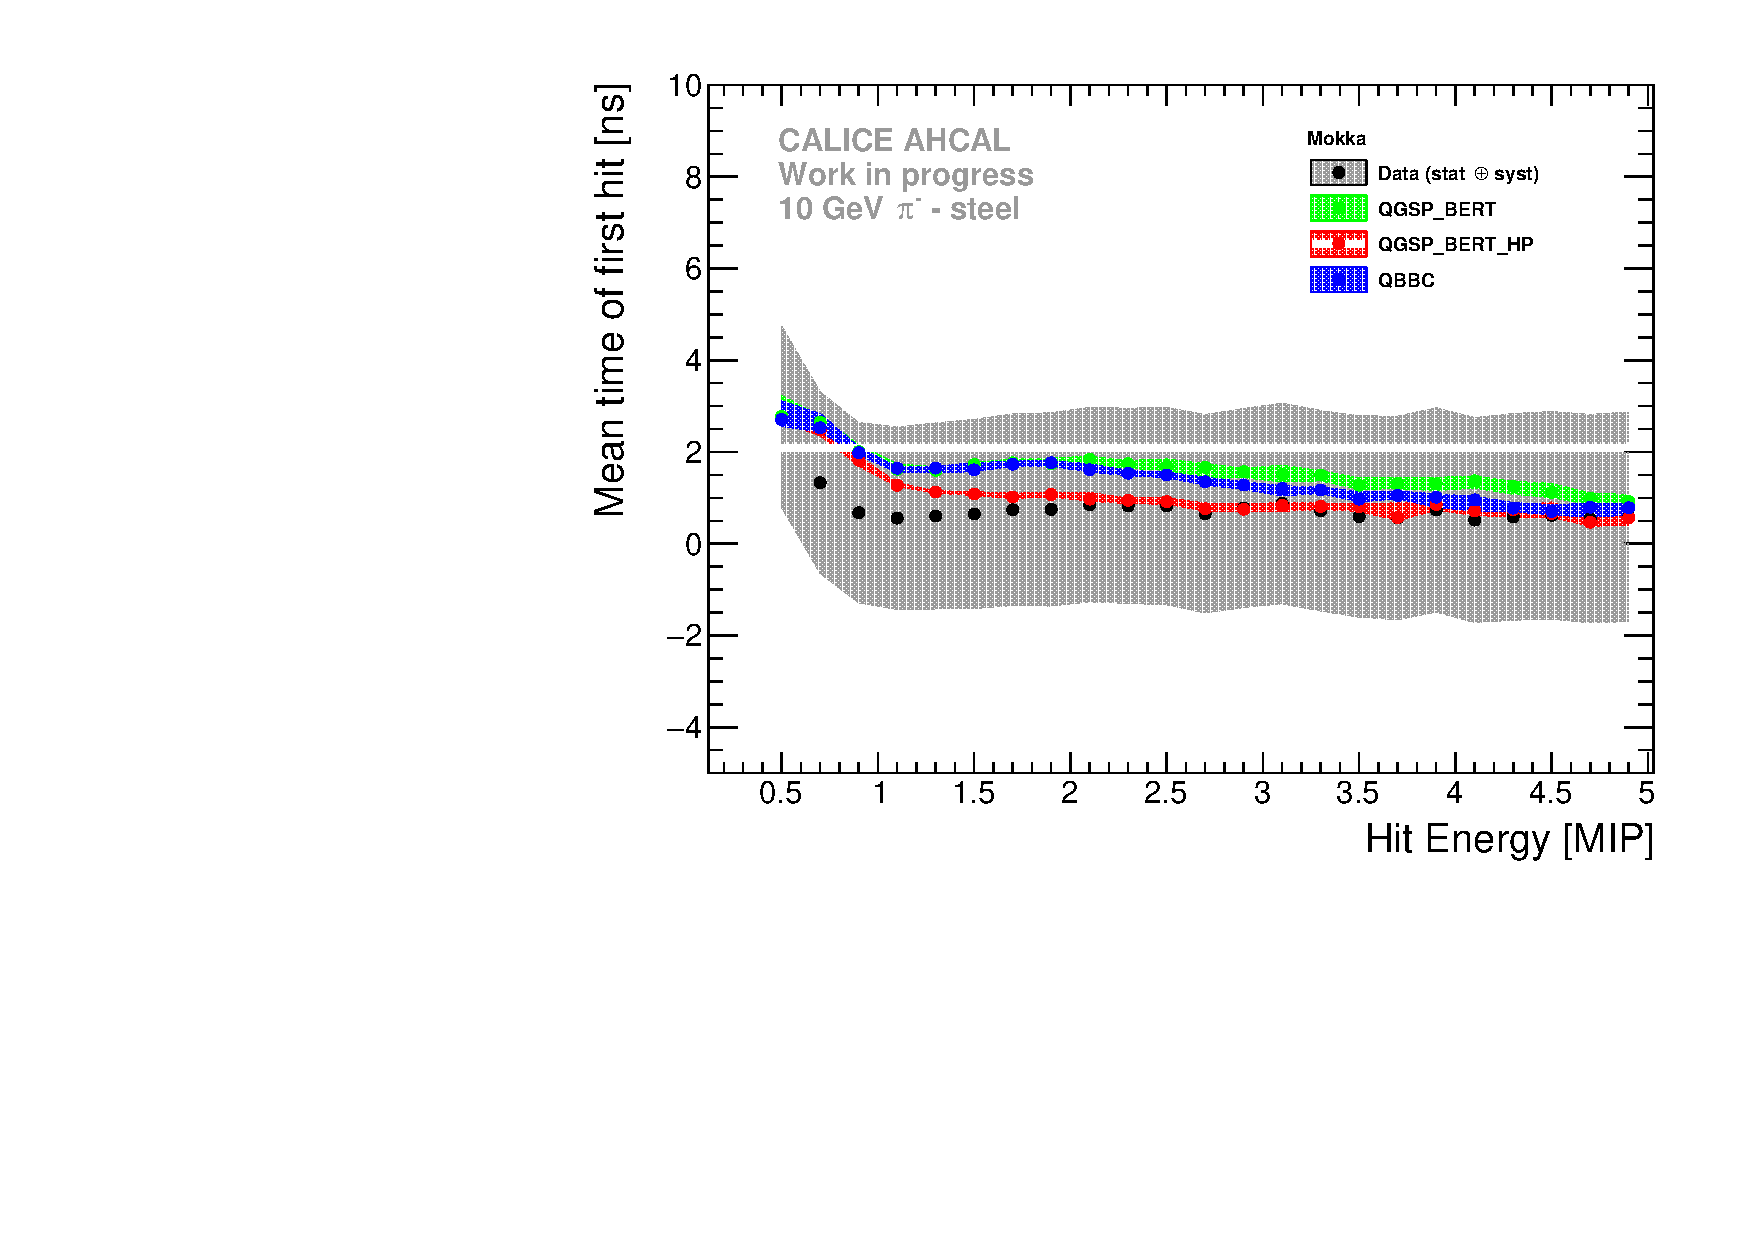
\includegraphics[width=1\textwidth]{fig/Time_Energy_10GeV_Mokka.pdf}
		\caption{}\label{fig:Energy_SimData_10GeV}
	\end{subfigure}
	\hfill
	\begin{subfigure}[t]{0.49\textwidth}
		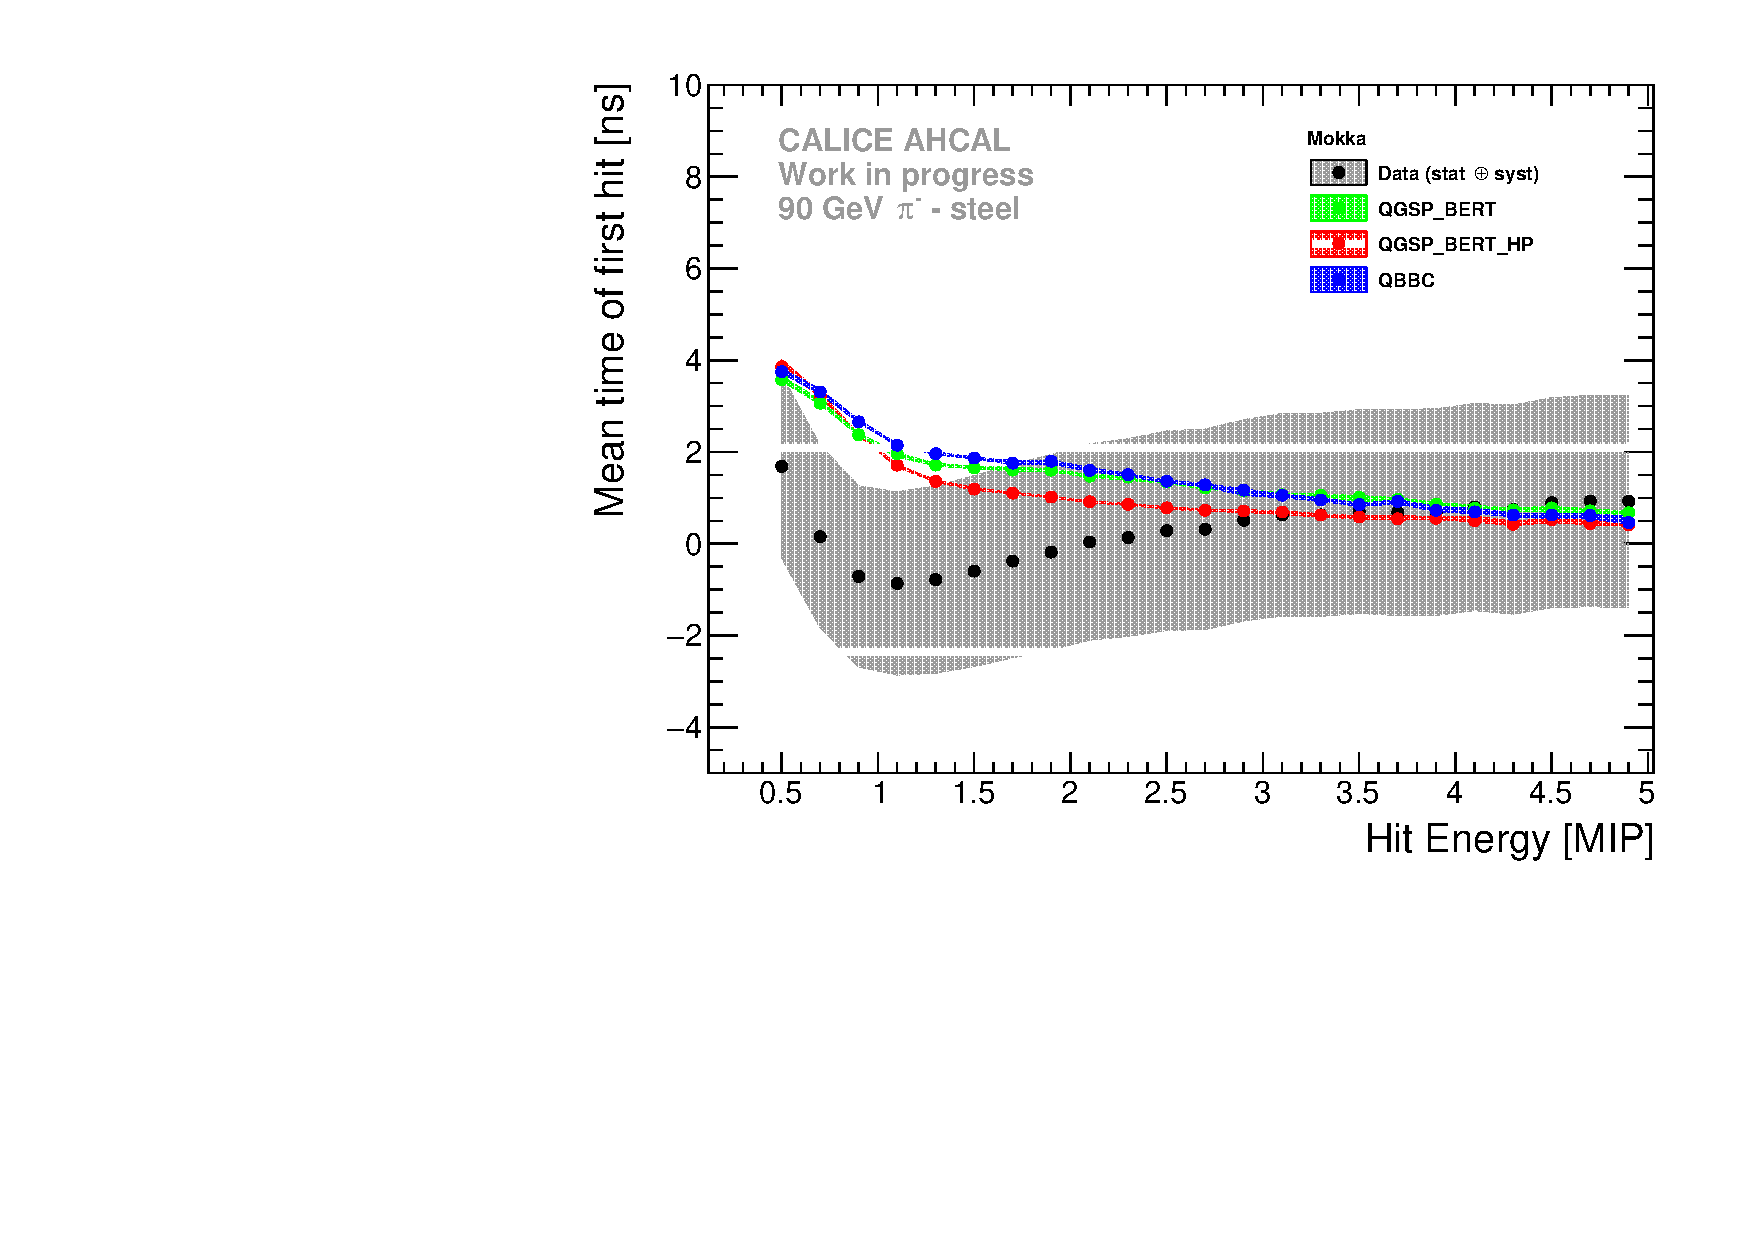
\includegraphics[width=1\textwidth]{fig/Time_Energy_90GeV_Mokka.pdf}
		\caption{}\label{fig:Energy_SimData_90GeV}
	\end{subfigure}
	\caption{Comparison of the mean time of first hit as function of the hit energy in data and simulations for 10 GeV and 90 GeV pions. The grey and color bands shows the statistical and systematic uncertainties.}
	\label{fig:Energy_SimData}
\end{figure}

The prompt component of a hadron shower is dominated by EM sub-showers and relativistic particles, whereas the delayed component is coming from mostly evaporation and spallation low energy neutrons. It is expected that the former is concentrated near the shower axis, while the latter, is spread out laterally as these neutrons can travel far away in the calorimeter before interacting. The radial dependence of the time of first hit of 50 GeV pion showers is compared to simulation as shown in figure \ref{fig:Radius_SSF_SimData_50GeVComparison}. For the layers 3 to 10, the QBBC and QGSP\_BERT\_HP physics lists reproduce well the data within systematics. The QGSP\_BERT physics list agrees well under a 10 cm distance and then starts to deviate from data up to 4-6 ns at 23 cm. Concerning the layers 11 to 14, over the full energy range, the QGSP\_BERT\_HP physics list agrees the best with the data. The QBBC and QGSP\_BERT physics lists agree with data up to around a 10 cm distance and then both lie above the data for higher distances, varing between few ns to 3-4 ns between 17 cm to 35 cm distance. The figures show that without neutron tracking in simulation, too many late energy depositions are created that are spread far away from the shower axis.

\begin{figure}[htbp!]
	\begin{subfigure}[t]{0.49\textwidth}
		\centering
		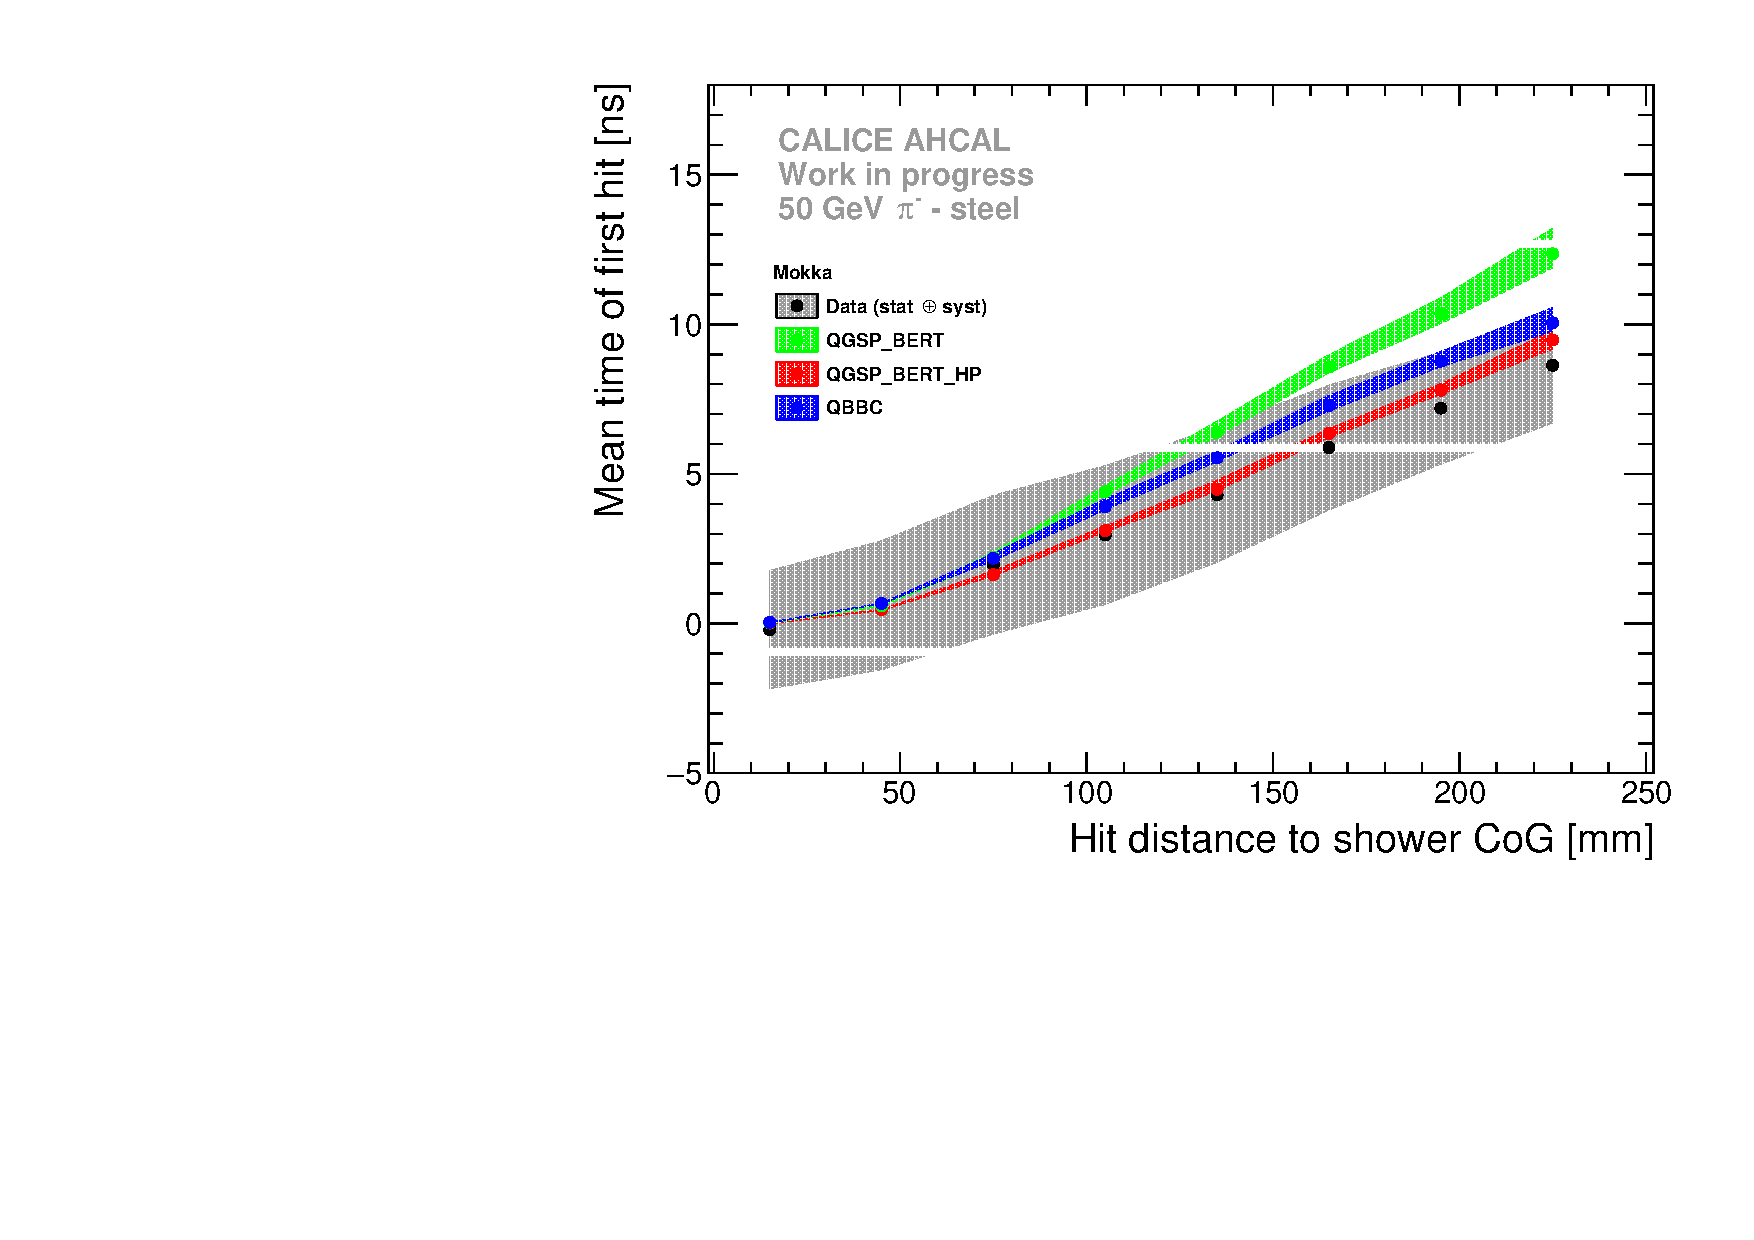
\includegraphics[width=1\textwidth]{fig/Time_Radius_50GeV_SSF_Mokka.pdf}
		\caption{Layers 3 to 10} \label{fig:Radius_SSF_SimData_50GeV}
	\end{subfigure}
	\hfill
	\begin{subfigure}[t]{0.49\textwidth}
		\centering
		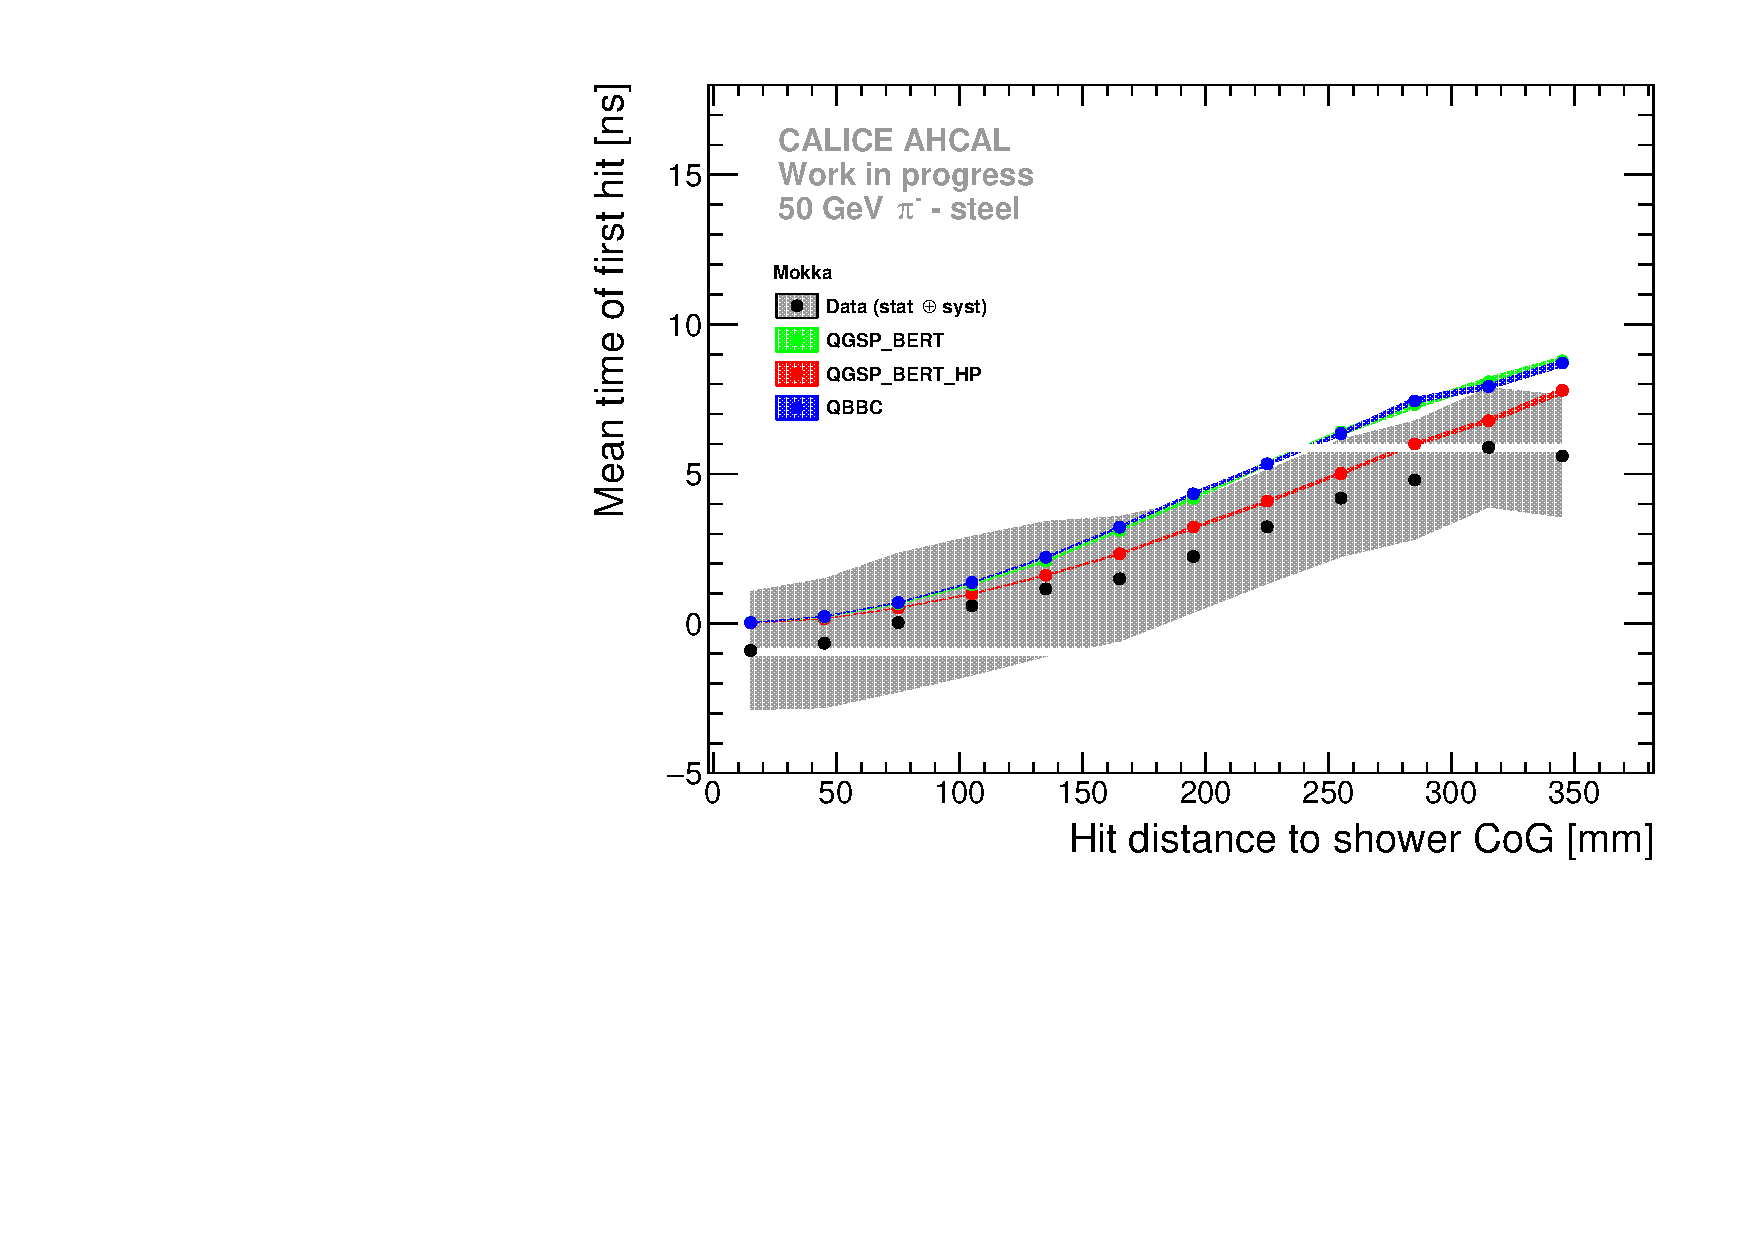
\includegraphics[width=1\textwidth]{fig/Time_Radius_50GeV_BL_Mokka.pdf}
		\caption{Layers 11 to 14} \label{fig:Radius_BL_SimData_50GeV}
	\end{subfigure}
	\caption{Comparison of the time of first hit as function of the hit distance to the shower axis in data and simulations for 50 GeV pion for the layers 3 to 10 on the left and for layers 11 to 14 on the right. The grey and color bands shows the systematics.}
	\label{fig:Radius_SSF_SimData_50GeVComparison}
\end{figure}

\section{Conclusion}

In this note, the timing study of the CALICE AHCAL technological prototype is presented, using the data taken at the CERN SPS in July 2015 in muon, electron and pion beams between 10 and 90 GeV.

Firstly, the timing calibration is presented. A time resolution of around 5 ns is achieved with muons and around 8 ns with electrons. The increase of the time resolution for electrons is due to an electronic effect that increase the time resolution depending on the number of hits within a chip.

Secondly, the time development of pion showers is presented. Late contributions are typically at low hit energies below 1 MIP and as well the late contributions are predominant at larger radius from the core of the shower. Comparisons to simulations show that the time structure of pion showers is well reproduced by the \geant physics lists QGSP\_BERT\_HP and QBBC. The QGSP\_BERT physics list tend to over-estimate the late contribution, showing that a proper treatment of neutrons is needed to reproduce the data to a satisfactory level.

% \acknowledgments

\bibliography{biblio}
\bibliographystyle{JHEP}
% \bibliographystyle{unsrt}

\clearpage

\appendix
\section{Appendix}

\begin{table}[htb!]
	\centering
	\caption{List of runs taken at SPS in July 2015.}
	\label{table:dataruns}
	\begin{tabular}{@{}lp{2cm}p{7.5cm}p{2cm}@{}}
		\toprule
		\multicolumn{1}{l}{\textbf{Particle}} & \textbf{Energy} & \textbf{Runs} & \textbf{\# Events}\\
		\midrule
		\multirow{2}{*}{$\mu^-$}& 50 GeV & 24016-24204 & 120,887,651\\& 150 GeV & 24623-24662 & 15,534,328\\
		\midrule
		\multirow{2}{*}{e$^-$}& 10 GeV & 24531-24576 & 38,028,438\\& 15 GeV & 24507-24527 & 7,701,325\\& 20 GeV & 24479-24504 & 10,498,554\\& 30 GeV & 24454-24475 & 3,382,943\\& 40 GeV & 24420-24448 & 2,665,843\\& 50 GeV & 24404-24419 & 5,933,995\\
		\midrule
		\multirow{2}{*}{$\pi^-$}& 10 GeV & 24266-24272, 24300-24317, 24381-24397 & 24,311,420\\& 20 GeV & 24398-24400 & N/A\\& 30 GeV & 24259-24299, 24319-24380 & 10,120,753\\& 50 GeV & 24212-24254, 24325-24357, 24580-24612 & 10,704,661\\& 70 GeV & 24219-24242, 24365-24374 & 8,885,407\\& 90 GeV & 24233-24287, 24331-24364 & 7,955,604\\
		\bottomrule
	\end{tabular}
\end{table}

\begin{table}[htb!]
	\centering
	\caption{List of AHCAL channels used as time reference for this analysis. In this analysis, the time reference signals T$_{12}$, T$_{13}$ and T$_{14}$ are used.}
	\label{table:trigger_ref}
	\begin{tabular}{@{} ccccc @{}}
		\toprule
		Layer \# & Chip Number & Channel & Comments & Name \\
		\midrule
		11 & 169 & 29 & noisy & T$_{11}$ \\
		11 & 177 & 23 & broken & - \\
		12 & 185 & 29 & - & T$_{12}$ \\
		13 & 201 & 29 & -  & T$_{13}$ \\
		13 & 211 & 6 & broken & - \\
		14 & 217 & 23 & - & T$_{14}$ \\
		\bottomrule
	\end{tabular}
\end{table}

\begin{table}[htb!]
	\centering
	\caption{Selection cuts for the muon runs.}
	\label{table:muon_sel}
	\begin{tabular}{@{}lll@{}}
		\toprule
		\multicolumn{1}{l}{\textbf{Name}} & \textbf{Beam Energy} & \textbf{Cut}\\
		\midrule
		\multirow{2}{*}{Preselection}& All & 0 mm < $cog_{z}$ < 800 mm\\& All & 0 < $n_{hits}$ < 20 \\
		\multirow{2}{*}{Track Selection SSF}& All & $n_{hits}$ in tower > 7 \\& All & $n_{hits}$ in layer < 3 \\
		\multirow{2}{*}{Track Selection BL}& All & $n_{hits}$ in tower > 2 \\& All & $n_{hits}$ in layer < 3 \\
		\bottomrule
	\end{tabular}
\end{table}

\begin{table}[htb!]
	\centering
	\caption{Selection cuts for each electron runs.}
	\label{table:electron_sel}
	\begin{tabular}{@{}lll@{}}
		\toprule
		\multicolumn{1}{l}{\textbf{Name}} & \textbf{Beam Energy} & \textbf{Cut}\\
		\midrule
		\multirow{2}{*}{Event Quality}& All & Cherenkov ON\\& All & Energy in the first 3 layers of AHCAL > 10 MIP \\
		\multirow{9}{*}{Electron Selection}& 10 GeV & 25 < $n_{hits}$ < 75 \\& 15 GeV & 30 < $n_{hits}$ < 90 \\& 20 GeV & 40 < $n_{hits}$ < 100 \\& 30 GeV & 50 < $n_{hits}$ < 110 \\& 40 GeV & 60 < $n_{hits}$ < 120 \\& 50 GeV & 70 < $n_{hits}$ < 140 \\& All & $cog_{z}$ < 250 mm\\& All & -90 mm < $cog_{x, y}$ < 90 mm \\& All & Energy in last two layers < 1\% $E_{sum}$ \\
		\bottomrule
	\end{tabular}
\end{table}

\begin{table}[htb!]
	\centering
	\caption{Selection cuts for the pions runs.}
	\label{table:pion_sel}
	\begin{tabular}{@{}lll@{}}
		\toprule
		\multicolumn{1}{l}{\textbf{Name}} & \textbf{Beam Energy} & \textbf{Cut}\\
		\midrule
		\multirow{1}{*}{Event Quality}& All & Cherenkov OFF\\
		\multirow{3}{*}{Pion Selection}& All & $n_{hits}$ > 20 \\& All & $n_{hits}$ in the first 2 AHCAL layers < 5 \\& All & Energy in last two layers > 1\% $E_{sum}$ \\
		\multirow{2}{*}{Multi Particle Rejection}& All & $n_{hits}$ in time window > 5 \\& All & $n_{Cluster}$ > 0 \\
		\bottomrule
	\end{tabular}
\end{table}

\begin{table}[htb!]
  \centering
  \caption{List of the different SiPMs used in the CALICE AHCAL in July 2015.}
  \label{table:sipm_list}
  \resizebox{\textwidth}{!}{%
  \begin{tabular}{@{}cccccccc@{}}
    \toprule
    Layer & Producer & Model & Area (mm$^2$) & Pitch ($\mu$m) & WLS Fibre & Read-out type & $N_{px}$ [$10^3$]\\
    \midrule
    1 & Hamamatsu & S12571\_010P & $1\times1$ & 10 & no & Bottom & 10\\
    2 & Hamamatsu & S10362-11-025O & $1\times1$ & 25 & no & Side & 1.6\\
    3 & Hamamatsu & S12571-025P & $1\times1$ & 25 & no & SMD & 1.6\\
    4-5 & Ketek & N/A & $2.25\times2.25$ & 18 & no & Side & 12\\
    6-10 & CPTA & CPTA & $1.28\times1.28$ & 40 & yes & Side & 0.8\\
    11-12 & Ketek (UHH) & PM1125NS-SB0 & $1.2\times1.2$ & 25 & no & Side & 2.3\\
    13-14 & SenSL & MicroFB-10020-SMT & $1\times1$ & 20 & no & Side & 1.3\\
    \bottomrule
  \end{tabular}
  }
\end{table}

\end{document}
